%%
%% abtex2-modelo-trabalho-academico.tex, v-1.9.2 laurocesar
%% Copyright 2012-2017 by abnTeX2 group at http://abntex2.googlecode.com/ 
%%
%% This work may be distributed and/or modified under the
%% conditions of the LaTeX Project Public License, either version 1.3
%% of this license or (at your option) any later version.
%% The latest version of this license is in
%%   http://www.latex-project.org/lppl.txt
%% and version 1.3 or later is part of all distributions of LaTeX
%% version 2005/12/01 or later.
%%
%% This work has the LPPL maintenance status `maintained'.
%% 
%% The Current Maintainer of this work is Emílio Eiji Kavamura,
%% eek.edu@outlook.com; emilio.kavamura@ufpr.br
%% Further information about abnTeX2 are available on 
%%
%% http://abntex2.googlecode.com/
%%
%% https://code.google.com/p/abntex2/issues/ 
%%
%% Further information about UFPR abnTeX2 are available on 
%%
%% https://github.com/eekBR/ufpr-abntex/
%%
%% This work consists of the files 
% 
%              main.tex   programa principal
%          00-dados.tex   entrada de dados 
%          00-pacotes.tex   pacotes carregados no modelo
% 00-pacotesOpcionais.tex   pacotes opcionais
      % 00-pretextual.tex   processamento dos elementos pre-textuais
%                UFPR.sty   ajusta do modelo canonico às normas  UFPR
%
%    referencias.bib
%                     e outras arquivos de imagens
%
%
%------------------------------------------------------------------------
% ------------------------------------------------------------------------
% abnTeX2: Modelo de Trabalho Academico (tese de doutorado, dissertacao de
% mestrado e trabalhos monograficos em geral) em conformidade com 
% ABNT NBR 6023:2018: Informação e documentação - Referências - Elaboração
% ------------------------------------------------------------------------
% ------------------------------------------------------------------------
%
% DATA DE ATUALIZAÇÃO: 2025-05-27

\documentclass[
        % -- opções da classe memoir --
        12pt,                           % tamanho da fonte
        openright,                      % capítulos começam em pág ímpar (insere página vazia caso preciso)
        %twoside,                        % para impressão em verso e anverso. Oposto a oneside
        oneside,
        a4paper,                        % tamanho do papel. 
        % -- opções da classe abntex2 --
        chapter=TITLE,         % títulos de capítulos convertidos em letras maiúsculas
        section=TITLE,         % títulos de seções convertidos em letras maiúsculas
        subsection=Title,      % títulos de subseções convertidos em letras maiúsculas
        %subsubsection=TITLE,  % títulos de subsubseções convertidos em letras maiúsculas
        % -- opções do pacote babel --
        english,                        % idioma adicional para hifenização
        %french,                         % idioma adicional para hifenização
        spanish,                        % idioma adicional para hifenização
        portugues,                      % o último idioma é o principal do documento
        %%%%%%%%%%%%
        %eek: colocação da opção para o sumario ter formatação tradicional
        %sumario=tradicional             % título no formato tradicional
        ]{abntex2}

\usepackage{UFPR}
% Pacotes básicos 
% ----------------------------------------------------------
%\usepackage{lmodern}			% Usa a fonte Latin Modern			
\usepackage[T1]{fontenc}		% Selecao de codigos de fonte.
\usepackage[utf8]{inputenc}		% Codificacao do documento (conversão automática dos acentos)
\usepackage{lastpage}			% Usado pela Ficha catalográfica
\usepackage{indentfirst}		% Indenta o primeiro parágrafo de cada seção.
\usepackage{microtype} 			% para melhorias de justificação
\usepackage{ifthen}		    	% para montar condicionais
\usepackage[brazil]{babel}		% para utilizar termos em portugues
\usepackage[final]{pdfpages}    % para incluir páginas de arquivos pdf
\usepackage{amsmath}			% simbolos matematicos

% Pacotes de citações BibLaTeX
% ----------------------------------------------------------
\usepackage[style=abnt,
	backref=true,
	backend=biber,
	citecounter=true,
	backrefstyle=three, 
 	repeatfields=true,
	url=true,
	maxbibnames=99,
    mincitenames=1,
    maxcitenames=2,
    backref=true,
    hyperref=true,
    giveninits=true,
    uniquename=false,
    uniquelist=false]{biblatex}

% Norma NBR10.520/2023 - Sobrenomes em minúsculas
\renewcommand*{\mkbibnamefamily}[1]{#1}%

% Espaçamento entre os itens nas referências (espço de uma linha simples)
% ----------------------------------------------------------
\setlength\bibitemsep{\baselineskip}

% Texto padrão para as referências
% ----------------------------------------------------------
\DefineBibliographyStrings{brazil}{%
	 backrefpage  = {Citado \arabic{citecounter} vez na página},		% originally "cited on page"
	 backrefpages = {Citado \arabic{citecounter} vezes nas páginas},	% originally "cited on pages"
	 urlfrom      = {Dispon\'ivel em},
}

% Ajusta indentação de Referencias no ToC
% ----------------------------------------------------------
\defbibheading{bay}[\bibname]{%
  \chapter*{#1}%
  \markboth{#1}{#1}%
  \addcontentsline{toc}{chapter}
  %{\protect\numberline{}\bibname}
  {\bibname}
}

% Formatando o avançao dos títulos no sumário 
% ----------------------------------------------------------
\makeatletter
	\pretocmd{\chapter}{\addtocontents{toc}{\protect\addvspace{-12\p@}}}{}{}
	\pretocmd{\section}{\addtocontents{toc}{\protect\addvspace{-3\p@}}}{}{}
\makeatother

% https://groups.google.com/g/abntex2/c/ZYwE4t9uTFM
\makeatletter
\let\oldcontentsline\contentsline
\def\contentsline#1#2{%
	\expandafter\ifx\csname l@#1\endcsname\l@section
	\expandafter\@firstoftwo
	\else
	\expandafter\@secondoftwo
	\fi
	{%
		\oldcontentsline{#1}{\MakeTextUppercase{#2}}%
	}{%
		\oldcontentsline{#1}{#2}%
	}%
}
\makeatother

% Para retirar os símbolos <> da URL  
% ----------------------------------------------------------
\DeclareFieldFormat{illustrated}{\addspace #1\isdot}%
%\DeclareFieldFormat{url}{\bibstring{urlform}\addcolon\addspace<\url{#1}>}%
%\DeclareFieldFormat{url}{\bibstring{urlfrom}\addcolon\addspace<\url{#1}>}%
\DeclareFieldFormat{url}{\bibstring{urlfrom}\addcolon \space\addspace{#1}} 
% remove <> em urls de acordo com abnt-6023:2018	

% Ajustar o espaço para a formatação da data
% ----------------------------------------------------------
\DeclareFieldFormat{urldate}{\bibstring{urlseen}\addcolon\addspace #1}%
\DeclareFieldFormat*{note}{\addspace #1}%

% Para ajustar o tamanho da fonte do número da primeira página do capítulo
% comando utilizado na parte textual 
% ----------------------------------------------------------
\makepagestyle{chapfirst}% Just for the first page of a chapter
\makeoddhead{chapfirst}{}{}{\footnotesize{\thepage}}

%%criar um novo estilo de cabeçalhos e rodapés
\makepagestyle{simplestextual}
  %%cabeçalhos
  \makeevenhead{simplestextual} %%pagina par
     {}{}{\footnotesize \thepage}
     
  \makeoddhead{simplestextual} %%pagina ímpar ou com oneside
     {}{}{\footnotesize \thepage}
  %\makeheadrule{simplestextual}{\textwidth}{\normalrulethickness} %linha
  %% rodapé
  \makeevenfoot{simplestextual}
     {}{}{} %%pagina par
      
  \makeoddfoot{simplestextual} %%pagina ímpar ou com oneside
     {}{}{}
     
% Define a formatação dos capítulos póstextuais numerados
% ----------------------------------------------------------
%\newcommand{\refap}[1]{\hyperref[#1]{Apêndice~\ref{#1}}} 	% Referência apÊndices



 %%%%%%%%%%% NBR 10520/23

 % Norma NBR10.520/2023 - Sobrenomes em minúsculas
\renewcommand*{\mkbibnamefamily}[1]{#1}%

%fullcite com todos autores e não como cite
\makeatletter
\newcommand{\tempmaxup}[1]{\def\blx@maxcitenames{99}#1}
\makeatother

\DeclareCiteCommand{\fullcite}[\tempmaxup]
{\usebibmacro{prenote}}
{\usedriver
	{}
	{\thefield{entrytype}}}
{\multicitedelim}
{\usebibmacro{postnote}}

\usepackage{graphicx}
\usepackage{enumitem}
\usepackage{float}
\usepackage{changepage}

\usepackage{tabularx}

\usepackage{color}		    	% Controle das cores
\usepackage{graphicx}			% Inclusão de gráficos
\usepackage{lipsum}				% para geração de dummy text
\usepackage{csquotes}

%\usepackage[style=long]{glossaries}
%\usepackage{abntex2glossaries}

\usepackage{cancel} 		% permite representar o cancelamento de termos em texto ou equacoes	
\usepackage{xcolor} 		% cores extendidas	
\usepackage{smartdiagram}   	% gera diagramas a partir de listas
%\usepackage{float} 		% Para a figura ficar na posição correta	    
\usepackage{textcomp} 		% supporte para fontes da Text Companion 
\usepackage{longtable}		% uso de longtable

\usepackage{lscape}		% páginas em paisagem
\usepackage{multicol}		% mescla de colunas em tabelas
\usepackage{multirow}		% mescla de linhas em tabelas
\usepackage{newfloat} 		% criação do indice de quadros
%\usepackage{caption} 		% configura legenda 
%[format=plain]
%\renewcommand\caption[1]{%
	%\captionsetup{font=small}	% tamanho da fonte 10pt
	%,format=hang
	% \caption{#1}}
%\captionsetup{width=0.8\textwidth}
\captiondelim{-- }
\captiontitlefont{\small}
\captionnamefont{\small}


% uso do tikz e pgfplots
% ----------------------------------------------------------
%\usetikzlibrary{external}
\usetikzlibrary{arrows,calc,patterns,angles,quotes}
\usepackage{pgfplots}
\pgfplotsset{compat=1.15}


% Define o comando para citação de fontes em elementos gráficos (figuras, imagens,...).
% ----------------------------------------------------------
%  AUTOR(ano)
%
% parâmetro é a bibkey da fonte

\newcommand{\citefig}[2]{~\Citeauthor*{#1}\citeyear{#1}}

% Define os operadores matemáticos em portugues
% ----------------------------------------------------------
%

\DeclareMathOperator{\tr}{tr}
\DeclareMathOperator{\sen}{sen}
\DeclareMathOperator{\senh}{senh}
%\DeclareMathOperator{\tag}{tag}
\DeclareMathOperator{\tg}{tg}
\DeclareMathOperator{\tagh}{tagh}
\DeclareMathOperator{\tgh}{tgh}
\DeclareMathOperator{\cossec}{cossec}
%\DeclareMathOperator{\sen}{sen}

% Para fazer a listagem de codigos LaTeX na documentação
% ----------------------------------------------------------
\usepackage{listings}

% Comando para fazer 
%    a citação de documentos não publicados e informais e 
%    colocar as referências nas notas de rodapé
% ----------------------------------------------------------

\newcommand{\citenp}[1]{
	\cite{#1}\footnote{\fullcite{#1}}}

\newcommand{\textcitenp}[1]{
	\textcite{#1}\footnote{\fullcite{#1}}}


% para comentarios e sugestões
% ----------------------------------------------------------
\newcommand{\sugest}[1]{\textcolor{red!40}{#1}}


% simplificação para colocar figuras
% ----------------------------------------------------------
%   Parametros
%    1 caption
%    2 percent textwidth
%    3 arquivo da figura
%    4 fonte
%    5 fig:label
%    6 nota
%    7 legenda

\newcommand{\figura}[7]{
  {\centering
   \footnotesize
   \begin{figure}[!ht]
   \centering
        \caption{\uppercase{#1}}
        \includegraphics[width=#2\textwidth]{#3}
        \label{fig:#5}
    
    %ajustado p/ a largura da imagem
    \begin{minipage}{#2\textwidth} 
        \vspace{2mm}\centering
        %\begin{flushleft}
            \par FONTE:~#4
            \ifthenelse{\equal{#6}{}}{}
            { \par\hangindent=14mm NOTA: #6 }
            
            \ifthenelse{\equal{#7}{}}{}
            { \par\hangindent=14mm LEGENDA: #7 }
        %\end{flushleft}
    \end{minipage}
    \end{figure}
    }
}


% simplificação para colocar figuras cortadas
% ----------------------------------------------------------
%   Parametros
%    1 caption
%    2 percent textwidth
%    3 arquivo da figura
%    4 fonte
%    5 fig:label
%    6 nota
%    7 legenda
%    8 recorte esquerda direita em mm
%    9 recorte inferior superior em mm

\newcommand{\figurac}[9]{
 \centering\footnotesize
    \begin{figure}[!ht]
    {\centering
        \caption{\uppercase{#1}}
        \includegraphics[width=#2\textwidth, trim={#8mm #9 #8 #9},clip]{#3}
        \label{fig:#5}
        
    %ajustado p/ a largura da imagem
    \begin{minipage}{#2\textwidth} 
        \vspace{2mm}\centering
        %\begin{flushleft}
            \par FONTE:~#4
            \ifthenelse{\equal{#6}{}}{}
            {\par \hangindent=14mm NOTA: #6 }
          
            \ifthenelse{\equal{#7}{}}{}
            {\par \hangindent=14mm   LEGENDA: #7 }
        %\end{flushleft}
    \end{minipage}
    }
    \end{figure}
 
}

% simplificação para colocar imagens
% ----------------------------------------------------------
%   Parametros
%    1 caption
%    2 tabela
%    3 fonte
%    4 tab:label
%    5 nota
%    6 legenda

\newsavebox{\myboxa}
\newlength{\myboxlena}

\newcommand{\imagem}[6]{
	{
	\centering\footnotesize
  	    \sbox{\myboxa}{#2}
		\settowidth{\myboxlena}{\usebox{\myboxa}}
		\noindent
		\begin{figure}[!ht]
			\centering
			\caption{\uppercase{#1}}
			#2
			\label{fig:#4}
			
			%ajustado p/ a largura da imagem
			\begin{minipage}{\myboxlena} \footnotesize
				\vspace{2mm}\centering
				%\begin{flushleft}
				\par FONTE:~#3
				\ifthenelse{\equal{#5}{}}{}
				{ \par\hangindent=14mm NOTA: #5 }
				
				\ifthenelse{\equal{#6}{}}{}
				{ \par\hangindent=14mm LEGENDA: #6 }
				%\end{flushleft}
			\end{minipage}
		\end{figure}
	}
}

% simplificação para colocar tabelas
% ----------------------------------------------------------
%   Parametros
%    1 caption
%    2 tabela
%    3 fonte
%    4 tab:label
%    5 nota
%    6 legenda

\newsavebox{\mybox}
\newlength{\myboxlen}

\newcommand{\tabela}[6]
{
  \sbox{\mybox}{#2}
  \settowidth{\myboxlen}{\usebox{\mybox}}
  \noindent
  %\rule{\myboxlen}{1pt}\\
  \begin{table}[!ht]
    \centering\footnotesize
    \par\caption{\uppercase{#1}}
    
    \par  #2
 
    \label{tab:#4}
 
     \begin{minipage}{\myboxlen} 
        \vspace{2mm}\footnotesize
        %\begin{flushleft}
            FONTE:~ #3
            
            \ifthenelse{\equal{#5}{}}{}
            {\hangindent=14mm NOTA: #5 }
            
            \ifthenelse{\equal{#6}{}}{}
            {\hangindent=14mm LEGENDA: #6}
        %\end{flushleft}
    \end{minipage}
\end{table}
  % \centering
  % \usebox{\mybox}
  % box size: \the\myboxlen.
}

% Ambiente e lista de quadros
% ----------------------------------------------------------
\newfloat{quadro}{quadros}{QUADRO}
\newlistof{listofquadros}{quadros}{Lista de Quadros}
\newlistentry{quadro}{quadros}{0}
\cftsetindents{quadro}{0mm}{13mm}

%\PrepareListOf{quadro}{%
\renewcommand{\cftquadropresnum}{\normalsize{QUADRO}~}
\setlength{\cftquadronumwidth}{28mm}
%\renewcommand{\cftquadroname}{\quadroname\space} 
\renewcommand*{\cftquadroaftersnum}{\hfill--\hfill}
%}

\newsavebox{\myboxq}
\newlength{\myboxlenq}

% ----------------------------------------------------------
%   Parametros
%    1 caption
%    2 tabela/quadro
%    3 fonte
%    4 qua:label
%    5 nota
%    6 legenda

\newcommand{\qquadro}[6]
  {
   
   %\begin{center}
   \sbox{\myboxq}{#2}
   \settowidth{\myboxlenq}{\usebox{\myboxq}}
   \begin{quadro} \footnotesize
        \caption{\uppercase{#1}}
	\label{qua:#4}
        \noindent 
        
        #2 %placed inside the environment
	
   			
        %ajustado p/ a largura da tabela (quadro) se menor que 30mm a largura é ajustada para .5\linewidth
	 
        \ifdimcomp {\myboxlenq}{<}{30mm}{\settowidth{\myboxlenq}{\hspace{.5\linewidth}}}{}
    	
	\begin{minipage}{\myboxlenq} \footnotesize
    	    \vspace{2mm}\centering
    		%\begin{flushleft}
    		\par FONTE:~#3
    		\ifthenelse{\equal{#5}{}}{}
    		{ \par\hangindent=14mm NOTA: #5 }
    				
    		\ifthenelse{\equal{#6}{}}{}
    		{ \par\hangindent=14mm LEGENDA: #6 }
    		%\end{flushleft}
    	\end{minipage}
    %\end{center}
    \label{qua:#4}
  \end{quadro}
  } 

%%%%%%%%%%%%%%%%%%%%%%%%%%%%%%%%%%%%%%%%%%%%%%%%%%%%%%%
% Arquivo para entrada de dados para a parte pré textual
%%%%%%%%%%%%%%%%%%%%%%%%%%%%%%%%%%%%%%%%%%%%%%%%%%%%%%%
% 
% Basta digitar as informações indicidas, no formato 
% apresentado.
%
%%%%%%%
% Os dados solicitados são, na ordem:
%
% tipo do trabalho
% componentes do trabalho 
% título do trabalho
% nome do autor
% local 
% data (ano com 4 dígitos)
% orientador(a)
% coorientador(a)(as)(es)
% arquivo com dados bibliográficos
% instituição
% setor
% programa de pós gradução
% curso
% preambulo
% data defesa
% CDU
% errata
% assinaturas - termo de aprovação
% resumos & palavras chave
% agradecimentos
% dedicatoria
% epígrafe


% Informações de dados para CAPA e FOLHA DE ROSTO
%----------------------------------------------------------------------------- 
\tipotrabalho{Trabalho Acadêmico}
%    {Relatório Técnico}
%    {Dissertação}
%    {Tese}
%    {Monografia}

% Marcar Sim para as partes que irão compor o documento pdf
%----------------------------------------------------------------------------- 
 \providecommand{\terCapa}{Sim}
 \providecommand{\terFolhaRosto}{Sim}
 \providecommand{\terTermoAprovacao}{Sim}
 \providecommand{\terDedicatoria}{Nao}
 \providecommand{\terFichaCatalografica}{Nao}
 \providecommand{\terEpigrafe}{Sim}
 \providecommand{\terAgradecimentos}{Sim}
 \providecommand{\terErrata}{Nao}
 \providecommand{\terListaFiguras}{Sim}
 \providecommand{\terListaQuadros}{Nao}
 \providecommand{\terListaTabelas}{Nao}
 \providecommand{\terSiglasAbrev}{Nao} 
 \providecommand{\terSimbolos}{Nao}
 \providecommand{\terResumos}{Sim}
 \providecommand{\terSumario}{Sim}
 \providecommand{\terAnexo}{Nao}
 \providecommand{\terApendice}{Sim}
 \providecommand{\terIndiceR}{Nao}
%----------------------------------------------------------------------------- 

\titulo{Memorial de Projetos: Processamento de Linguagem Natural como Ponte entre a Inteligência Artificial e a Linguística}
\autor{David Reksidler Júnior}
\local{Curitiba}
\data{2025} %Apenas ano 4 dígitos

% Orientador ou Orientadora
\orientador{}
%Prof Emílio Eiji Kavamura, MSc}
\orientadora{
Prof\textordfeminine~Dr\textordfeminine~Rafaela Mantovani Fontana}
% Pode haver apenas uma orientadora ou um orientador
% Se houver os dois prevalece o feminino.

% Em termos de coorientação, podem haver até quatro neste modelo
% Sendo 2 mulhere e 2 homens.
% Coorientador ou Coorientadora
\coorientador{}%Prof Morgan Freeman, DSc}
\coorientadora{}

% Segundo Coorientador ou Segunda Coorientadora
\scoorientador{}
%Prof Jack Nicholson, DEng}
\scoorientadora{}
%Prof\textordfeminine~Ingrid Bergman, DEng}
% ----------------------------------------------------------
\addbibresource{referencias.bib}

% ----------------------------------------------------------
\instituicao{%
Universidade Federal do Paraná}

\def \ImprimirSetor{}%
%Setor de Tecnologia}

\def \ImprimirProgramaPos{}%Programa de Pós Graduação em Engenharia de Construção Civil}

\def \ImprimirCurso{}%
%Curso de Engenharia Civil}

\preambulo{
Memorial de Projetos apresentado ao curso de Especialização em Inteligência Artificial Aplicada, Setor de Educação Profissional e Tecnológica, Universidade Federal do Paraná, como requisito parcial à obtenção do título de Especialista em Inteligência Artificial Aplicada}
%do grau de Bacharel em Expressão Gráfica no curso de Expressão Gráfica, Setor de Exatas da Universidade Federal do Paraná}

%----------------------------------------------------------------------------- 

\newcommand{\imprimirCurso}{}
%Programa de P\'os Gradua\c{c}\~ao em Engenharia da Constru\c{c}\~ao Civil}

\newcommand{\imprimirDataDefesa}{
09 de Dezembro de 2018}

\newcommand{\imprimircdu}{
02:141:005.7}

% ----------------------------------------------------------
\newcommand{\imprimirerrata}{
Elemento opcional da \cites[4.2.1.2]{NBR14724:2011}. Exemplo:

\vspace{\onelineskip}

FERRIGNO, C. R. A. \textbf{Tratamento de neoplasias ósseas apendiculares com
reimplantação de enxerto ósseo autólogo autoclavado associado ao plasma
rico em plaquetas}: estudo crítico na cirurgia de preservação de membro em
cães. 2011. 128 f. Tese (Livre-Docência) - Faculdade de Medicina Veterinária e
Zootecnia, Universidade de São Paulo, São Paulo, 2011.

\begin{table}[htb]
\center
\footnotesize
\begin{tabular}{|p{1.4cm}|p{1cm}|p{3cm}|p{3cm}|}
  \hline
   \textbf{Folha} & \textbf{Linha}  & \textbf{Onde se lê}  & \textbf{Leia-se}  \\
    \hline
    1 & 10 & auto-conclavo & autoconclavo\\
   \hline
\end{tabular}
\end{table}}

% Comandos de dados - Data da apresentação
\providecommand{\imprimirdataapresentacaoRotulo}{}
\providecommand{\imprimirdataapresentacao}{}
\newcommand{\dataapresentacao}[2][\dataapresentacaoname]{\renewcommand{\dataapresentacao}{#2}}

% Comandos de dados - Nome do Curso
\providecommand{\imprimirnomedocursoRotulo}{}
\providecommand{\imprimirnomedocurso}{}
\newcommand{\nomedocurso}[2][\nomedocursoname]
  {\renewcommand{\imprimirnomedocursoRotulo}{#1}
\renewcommand{\imprimirnomedocurso}{#2}}


% ----------------------------------------------------------
\newcommand{\AssinaAprovacao}{

\assinatura{%\textbf
   {Professora} \\ UFPR}
   \assinatura{%\textbf
   {Professora} \\ ENSEADE}
   \assinatura{%\textbf
   {Professora} \\ TIT}
   %\assinatura{%\textbf{Professor} \\ Convidado 4}
      
   \begin{center}
    \vspace*{0.5cm}
    %{\large\imprimirlocal}
    %\par
    %{\large\imprimirdata}
    \imprimirlocal, \imprimirDataDefesa.
    \vspace*{1cm}
  \end{center}
  }
  
% ----------------------------------------------------------
%\newcommand{\Errata}{%\color{blue}
%Elemento opcional da \textcite[4.2.1.2]{NBR14724:2011}. Exemplo:
%}

% ----------------------------------------------------------
\newcommand{\EpigrafeTexto}{%\color{blue}
\textit{``Even his most cogent moments were tinged with delusion. On the other hand,\\ his most delirious dreams touched on deep realities.''\\
		(Mad Merlin - J. Robert King)}
}

% ----------------------------------------------------------
\newcommand{\ResumoTexto}{%\color{blue}
A inteligência humana, com sua capacidade de aprender e resolver problemas, inspirou o surgimento da Inteligência Artificial, área dedicada a reproduzir computacionalmente aspectos do raciocínio e da aprendizagem. Este parecer técnico apresenta uma breve visão da evolução da Inteligência Artificial, desde sistemas baseados em regras fixas até abordagens modernas como Aprendizado de Máquina e Aprendizado Profundo. Entre suas principais subáreas, destaca-se o Processamento de Linguagem Natural, responsável por ensinar máquinas a compreender e gerar linguagem humana. O estudo também discute a relação entre o Processamento de Linguagem Natural e a Linguística, abordando desafios como ambiguidade e contexto, além de analisar o impacto dos Modelos de Linguagem de Grande Escala, como o ChatGPT. Por fim, o trabalho reflete sobre o caráter interdisciplinar da IA, apresentando os trabalhos realizados durante a realização do curso e como os conhecimentos adquiridos ao longo das disciplinas contribuíram para a elaboração deste parecer técnico.
} 

\newcommand{\PalavraschaveTexto}{%\color{blue}

Inteligência Artificial; Processamento de Linguagem Natural; Linguística.}

% ----------------------------------------------------------
\newcommand{\AbstractTexto}{%\color{blue}
Human intelligence, with its ability to learn and solve problems, inspired the emergence of Artificial Intelligence, an area dedicated to computationally reproducing aspects of reasoning and learning. This technical report presents a brief overview of the evolution of Artificial Intelligence, from fixed rule-based systems to modern approaches like Machine Learning and Deep Learning. Among its main subareas, Natural Language Processing stands out, responsible for teaching machines to understand and generate human language. The study also discusses the relationship between Natural Language Processing and Linguistics, addressing challenges such as ambiguity and context, in addition to analyzing the impact of Large Scale Language Models, such as ChatGPT. Finally, the work reflects on the interdisciplinary nature of AI, presenting the work carried out during the course and how the knowledge acquired throughout the subjects contributed to the preparation of this technical report.
}
% ---
\newcommand{\KeywordsTexto}{%\color{blue}
Artificial Intelligence; Natural Language Processing; Linguistics.
}

% ----------------------------------------------------------
\newcommand{\Resume}
{%\color{blue}
%Il s'agit d'un résumé en français.
} 
% ---
\newcommand{\Motscles}
{%\color{blue}
 %latex. abntex. publication de textes.
}

% ----------------------------------------------------------
\newcommand{\Resumen}
{%\color{blue}
%Este es el resumen en español.
}
% ---
\newcommand{\Palabrasclave}
{%\color{blue}
%latex. abntex. publicación de textos.
}

% ----------------------------------------------------------
\newcommand{\AgradecimentosTexto}{%\color{blue}
A realização deste trabalho contou com o apoio e a contribuição de muitas pessoas, às quais registro minha mais sincera gratidão.

Agradeço primeiramente à minha esposa, Renata, pelo companheirismo, paciência e suporte constantes durante toda minha jornada acadêmica. Seu incentivo foi essencial para que eu mantivesse o foco e concluísse esta etapa com dedicação e serenidade.

Agradeço também à minha família, em especial aos meus pais, David e Patrícia, e aos meus irmãos, Kelvyn e Gabriel, pelo apoio, palavras de incentivo e confiança que sempre depositaram em mim.

Registro ainda meu agradecimento à Prof.ª Dra. Rafaela Mantovani Fontana, orientadora deste trabalho, pelo acompanhamento e orientações durante o desenvolvimento do mesmo.

Por fim, deixo meu reconhecimento a todos que, de alguma forma, contribuíram para a realização deste trabalho e para minha formação ao longo do curso.
}

% ----------------------------------------------------------
\newcommand{\DedicatoriaTexto}{%\color{blue}
\textit{ Este trabalho é dedicado às crianças adultas que,\\
   quando pequenas, sonharam em se tornar cientistas.}
	}



% compila o indice
% 
% ----------------------------------------------------------


\makeindex
% ----------------------------------------------------------
% Início do documento
% ----------------------------------------------------------
\begin{document}
% ----------------------------------------------------------
% Adequando o uppercase titulo dos elementos nas suas respectivas legendas
% Definicoes que n\~ao funcionaram quando colocados no arquivo de estilos ou de pacotes

\renewcommand{\bibname}{{REFER\^ENCIAS}}
\renewcommand{\tablename}{TABELA }
\renewcommand{\figurename}{FIGURA }
\renewcommand{\figureautorefname}{FIGURA}
\renewcommand{\tableautorefname}{TABELA}
\newcommand{\equationname}{equa\c{c}\~ao~}
\renewcommand{\equationautorefname}{equa\c{c}\~ao~}
\newcommand{\quadroautorefname}{QUADRO~}

% Para ajustar o tamanho da fonte do número da primeira página do capítulo
\aliaspagestyle{chapter}{chapfirst}% customizing chapter pagestyle

\input{00-pretextual}

% ----------------------------------------------------------
% ELEMENTOS TEXTUAIS
% ----------------------------------------------------------
\textual % \pagestyle{textualUFPR}

\pagestyle{simplestextual}
% sugerido por Youssef Cherem 20170316
% https://mail.google.com/mail/u/0/?tab=wm#inbox/15ad3fe6f4e5ff1f

% Introdução (exemplo de capítulo sem numeração, mas presente no Sumário)
% ----------------------------------------------------------
\chapter{Parecer Técnico} \label{cha:parecertecnico}

%%% Intro IA 
A inteligência sempre foi a característica mais notável do ser humano. Desde os primórdios, buscamos compreender como o nosso cérebro é capaz de perceber, aprender, raciocinar e agir em um mundo complexo e repleto de estímulos. Essa curiosidade levou cientistas e filósofos a tentarem reproduzir artificialmente aspectos do pensamento humano, primeiro em teorias e depois em máquinas capazes de simular comportamentos inteligentes. Com o avanço da computação e da matemática essas ideias deram origem ao campo da Inteligência Artificial (IA). A partir da década de 1950, nomes como Alan Turing e John McCarthy lançaram as bases teóricas e práticas da área, propondo as primeiras definições e experimentos em máquinas inteligentes \cite{haenlein2019brief}.

Segundo \textcite{russell2022}, o campo da IA ainda vai além de somente compreender a inteligência, mas também busca construir entidades inteligentes, capazes de realizar tarefas que normalmente exigem discernimento humano.
Gradualmente a IA evoluiu de sistemas baseados em regras fixas, nos quais as decisões eram determinadas por conjuntos explícitos de instruções programadas, para abordagens mais complexas de aprendizado de máquina (\textit{Machine Learning} - ML), e aprendizado profundo (\textit{Deep Learning} - DL). Essa evolução possibilitou o avanço de aplicações em diversas áreas distintas como saúde, indústria, entretenimento e comunicação \cite{nilsson2010quest}.

%%% Subareas IA
Cada subárea da IA se dedica a um tipo específico de desafio relacionado à reprodução da inteligência humana. Entre as principais, destacam-se o ML, que permite aos sistemas identificar padrões e melhorar seu desempenho a partir de dados; o DL, baseado em redes neurais com múltiplas camadas, capaz de reconhecer imagens, sons e textos; e a visão computacional, responsável por interpretar e compreender imagens e vídeos.
Outras subáreas relevantes incluem o reconhecimento de fala, que converte áudio em texto e dá suporte a assistentes virtuais; sistemas especialistas, projetados para apoiar a tomada de decisão em domínios específicos; o planejamento automatizado, que define sequências de ações para atingir objetivos; e a robótica inteligente, que combina percepção através de sensores, planejamento e ação em ambientes físicos.
Também há o Processamento de Linguagem Natural (\textit{Natural Language Processing} - NLP), foco do presente parecer técnico, que se destaca como o campo voltado a ensinar máquinas a compreender e produzir linguagem humana \cite{russell2022}.

%%% NLP IA
A subárea da NLP se destaca por tentar ensinar máquinas a compreender, interpretar e produzir linguagem humana. Essa tarefa é desafiadora, pois a linguagem é ambígua, contextual e profundamente dependente de contexto cultural e situacional. Computadores lidam facilmente com linguagens estruturadas, como as de programação, mas têm dificuldade em compreender a linguagem natural, que depende de significados e intenções humanas.

%%% Exemplo NLP 
Por exemplo, note como um computador pode compreender e executar com precisão um código em Python, no qual as condições e ações estão claramente definidas:
\begin{lstlisting}[language=Python, style=input]
# Código que o computador entende
dumbledore_tem_telescopio = True
homem_tem_telescopio = False

if dumbledore_tem_telescopio:
    print("Dumbledore usou o telescópio para observar o homem.")
elif homem_tem_telescopio:
    print("Dumbledore viu o homem que estava com o telescópio.")
else:
    print("Não há telescópio envolvido na observação.")
\end{lstlisting}

\noindent Já uma instrução equivalente em linguagem natural, no caso, em português:
\begin{tcolorbox}[
  colback=yellow!20, 
  colframe=black,
  width=0.8\linewidth,   % largura do box igual ao lstlisting
  left=0pt,               % remove deslocamento interno
  boxsep=2mm,
  enlarge left by=0.1\linewidth  % desloca o box inteiro para direita
]
Se Dumbledore viu o homem com o telescópio, mostre uma mensagem adequada descrevendo a situação.
\end{tcolorbox}
Nessa frase, não está claro quem possui o telescópio, Dumbledore ou o homem observado, pois a linguagem natural é ambígua e dependente de contexto. Essa ambiguidade é natural para os humanos, que usam o contexto para entender o sentido, mas é um desafio para os computadores.
Enquanto o código define explicitamente cada condição para que a máquina execute a ação correta, a linguagem humana exige interpretação e inferência, habilidades que os computadores não possuem de forma nativa.
O NLP surge exatamente para reduzir essa lacuna, permitindo que sistemas computacionais compreendam e produzam linguagem humana de maneira mais contextualizada e natural, ampliando a interação entre pessoas e máquinas.

%%% Linguistica NLP
Um dos maiores desafios do NLP é lidar com a ambiguidade linguística. A linguagem humana raramente tem um único significado literal, palavras e frases podem variar de sentido conforme o contexto. A ambiguidade mostra que compreender linguagem natural exige mais do que reconhecer palavras, é preciso entender estrutura sintática, significado semântico e contexto pragmático \cite{jurafsky2023speech}.

Assim, o NLP não é apenas um processamento de texto, mas uma tentativa de modelar matematicamente a própria complexidade da linguagem. Essa aproximação entre linguística e computação não é recente: desde a década de 1950, linguistas como Noam Chomsky discutem estruturas formais da linguagem que inspiraram modelos computacionais de análise sintática e semântica \cite{chomsky1957syntactic}.

%%% Tradução idiomas NLP
Uma das aplicações mais antigas do NLP é a tradução entre línguas, cuja evolução demonstra claramente a importância do contexto linguístico. Conforme \textcite{hutchins2005history}, os primeiros tradutores criados usavam regras gramaticais rígidas, gerando traduções literais e muitas vezes incorretas.
Com o avanço dos métodos estatísticos e das redes neurais, as traduções passaram a considerar o contexto e os padrões linguísticos aprendidos em grandes volumes de dados.
Em vez de traduzir palavra por palavra, os sistemas modernos, como o \textit{Google Translate} e o \textit{DeepL}, analisam frases completas e o sentido geral, levando em conta o significado geral e a probabilidade de combinações linguísticas, produzindo traduções mais naturais e próximas da linguagem humana.

%%% LLMS NLP
Outra aplicação da NLP popularmente conhecida ultimamente são os chamados Modelos de Linguagem de Grande Escala (\textit{Large Language Models} - LLMs), como o \textit{ChatGPT}. Tais modelos são capazes de compreender e gerar texto de forma coerente, criando respostas contextualizadas, resumos, traduções e até textos criativos. O funcionamento das LLMs baseia-se em arquiteturas de redes DL, especialmente na arquitetura  \textit{transformer}, introduzida por \textcite{vaswani2017attention}, que permite analisar várias palavras ao mesmo tempo e entender relações de longo alcance dentro de um texto.

Os impactos das LLMs vão além da tecnologia, eles transformaram a forma como interagimos com a tecnologia, permitindo a comunicação natural entre humanos e máquinas. Sistemas baseados em NLP são empregados em assistentes virtuais, ferramentas de revisão gramatical, análise de sentimentos, geração de conteúdo e ensino de idiomas, demonstrando o potencial da IA em compreender e reproduzir aspectos cada vez mais complexos da linguagem. Nos últimos anos, o avanço de modelos de linguagem em larga escala transformou a pesquisa em NLP e linguística computacional, aproximando máquinas da capacidade humana de gerar e compreender texto natural \cite{bommasani2021opportunities}.


\begin{figure}[h!]
\centering
\caption{Inter-relações entre os subcampos da Inteligência Artificial e Linguística}
\begin{tikzpicture}[scale=1.0, every node/.style={align=center, font=\small}]

% --- Linguística ---
\filldraw[fill=cyan!20, fill opacity=0.3, draw=cyan!70, thick] (5,-0.5) circle (3cm);
\node at (6.2,-0.5) {\large \textbf{Linguística}};

% --- Inteligência Artificial ---
\filldraw[fill=blue!20, fill opacity=0.3, draw=blue!70, thick] (0,0) circle (4cm);
\node at (0,3.5) {\Large \textbf{IA}};

% --- Machine Learning ---
\filldraw[fill=green!20, fill opacity=0.4, draw=green!70, thick] (0,-0.5) circle (2.8cm);
\node at (0,1.8) {\textbf{ML}};

% --- Deep Learning ---
\filldraw[fill=yellow!40, fill opacity=0.5, draw=yellow!80!black, thick] (0,-1.2) circle (1.6cm);
\node at (0,-1.2) {\textbf{DL}};

% --- NLP ---
\filldraw[fill=red!30, fill opacity=0.4, draw=red!70!black, thick] (2.5,-0.5) circle (2.2cm);
\node at (3.0,-0.5) {\textbf{NLP}};

% --- LLM ---
\filldraw[fill=orange!40, fill opacity=0.6, draw=orange!80!black, thick] (1.5,-1.0) circle (1.0cm);
\node at (1.5,-1.0) {\textbf{LLMs}};

\end{tikzpicture}\caption*{Fonte: O autor (2025).}
\label{fig:vennIA}
\end{figure}

%%
A Figura~\ref{fig:vennIA} ilustra, de forma conceitual, a relação entre os principais campos da IA aplicados a NLP e suas interconexões com a Linguística. Vale destacar que, se o foco do presente parecer fosse outra subárea da IA, como visão computacional ou robótica, a figura apresentaria uma estrutura diferente, refletindo outras intersecções entre diferentes domínios de estudo.

O diagrama foi concebido com base nas referências estudadas sobre os temas apresentados, aliadas às interpretações pessoais desenvolvidas ao longo do curso. A construção do diagrama foi realizada utilizando o pacote \texttt{TikZ} do ambiente \LaTeX{}, e a escolha de círculos sobrepostos reflete a natureza interdependente e contínua das fronteiras entre esses campos.

A IA constitui o campo mais abrangente, englobando diversas abordagens voltadas à construção de sistemas inteligentes. Dentro dela, o ML representa uma subárea que permite às máquinas aprenderem a partir de dados, enquanto o DL surge como uma vertente mais específica, baseada em redes neurais com múltiplas camadas. 

O NLP aparece como uma área de interseção entre a IA e a Linguística, pois combina técnicas computacionais e conhecimento linguístico para interpretar e gerar linguagem humana. 
Por fim, as LLMs representam um avanço recente e significativo dentro desse contexto, pois aplicam algoritmos de aprendizado profundo em larga escala para compreender e produzir texto com alto grau de coerência. Dessa forma, a figura sintetiza como essas áreas e subáreas se sobrepõem e se complementam, refletindo a natureza interdisciplinar e dinâmica da inteligência artificial moderna.

% PARTE DA PREPARAÇÃO DA PESQUISA
% ----------------------------------------------------------
%\part{Preparação da pesquisa}
%\input{cap02}
%

% PARTE DOS REFERENCIAIS TEÓRICOS
% ----------------------------------------------------------
%\part{Referenciais teóricos}
%\input{cap03}

% PARTE DOS RESULTADOS
% ----------------------------------------------------------
%\part{Resultados}
%\input{cap05}

% Finaliza a parte no bookmark do PDF
% para que se inicie o bookmark na raiz
% e adiciona espaço de parte no Sumário
% ----------------------------------------------------------
%\phantompart

% ---
% Conclusão (outro exemplo de capítulo sem numeração e presente no sumário)
% ---
%\chapter*[Conclusão]{Conclusão}
%\addcontentsline{toc}{chapter}{Conclusão}
% ---
%\input{cap06}

% ELEMENTOS PÓS-TEXTUAIS
% ----------------------------------------------------------
\postextual

% Ajuste vertical do titulo de referencias no sumário
% ----------------------------------------------------------
\addtocontents{toc}{\vspace{-6pt}}

% Referências bibliográficas
% ----------------------------------------------------------
%\bibliography{referencias}

\begingroup

\printbibliography[heading=bay,notkeyword= {consulta}, notkeyword={npub-informal}]

\printbibliography [keyword= consulta, title = FONTES DE CONSULTA]
\endgroup

% ----------------------------------------------------------

% Ajuste vertical dos titulos dos capitulos postextuais
% ----------------------------------------------------------
\addtocontents{toc}{\vspace{4pt}}

% Glossário
% ----------------------------------------------------------
% Consulte o manual da classe abntex2 para orientações sobre o glossário.
%
%\glossary

% Apêndices
% ----------------------------------------------------------
\ifthenelse{\equal{\terApendice}{Sim}}
{\begin{apendicesenv}

        % Numeração arábica para os apêndices
        % --------------------------------------------------
        \renewcommand{\thechapter}{\arabic{chapter}}
        % Numeração Alfabética para os apêndices
        % --------------------------------------------------
        % \renewcommand{\thechapter}{\Alph{chapter}} %capitulos  com indicação Alfabética
        %
        % Imprime uma página indicando o início dos apêndices
        % \partapendices

        % Existem várias formas de se colocar anexos.
        % O exemplo abaixo coloca 2 apêndices denominados de 
        % DESENVOLVIMENTO DETALHADO DA PINTURA e 
        % ESCOLHA DO MATERIAL DE IMPRESSÃO:
        % ---
        % --- insere um capítulo que é tratado como um apêndice
        %\chapter{DESENVOLVIMENTO DETALHADO DA PINTURA}
        % 
        %\lipsum[29] % gera um parágrafo
        %
        % --- insere um capítulo que é tratado como um apêndice
        %\chapter{ESCOLHA DO MATERIAL DE IMPRESSÃO}
        % 
        %\lipsum[30] % gera um parágrafo

        % --- Insere o texto do arquivo ap01.tex
        % 
        % --- O conteúdo do arquivo pode ser vários anexos ou um único apêndices.
        %     A vantagem de se utilizar este procedimento é de suprimi-lo
        %     das compilações enquanto se processa o resto do documento.

        \label{ap:ap01}
\chapter{Introdução à Inteligência Artificial}

\section*{\textbf{A - ENUNCIADO}}

% \renewcommand{\thesubsection}{\arabic{subsection}}
% \makeatletter
% \renewcommand{\subsection}[1]{%
%   \refstepcounter{subsection}%
%   \vspace{1em}%
%   {\noindent\hspace{1em}\textbf{\thesubsection~#1}}%
%   \par
% }
% \makeatother

\subsection*{\textbf{1 ChatGPT}}
    \begin{enumerate}[label=\alph*)]
        \item \textbf{(6,25 pontos)} Pergunte ao ChatGPT o que é Inteligência Artificial e cole aqui o resultado.
        \item \textbf{(6,25 pontos)} Dada essa resposta do ChatGPT, classifique usando as 4 abordagens vistas em sala. Explique o porquê.
        \item \textbf{(6,25 pontos)} Pesquise sobre o funcionamento do ChatGPT (sem perguntar ao próprio ChatGPT) e escreva um texto contendo no máximo 5 parágrafos. Cite as referências.
        \item \textbf{(6,25 pontos)} Entendendo o que é o ChatGPT, classifique o próprio ChatGPT usando as 4 abordagens vistas em sala. Explique o porquê.
    \end{enumerate}

\subsection*{\textbf{2 Busca Heurística}}
    Realize uma busca utilizando o algoritmo A* para encontrar o melhor caminho para chegar a \textbf{Bucharest} partindo de \textbf{Lugoj}. Construa a árvore de busca criada pela execução do algoritmo apresentando os valores de $f(n)$, $g(n)$ e $h(n)$ para cada nó. Utilize a heurística de distância em linha reta, que pode ser observada na tabela abaixo.

    Essa tarefa pode ser feita em uma ferramenta de desenho, ou até mesmo no papel, desde que seja digitalizada (foto) e convertida para PDF.
    \begin{enumerate}[label=\alph*)]
        \item \textbf{(25 pontos)} Apresente a árvore final, contendo os valores, da mesma forma que foi apresentado na disciplina e nas práticas. Use o formato de árvore, não será permitido um formato em blocos, planilha, ou qualquer outra representação.
    \end{enumerate}

    \textbf{NÃO É NECESSÁRIO IMPLEMENTAR O ALGORITMO.}
    \begin{figure}[H]
        \centering
        \caption{Rotas Lugoj-Bucharest}
        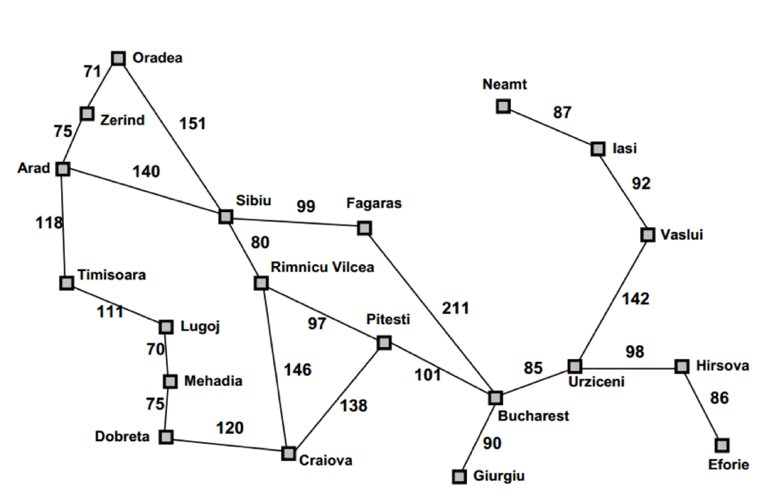
\includegraphics[width=0.7\textwidth]{apendices/fig/1_IAA001_1.png} 
        \caption*{Fonte: IAA UFPR (2024).}
        %\label{fig:minha_figura}
    \end{figure}
    \begin{figure}[H]
        \centering
        \caption{Distâncias em linha reta para a cidade de Bucharest}
        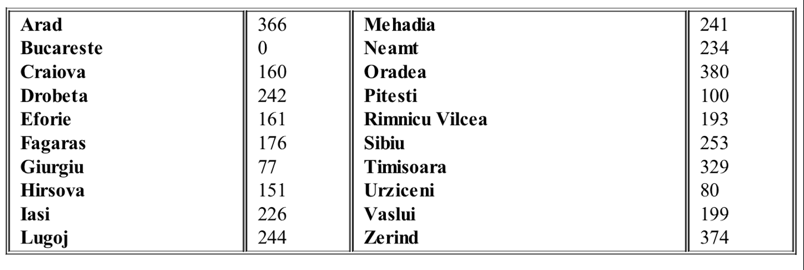
\includegraphics[width=0.7\textwidth]{apendices/fig/1_IAA001_2.png} 
        \caption*{Fonte: IAA UFPR (2024).}
        %\label{fig:minha_figura}
    \end{figure}

\subsection*{\textbf{3 Lógica}}
    Verificar se o argumento lógico é válido.

    \begin{adjustwidth}{3em}{}
        \begin{quote}
            \itshape
            Se as uvas caem, então a raposa as come \\
            Se a raposa as come, então estão maduras \\
            As uvas estão verdes ou caem

            Logo

            A raposa come as uvas se e somente se as uvas caem
        \end{quote}
    \end{adjustwidth}

    Deve ser apresentada uma prova, no mesmo formato mostrado nos conteúdos de aula e nas práticas.

    \begin{adjustwidth}{1em}{}
    \textbf{Dicas:}
    \end{adjustwidth}
    \begin{enumerate}[label=\arabic*.]
        \item Transformar as afirmações para lógica:

        $p$: as uvas caem \\
        $q$: a raposa come as uvas \\
        $r$: as uvas estão maduras

        \item Transformar as três primeiras sentenças para formar a base de conhecimento

        R1: $p \rightarrow q$ \\
        R2: $q \rightarrow r$ \\
        R3: $\neg r \vee p$

        \item Aplicar equivalências e regras de inferência para se obter o resultado esperado. Isto é, com essas três primeiras sentenças devemos derivar $q \leftrightarrow p$. Cuidado com a ordem em que as fórmulas são geradas.

        \textbf{Equivalência Implicação:} $(\alpha \rightarrow \beta)$ equivale a $(\neg \alpha \vee \beta)$

        \textbf{Silogismo Hipotético:} $\alpha \rightarrow \beta$, $\beta \rightarrow \gamma \vdash \alpha \rightarrow \gamma$

        \textbf{Conjunção:} $\alpha$, $\beta \vdash \alpha \wedge \beta$

        \textbf{Equivalência Bicondicional:} $(\alpha \leftrightarrow \beta)$ equivale a $(\alpha \rightarrow \beta) \wedge (\beta \rightarrow \alpha)$
    \end{enumerate}

    \begin{enumerate}[label=\alph*)]
        \item \textbf{(25 pontos)} Deve-se mostrar todos os passos e regras aplicadas, no mesmo formato apresentado nas aulas e nas práticas. As equivalências e regras necessárias estão descritas acima e no material.
    \end{enumerate}

\subsection*{\textbf{4 Redes Neurais Artificiais}}
    Seja a RNA da figura abaixo.
    
    \begin{figure}[H]
        \centering
        \caption{Rede Neural Artificial exercício 4}
        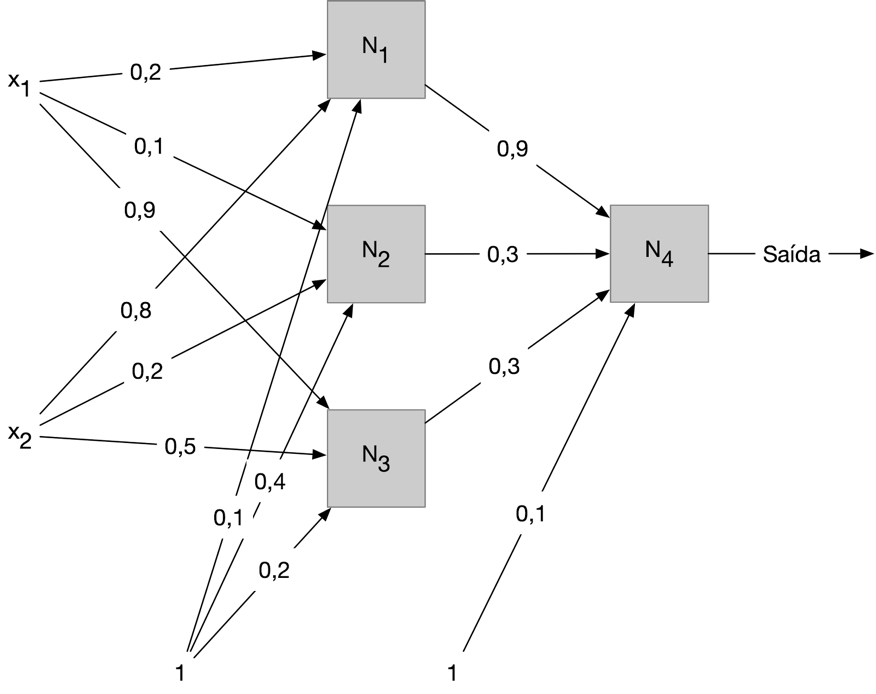
\includegraphics[width=0.7\textwidth]{apendices/fig/1_IAA001_3.png} 
        \caption*{Fonte: IAA UFPR (2024).}
        %\label{fig:minha_figura}
    \end{figure}

    Os neurônios $N_1$, $N_2$ e $N_3$ possuem função de ativação linear. Já $N_4$ possui função de ativação tangente hiperbólica (pesquise a fórmula e aplique).

    Dada a entrada $x_1 = -3$, $x_2 = 1$, dê:
    \begin{enumerate}[label=\alph*)]
        \item \textbf{(6,25 pontos)} Valor de saída do neurônio N1
        \item \textbf{(6,25 pontos)} Valor de saída do neurônio N2
        \item \textbf{(6,25 pontos)} Valor de saída do neurônio N3
        \item \textbf{(6,25 pontos)} Valor de saída da rede como um todo
    \end{enumerate}

\section*{\textbf{B - RESOLUÇÃO}}
\setcounter{subsection}{0}

\subsection*{\textbf{1 ChatGPT}}
\begin{adjustwidth}{1em}{}
\textbf{a) Pergunte ao ChatGPT o que é Inteligência Artificial e cole aqui o resultado.}
\end{adjustwidth}

Inteligência Artificial (IA) refere-se à capacidade de um sistema ou programa de computador realizar tarefas que normalmente exigiriam inteligência humana. Essas tarefas incluem raciocínio, aprendizado, percepção visual, reconhecimento de fala, compreensão de linguagem natural, tomada de decisões e resolução de problemas.

Os sistemas de IA são projetados para imitar certos aspectos da inteligência humana, utilizando algoritmos e modelos matemáticos para processar dados, aprender padrões e tomar decisões. Existem dois tipos principais de IA:

\begin{enumerate}
    \item IA Fraca (ou Estreita): Refere-se a sistemas de IA especializados em tarefas específicas. Eles são limitados ao escopo de suas programações e não têm a capacidade de realizar tarefas além do que foram projetados para fazer. Exemplos incluem reconhecimento de voz, chatbots e carros autônomos.
    \item IA Forte (ou Geral): Envolve sistemas que têm a capacidade de realizar qualquer tarefa cognitiva que um ser humano pode fazer. Este nível de IA ainda não foi totalmente alcançado e é um campo de pesquisa em desenvolvimento.
\end{enumerate}
    
Algoritmos de aprendizado de máquina (Machine Learning) são frequentemente usados na implementação de sistemas de IA. Eles permitem que a IA melhore seu desempenho em uma tarefa específica à medida que é exposta a mais dados, sem ser explicitamente programada.

A Inteligência Artificial tem aplicações em uma variedade de setores, como medicina, finanças, automação industrial, reconhecimento de padrões, entretenimento e muito mais. É uma área de rápido avanço e continua a desempenhar um papel significativo na transformação de várias indústrias.

\begin{adjustwidth}{1em}{}
\textbf{b) Dada essa resposta do ChatGPT, classifique usando as 4 abordagens vistas em
sala. Explique o porquê.}
\end{adjustwidth}

A definição dada pelo ChatGPT menciona que sistemas de Inteligência Artificial são projetados para "imitar certos aspectos da inteligência humana", o que parece se assemelhar mais à definição de Pensar como Humanos ou Agir como Humanos.

\begin{adjustwidth}{1em}{}
\textbf{c) Pesquise sobre o funcionamento do ChatGPT (sem perguntar ao próprio
ChatGPT) e escreva um texto contendo no máximo 5 parágrafos. Cite as referências.}
\end{adjustwidth}

O ChatGPT pode se entendido como uma extrapolação de uma classe de modelos de aprendizagem de máquina chamados Large Language Models (LLMs), que são modelos de Processamento de Linguagem Natural. Esse tipo de modelo consegue processar grandes quantidades de texto e inferir relações entre palavras dentro do texto. A capacidade dos LLMs cresce conforme aumenta o tamanho e variedade de parâmetros da base de dados.\cite{towardsdatascience}

Segundo o que é disponibilidado pelo OpenAI\cite{OpenAI}, ele é baseado na arquitetura GPT (Generative Pre-trained Transformer), um modelo Transformer, que é uma rede neural capaz de aprender o contexto dado e gerar um novo texto a partir disso. A rede foi otimizada para usar um método de treinamento chamado Reinforcement Learning with Human Feedback (RLHF), que usa demonstrações humanas para guiar seu comportamento, de forma a alcançar o desejável.

Segundo Rama Ramakrishnan, professor do MIT, \cite{MIT}, o modelo precedente, GPT-3, foi treinado com cerca de 30 bilhões de frases retiradas de livros e da internet, para uma única tarefa: prever a palavra seguinte em uma frase, dadas as palavras usadas anteriormente. Ele calcula uma tabela de probabilidades para possíveis palavras a serem usadas e usa a que tem a melhor probabilidade, quase como um sistema de \textit{autocomplete}. Para formar frases completas, a cada palavra escolhida, ele adiciona ela à frase e refaz o processo de cálculo das probabilidades para escolher a próxima palavra. Já a versão 3.5 foi treinada para seguir instruções dadas por humanos, utilizando uma base de dados contendo pares de exemplos de instruções e respostas de alta qualidade para tais instruções. O modelo treinado a partir dessa base de dados foi então utilizado para gerar múltiplas respostas para cada uma das instruções e essas respostas foram categorizadas por humanos de mais útil a menos útil. A partir desses novos dados, foi possível treinar um "modelo de recompensa", que avalia a qualidade das respostas geradas pelo GPT-3.5 e retorna uma "nota" de avaliação para o GPT-3.5, assim ele passa por um \textit{fine tuning} para melhorar suas respostas com \textit{reinforcement learning}. Na transição do GPT-3.5 para o ChatGPT foi usado um processo similar, mas desta vez utilizando conversas inteiras para o treinamento.

Ele é treinado usando textos escritos por humanos, incluindo conversações, de forma a conseguir imitar o estilo de comunicação humano). Assim, de acordo com os dados utilizados para treinamento, ele pode, inclusive, produzir textos com conteúdo enviesado.

\begin{adjustwidth}{1em}{}
\textbf{d) Entendendo o que é o ChatGPT, classifique o próprio ChatGPT usando as 4
abordagens vistas em sala. Explique o porquê.}
\end{adjustwidth}

De acordo com o comportamento, que se baseia em aprender e imitar como humanos se comunicam, ele parece se encaixar na definição da abordagem Agir como Humanos. Essa conclusão pode ser atingida considerando-se que o ChatGPT encontra padrões nos textos, que são dados produzidos (majoritariamente) por humanos, e com isso aprende contextos, mas não é totalmente consciente sobre o seu conteúdo, e não usa um processo cognitivo, apenas os sintetiza conforme foram fornecidos a ele. Como exemplo, se o ChatGPT fosse treinado com textos com um viés racista, ele poderia reproduzir textos racistas, já que não tem a capacidade de ponderar se racismo é correto ou não de um ponto de vista racional, ou seja, ele não toma decisões racionais baseadas no contexto que é apresentado a ele, apenas busca imitar a forma como humanos se comunicam.

\subsection*{\textbf{2 Busca Heurística}}
%\begin{figure}[H]
%\centering
%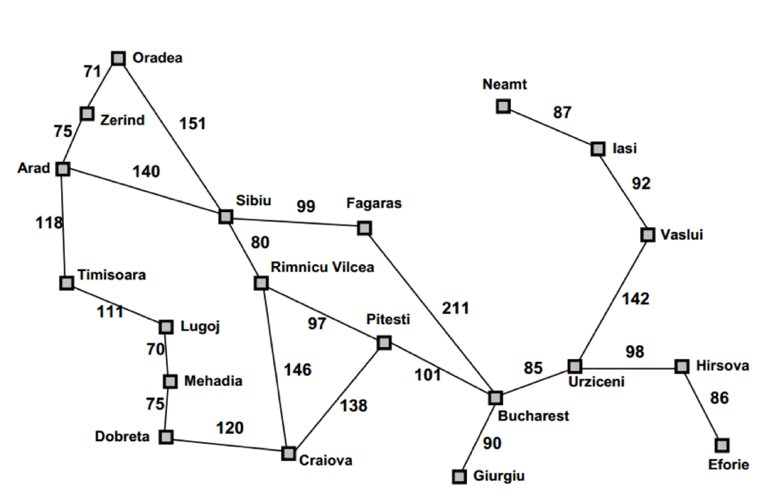
\includegraphics[width=0.6\linewidth]{apendices/fig/1_IAA001_1.png}
%\caption{Rotas Lugoj-Bucharest}
%\label{grafoAStar}
%\end{figure}

\begin{adjustwidth}{1em}{}
\textbf{a) Apresente a árvore final, contendo os valores, da mesma forma que foi apresentado
na disciplina e nas práticas. Use o formato de árvore, não será permitido um formato em blocos,
planilha, ou qualquer outra representação.}
\end{adjustwidth}

\begin{figure}[H]
\centering
\caption{Árvore final}
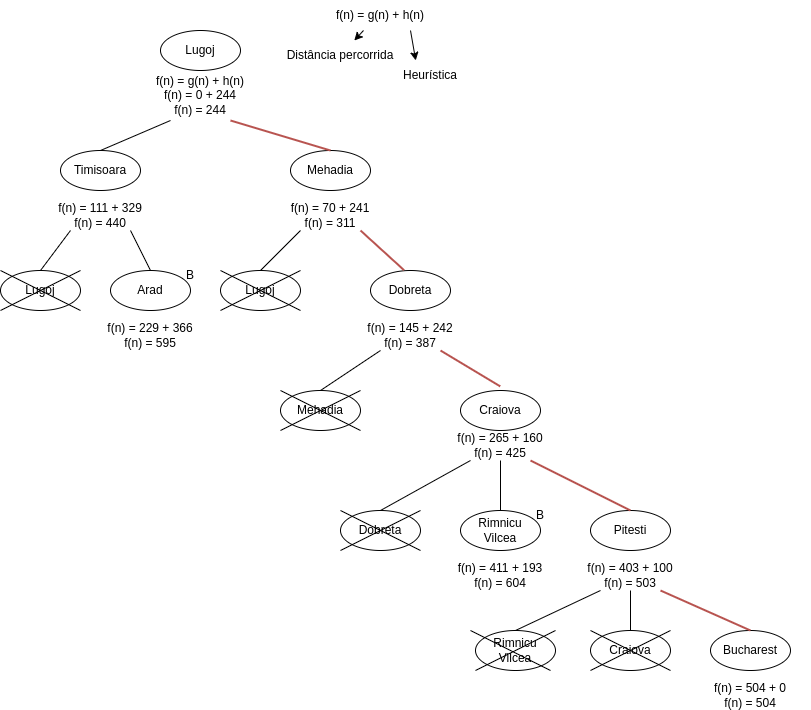
\includegraphics[width=0.8\linewidth]{apendices/fig/1_IAA001_4.png}
\caption*{Fonte: O autor (2024).}
\label{arvoreF}
\end{figure}

$Lugoj \Rightarrow Mehadia \Rightarrow Dobreta \Rightarrow Craiova \Rightarrow Pitesti \Rightarrow Bucharest$ = 504

\subsection*{\textbf{3 Lógica}}
\begin{adjustwidth}{3em}{}
\begin{quote}
    \itshape
    Se as uvas caem, então a raposa as come \\
    Se a raposa as come, então estão maduras \\
    As uvas estão verdes ou caem

    Logo

    A raposa come as uvas se e somente se as uvas caem
\end{quote}
\end{adjustwidth}

$p$: as uvas caem 

$q$: a raposa come as uvas 

$r$: as uvas estão maduras

\begin{equation*}
    \begin{gathered}
        R1: p \Rightarrow q \\
        R2: q \Rightarrow r \\
        R3: \neg{r} \lor p \\
    \end{gathered}
\end{equation*}

objetivo: 
\begin{equation*}
    q \Leftrightarrow p
\end{equation*}

%ou seja, aplicando a Equivalência Bicondicional:

%\begin{equation*}
%    p \Rightarrow q \ e \ q \Rightarrow p
%\end{equation*}

\begin{adjustwidth}{1em}{}
\textbf{a) Deve-se mostrar todos os passos e regras aplicadas, no mesmo formato
apresentado nas aulas e nas práticas.}
\end{adjustwidth}

%Como a primeira afirmação lógica necessária para a prova já está na base de conhecimento (R1), para que a equivalência acima seja verdadeira, é necessário provar que:

%\begin{equation*}
%    q \Rightarrow p
%\end{equation*}

%Partindo da base de conhecimento:

% de \ R1 \ e \ R2:
% \begin{equation}
%     R4: p \Rightarrow r \\
% \end{equation}

%usando Equivalência Implicação em R3 temos:

\begin{equation*}
    \begin{gathered}
        R1: p \Rightarrow q \\
        R2: q \Rightarrow r \\
        R3: \neg{r} \lor p \\
    \end{gathered}
\end{equation*}

%\hrule

\begin{align*}
    R4: r \Rightarrow p && \text{Equivalência Implicação, R3 }
\end{align*}
%usando Silogismo Hipotético em R2 e R4, temos que:
\begin{align*}
    R5: q \Rightarrow p && \text{SH, R2, R4 }
\end{align*}
\begin{align*}
    R6: p \Rightarrow q \land q \Rightarrow p && \text{CONJ, R1, R5 }
\end{align*}
\begin{align*}
    R7: q \Leftrightarrow p && \text{BICOND, R6 }
\end{align*}

%concluindo assim a prova lógica.

\subsection*{\textbf{4 Redes Neurais Artificiais}}

x1=-3, x2=1

N1, N2, N3: função de ativação linear (mantém o valor)

N4: função de ativação tangente (produz valores no intervalo [-1,1])

\begin{figure}[!h]
\centering
\caption{Tangente Hiperbólica}
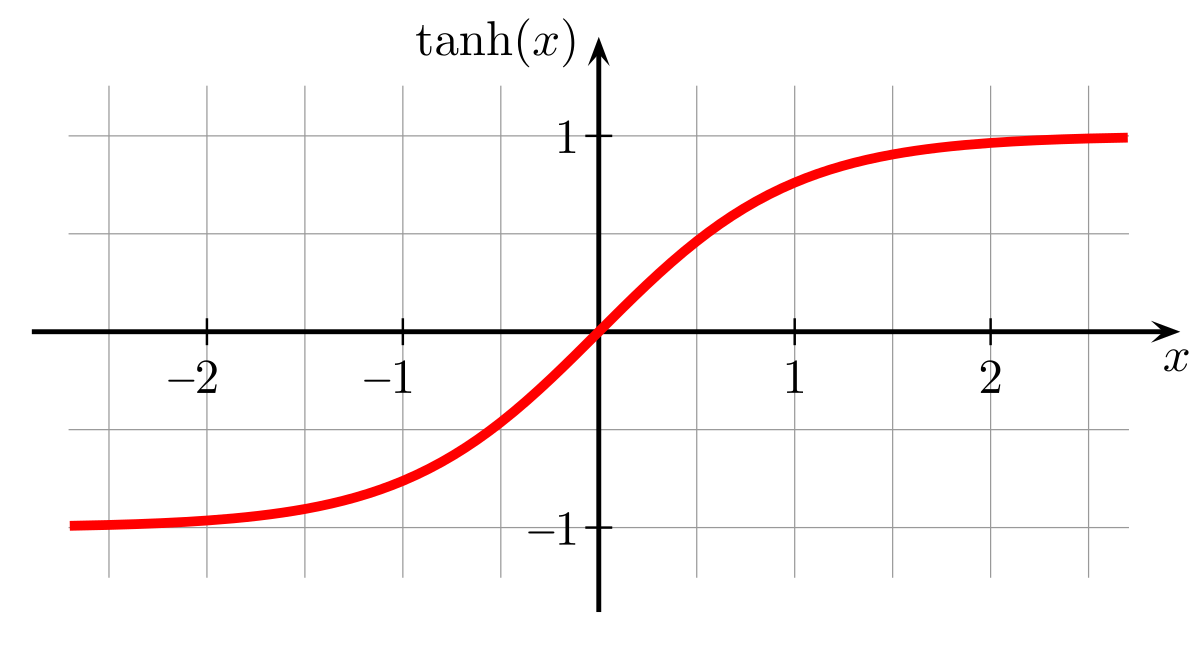
\includegraphics[width=0.6\linewidth]{apendices/fig/1_IAA001_5.png}
\caption*{Fonte: O autor (2024).}
\label{tanh}
\end{figure}

%\begin{figure}[H]
%\centering
%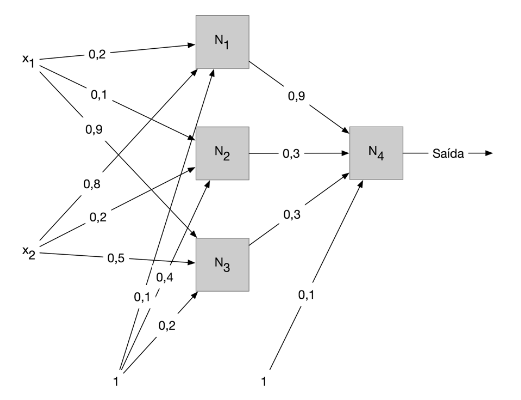
\includegraphics[width=0.6\linewidth]{apendices/fig/1_IAA001_6.png}
%\caption{Rede Neural Artificial exercício 4}
%\label{rede}
%\end{figure}

\begin{adjustwidth}{1em}{}
\textbf{a) Valor de saída do neurônio N1}
\end{adjustwidth}
\begin{equation*}
    (-3)\times0.2 + 1\times0.8 + 1\times0.1 = 0.3
\end{equation*}

\begin{adjustwidth}{1em}{}
\textbf{b) Valor de saída do neurônio N2}
\end{adjustwidth}
\begin{equation*}
    (-3)\times0.1 + 1\times0.2 + 1\times0.4 = 0.3
\end{equation*}

\begin{adjustwidth}{1em}{}
\textbf{c) Valor de saída do neurônio N3}
\end{adjustwidth}
\begin{equation*}
    (-3)\times0.9 + 1\times0.5 + 1\times0.2 = -2
\end{equation*}

\begin{adjustwidth}{1em}{}
\textbf{d) Valor de saída da rede como um todo}
\end{adjustwidth}
\begin{equation*}
    tanh(0.3\times0.9 + 0.3\times0.3 + (-2)\times0.3 + 1\times0.1) = tanh(0.27 + 0.09 - 0.6 + 0.1) = -0.13909 \approx -0.14
\end{equation*}
\label{ap:ap02}
\chapter{Linguagem de Programação Aplicada}

\section*{\textbf{A - ENUNCIADO}}
\textbf{Nome da base de dados do exercício}: \textit{precos\_carros\_brasil.csv}

\textbf{Informações sobre a base de dados: }

Dados dos preços médios dos carros brasileiros, das mais diversas marcas, no ano de 2021, de acordo com dados extraídos
da tabela FIPE (Fundação Instituto de Pesquisas Econômicas). A base original foi extraída do site Kaggle
(\href{https://www.kaggle.com/datasets/vagnerbessa/average-car-prices-bazil/data}{\textcolor[HTML]{1155CC}{Acesse aqui
a base original}}). A mesma foi adaptada para ser utilizada no presente exercício.

Observação: As variáveis \textit{fuel\hspace{0pt}\hspace{0pt}}, \textit{gear} e \textit{engine\_size} foram extraídas
dos valores da coluna \textit{model}, pois na base de dados original não há coluna dedicada a esses valores. Como
alguns valores do modelo não contêm as informações do tamanho do motor, este conjunto de dados não contém todos os
dados originais da tabela FIPE.

\textbf{Metadados:}
\begin{table}[H]
\centering
\caption{Metadados da Tabela FIPE}
\begin{tabular}{|p{0.4\textwidth}|p{0.55\textwidth}|}
\hline
\textbf{Nome do campo} & \textbf{Descrição} \\
\hline
year\_of\_reference & O preço médio corresponde a um mês do ano de referência \\
\hline
month\_of\_reference & O preço médio corresponde a um mês específico, pois a FIPE atualiza mensalmente \\
\hline
fipe\_code & Código único da FIPE \\
\hline
authentication & Código único de autenticação para consulta FIPE \\
\hline
brand & Marca do carro \\
\hline
model & Modelo do carro \\
\hline
fuel & Tipo de combustível \\
\hline
gear & Tipo de engrenagem \\
\hline
engine\_size & Tamanho do motor em centímetros cúbicos \\
\hline
year\_model & Ano do modelo (pode ser diferente do ano de fabricação) \\
\hline
avg\_price & Preço médio do carro em reais \\
\hline
\end{tabular}
\caption*{Fonte: IAA UFPR (2024).}
\end{table}



\textbf{\textit{Atenção: ao fazer o download da base de dados, selecione o formato .csv. É o formato que será
considerado correto na resolução do exercício.}}



\newpage
\subsection*{\textbf{1 Análise Exploratória dos dados}}
%\textbf{1 Análise Exploratória dos dados}



A partir da base de dados \textbf{precos\_carros\_brasil.csv}, execute as seguintes tarefas:

\begin{enumerate}[series=listWWNumxi,label=\alph*.,ref=\alph*]
\item Carregue a base de dados media\_precos\_carros\_brasil.csv
\item Verifique se há valores faltantes nos dados. Caso haja, escolha uma tratativa para resolver o problema de valores
faltantes
\item Verifique se há dados duplicados nos dados
\item Crie duas categorias, para separar colunas numéricas e categóricas. Imprima o resumo de informações das variáveis
numéricas e categóricas (estatística descritiva dos dados)
\item Imprima a contagem de valores por modelo (model) e marca do carro (brand)
\item Dê um breve explicação (máximo de quatro linhas) sobre os principais resultados encontrados na Análise
Exploratória dos dados
\end{enumerate}


\subsection*{\textbf{2 Visualização dos dados}}
%\textbf{2 Visualização dos dados}

A partir da base de dados \textbf{precos\_carros\_brasil.csv,} execute as seguintes tarefas:

\begin{enumerate}[series=listWWNumx,label=\alph*.,ref=\alph*]
\item Gere um gráfico da distribuição da quantidade de carros por marca
\item Gere um gráfico da distribuição da quantidade de carros por tipo de engrenagem do carro
\item Gere um gráfico da evolução da média de preço dos carros ao longo dos meses de 2022 (variável de tempo no eixo X)
\item Gere um gráfico da distribuição da média de preço dos carros por marca e tipo de engrenagem
\item Dê uma breve explicação (máximo de quatro linhas) sobre os resultados gerados no item d
\item Gere um gráfico da distribuição da média de preço dos carros por marca e tipo de combustível
\item Dê uma breve explicação (máximo de quatro linhas) sobre os resultados gerados no item f
\end{enumerate}






\subsection*{\textbf{3 Aplicação de modelos de machine learning para prever o preço médio dos carros}}
%\textbf{3 Aplicação de modelos de machine learning para prever o preço médio dos carros}




{\centering
A partir da base de dados \textbf{precos\_carros\_brasil.csv}, execute as seguintes tarefas:
\par}

\begin{enumerate}[series=listWWNumxii,label=\alph*.,ref=\alph*]
\item Escolha as variáveis \textbf{numéricas} (modelos de Regressão) para serem as variáveis independentes do modelo.A
variável target é \textbf{avg\_price. Observação:} caso julgue necessário, faça a transformação de variáveis
categóricas em variáveis numéricas para inputar no modelo. Indique \textbf{quais variáveis} foram transformadas e
\textbf{como} foram transformadas
\item Crie partições contendo 75\% dos dados para treino e 25\% para teste
\item Treine modelos RandomForest (biblioteca RandomForestRegressor) e XGBoost (biblioteca XGBRegressor) para predição
dos preços dos carros. \textbf{Observação}: caso julgue necessário, mude os parâmetros dos modelos e rode novos
modelos. Indique quais parâmetros foram inputados e indique o treinamento de cada modelo
\item Grave os valores preditos em variáveis criadas
\item Realize a análise de importância das variáveis para estimar a variável target, \textbf{para cada modelo treinado}
\item Dê uma breve explicação (máximo de quatro linhas) sobre os resultados encontrados na análise de importância de
variáveis
\item Escolha o melhor modelo com base nas métricas de avaliação MSE, MAE e R²
\item Dê uma breve explicação (máximo de quatro linhas) sobre qual modelo gerou o melhor resultado e a métrica de
avaliação utilizada
\end{enumerate}

\section*{\textbf{B - RESOLUÇÃO}}

\subsection*{\textbf{1 Análise Exploratória dos dados}}
\begin{adjustwidth}{1em}{}
\textbf{a. Carregue a base de dados media\_precos\_carros\_brasil.csv}
\end{adjustwidth}

\begin{lstlisting}[language=Python, style=input]
# Para rápida instalação das bibliotecas necessárias, rodar o script abaixo no CLI:
# pip install -r requirements.txt

import pandas as pd
import seaborn as sns
import matplotlib.pyplot as plt
import numpy as np

import warnings
warnings.filterwarnings('ignore')

from sklearn.model_selection import train_test_split
from sklearn.ensemble import RandomForestRegressor
from xgboost import XGBRegressor
from sklearn.preprocessing import LabelEncoder
from sklearn.model_selection import RandomizedSearchCV

# Métricas de avaliação dos modelos
from sklearn.metrics import mean_squared_error, mean_absolute_error, r2_score

dados = pd.read_csv('precos_carros_brasil.csv')
dados.head()
\end{lstlisting}


\begin{table}[H]
\centering
\begin{tcolorbox}[myoutputstyle, width=1.1\textwidth, enlarge left by=-1cm]
%\resizebox{\textwidth}{!}{ % scales table to fit page width
\renewcommand{\arraystretch}{1.2} % more vertical space in rows
\setlength{\tabcolsep}{6pt} % adjust horizontal padding between columns
\resizebox{0.95\textwidth}{!}{
\begin{tabular}{lllllllllll}
\textbf{year\_ref} & \textbf{month} & \textbf{fipe\_code} & \textbf{auth} & \textbf{brand} & \textbf{model} & \textbf{fuel} & \textbf{gear} & \textbf{engine} & \textbf{year} & \textbf{price} \\
\hline
2021.0 & January & 004001-0 & cfzlctzfwrcp & GM - Chevrolet & Corsa Wind 1.0 MPFI / EFI 2p & Gasoline & manual & 1 & 2002.0 & 9162.0 \\
2021.0 & January & 004001-0 & cdqwxwpw3y2p & GM - Chevrolet & Corsa Wind 1.0 MPFI / EFI 2p & Gasoline & manual & 1 & 2001.0 & 8832.0 \\
2021.0 & January & 004001-0 & cb1t3xwwj1xp & GM - Chevrolet & Corsa Wind 1.0 MPFI / EFI 2p & Gasoline & manual & 1 & 2000.0 & 8388.0 \\
2021.0 & January & 004001-0 & cb9gct6j65r0 & GM - Chevrolet & Corsa Wind 1.0 MPFI / EFI 2p & Alcohol  & manual & 1 & 2000.0 & 8453.0 \\
2021.0 & January & 004003-7 & g15wg0gbz1fx & GM - Chevrolet & Corsa Pick-Up GL/ Champ 1.6 MPFI / EFI & Gasoline & manual & 1.6 & 2001.0 & 12525.0 \\
\end{tabular}
}
\end{tcolorbox}
%\caption{Sample data output from DataFrame}
\end{table}

\begin{adjustwidth}{1em}{}
\textbf{b. Verifique se há valores faltantes nos dados. Caso haja, escolha uma tratativa para resolver o problema de valores faltantes}
\end{adjustwidth}

\begin{lstlisting}[language=Python, style=input]
# Excluindo as linhas sem dados (caracteristica de importacao de .CSV)
dados = dados.dropna(how='all')

antes = dados.shape

# Verificando se existem valores faltantes nos dados 
dados.isna().any()
\end{lstlisting}
\begin{lstlisting}[language=, style=output]
year_of_reference     False
month_of_reference    False
fipe_code             False
authentication        False
brand                 False
model                 False
fuel                  False
gear                  False
engine_size           False
year_model            False
avg_price_brl         False
dtype: bool
\end{lstlisting}
Não há valores faltantes.


\begin{adjustwidth}{1em}{}
\textbf{c. Verifique se há dados duplicados nos dados}
\end{adjustwidth}


\begin{lstlisting}[language=Python, style=input]
# Verificando se temos valores duplicados
dados.duplicated().sum() 
\end{lstlisting}
\begin{lstlisting}[language=, style=output]
2
\end{lstlisting}

\begin{lstlisting}[language=Python, style=input]
# Removendo valores duplicados
dados.drop_duplicates(inplace=True)

depois = dados.shape

# Verifica diferença após a normalização dos dados
diff_linhas =  depois[0] - antes[0]
diff_colunas = depois[1] - antes[1]
print("Linhas:\n Antes {} x Depois {} = Diff {}".format(antes[0], depois[0], diff_linhas))
print("Colunas:\n Antes {} x Depois {} = Diff {}".format(antes[1], depois[1], diff_colunas))
\end{lstlisting}
\begin{lstlisting}[language=, style=output]
Linhas:
 Antes 202297 x Depois 202295 = Diff -2
Colunas:
 Antes 11 x Depois 11 = Diff 0
\end{lstlisting}

2 linhas duplicadas excluídas.

\begin{adjustwidth}{1em}{}
\textbf{d. Crie duas categorias, para separar colunas numéricas e categóricas. Imprima o resumo de informações das variáveis numéricas e categóricas (estatística descritiva dos dados)}
\end{adjustwidth}

\begin{lstlisting}[language=Python, style=input]
# Criando categorias para separar colunas numéricas e categóricas: facilita a AED
numericas_cols = [col for col in dados.columns if dados[col].dtype != 'object']
categoricas_cols = [col for col in dados.columns if dados[col].dtype == 'object']

# Resumo das variáveis numéricas - Imprime alguns valores de medidas de tendências centrais 
dados[numericas_cols].describe()
\end{lstlisting}
\begin{table}[H]
\centering
\begin{tcolorbox}[myoutputstyle]
\begin{tabular}{lrrr}
\hline
 & \textbf{year\_of\_reference} & \textbf{year\_model} & \textbf{avg\_price\_brl} \\
\hline
count & 202295.000000 & 202295.000000 & 202295.000000 \\
mean & 2021.564695 & 2011.271514 & 52756.765713 \\
std  & 0.571904 & 6.376241 & 51628.912116 \\
min  & 2021.000000 & 2000.000000 & 6647.000000 \\
25\% & 2021.000000 & 2006.000000 & 22855.000000 \\
50\% & 2022.000000 & 2012.000000 & 38027.000000 \\
75\% & 2022.000000 & 2016.000000 & 64064.000000 \\
max  & 2023.000000 & 2023.000000 & 979358.000000 \\
\hline
\end{tabular}
\end{tcolorbox}
%\caption{Descriptive statistics for vehicle data}
%\label{tab:vehicle_stats}
\end{table}

\begin{adjustwidth}{1em}{}
\textbf{e. Imprima a contagem de valores por modelo (model) e marca do carro (brand)}
\end{adjustwidth}
\begin{lstlisting}[language=Python, style=input]
# Contagem de valores por categoria de 'Modelo'
dados['model'].value_counts()
\end{lstlisting}
\begin{lstlisting}[language=, style=output]
Palio Week. Adv/Adv TRYON 1.8 mpi Flex    425
Focus 1.6 S/SE/SE Plus Flex 8V/16V 5p     425
Focus 2.0 16V/SE/SE Plus Flex 5p Aut.     400
Saveiro 1.6 Mi/ 1.6 Mi Total Flex 8V      400
Corvette 5.7/ 6.0, 6.2 Targa/Stingray     375
                                         ... 
STEPWAY Zen Flex 1.0 12V Mec.               2
Saveiro Robust 1.6 Total Flex 16V CD        2
Saveiro Robust 1.6 Total Flex 16V           2
Gol Last Edition 1.0 Flex 12V 5p            2
Polo Track 1.0 Flex 12V 5p                  2
Name: model, Length: 2112, dtype: int64
\end{lstlisting}
\begin{lstlisting}[language=Python, style=input]
# Contagem de valores por categoria de 'Marca'
dados['brand'].value_counts()
\end{lstlisting}
\begin{lstlisting}[language=, style=output]
Fiat               44962
VW - VolksWagen    44312
GM - Chevrolet     38590
Ford               33150
Renault            29191
Nissan             12090
Name: brand, dtype: int64
\end{lstlisting}

\begin{adjustwidth}{1em}{}
\textbf{f. Dê um breve explicação (máximo de quatro linhas) sobre os principais resultados encontrados na Análise Exploratória dos dados}
\end{adjustwidth}
Na Análise Exploratória dos Dados pudemos observar que o conjunto de dados possui 11 colunas e nenhuma delas possui dados faltantes. Ao observarmos valores duplicados, apenas 2 linhas estavam duplicadas. Das 11 colunas, apenas 3 são numéricas. Porém, as colunas brand e model podem ser facilmente convertidas para númericas.

\subsection*{\textbf{2 Visualização dos dados}}
\begin{adjustwidth}{1em}{}
\textbf{a. Gere um gráfico da distribuição da quantidade de carros por marca}
\end{adjustwidth}
\begin{lstlisting}[language=Python, style=input]
# Gráfico da distribuição por marca
plt.figure(figsize=(20,10)) 
plt.bar(dados['brand'].unique(), dados['brand'].value_counts()) 
plt.title('Distribuição de carros por marca') 
plt.ylabel('Total de carros') 
plt.xlabel('Marca') 
\end{lstlisting}
\begin{figure}[H]
\centering
\caption{Distribuição de carros por marca}
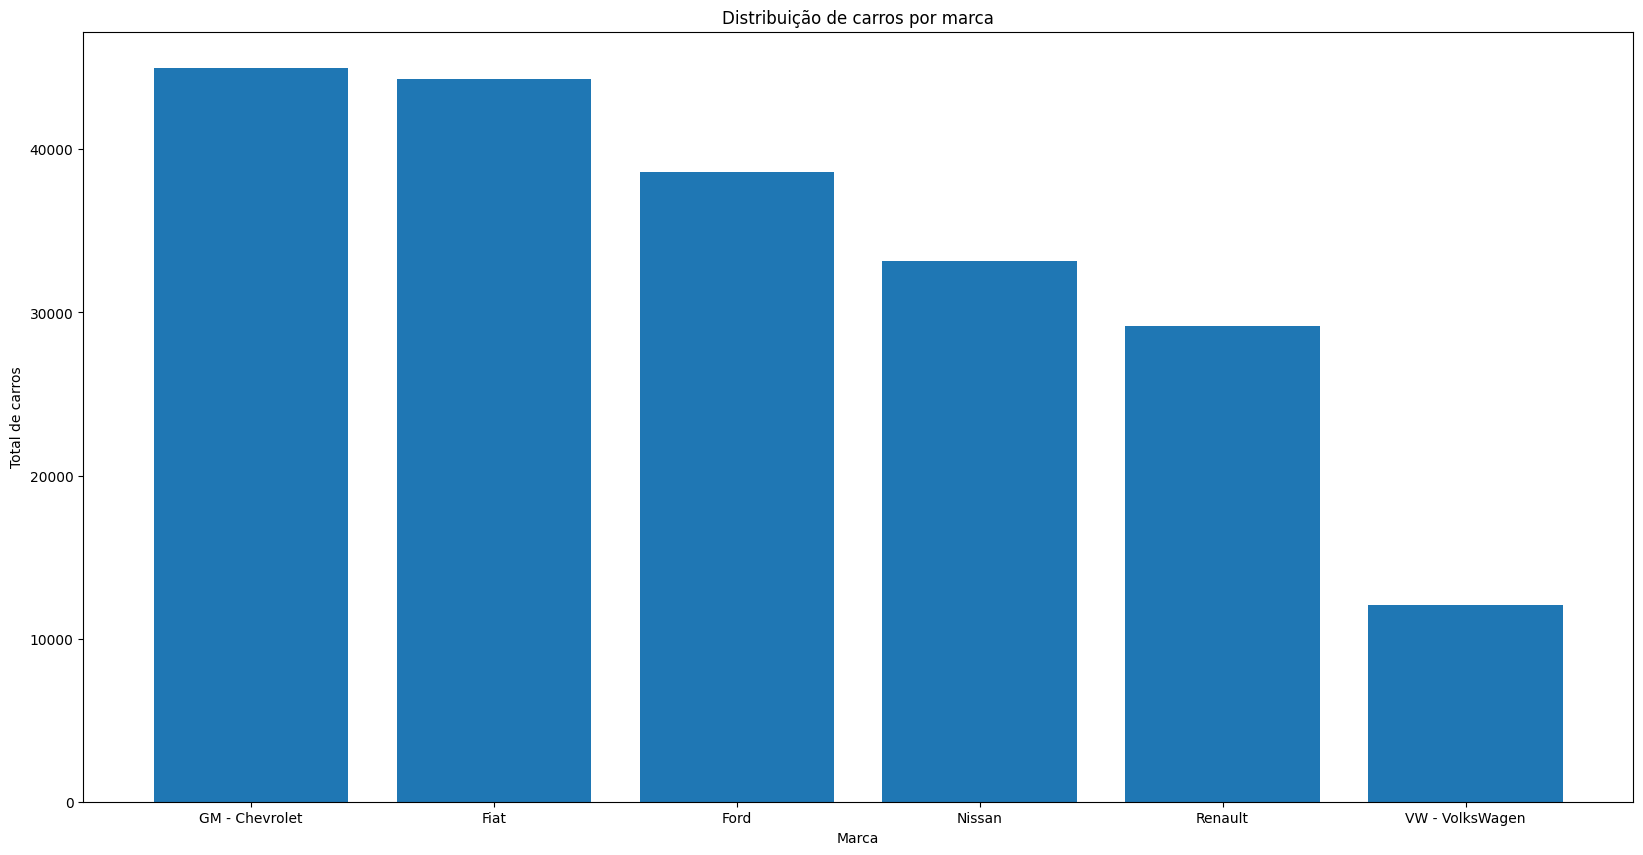
\includegraphics[width=1\linewidth]{apendices/fig/2_IAA002_1.png}
\caption*{Fonte: O autor (2024).}
\end{figure}

\begin{adjustwidth}{1em}{}
\textbf{b. Gere um gráfico da distribuição da quantidade de carros por tipo de engrenagem do carro}
\end{adjustwidth}
\begin{lstlisting}[language=Python, style=input]
# Gráfico da distribuição por engrenagem (tipo de marcha)
plt.figure(figsize=(20,10)) 
plt.bar(dados['gear'].unique(), dados['gear'].value_counts()) 
plt.title('Distribuição de carros por engrenagem (marcha)') 
plt.ylabel('Total de carros') 
plt.xlabel('Tipo de engrenagem (marcha)') 
\end{lstlisting}
\begin{figure}[H]
\centering
\caption{Distribuição de carros por engrenagem (marcha)}
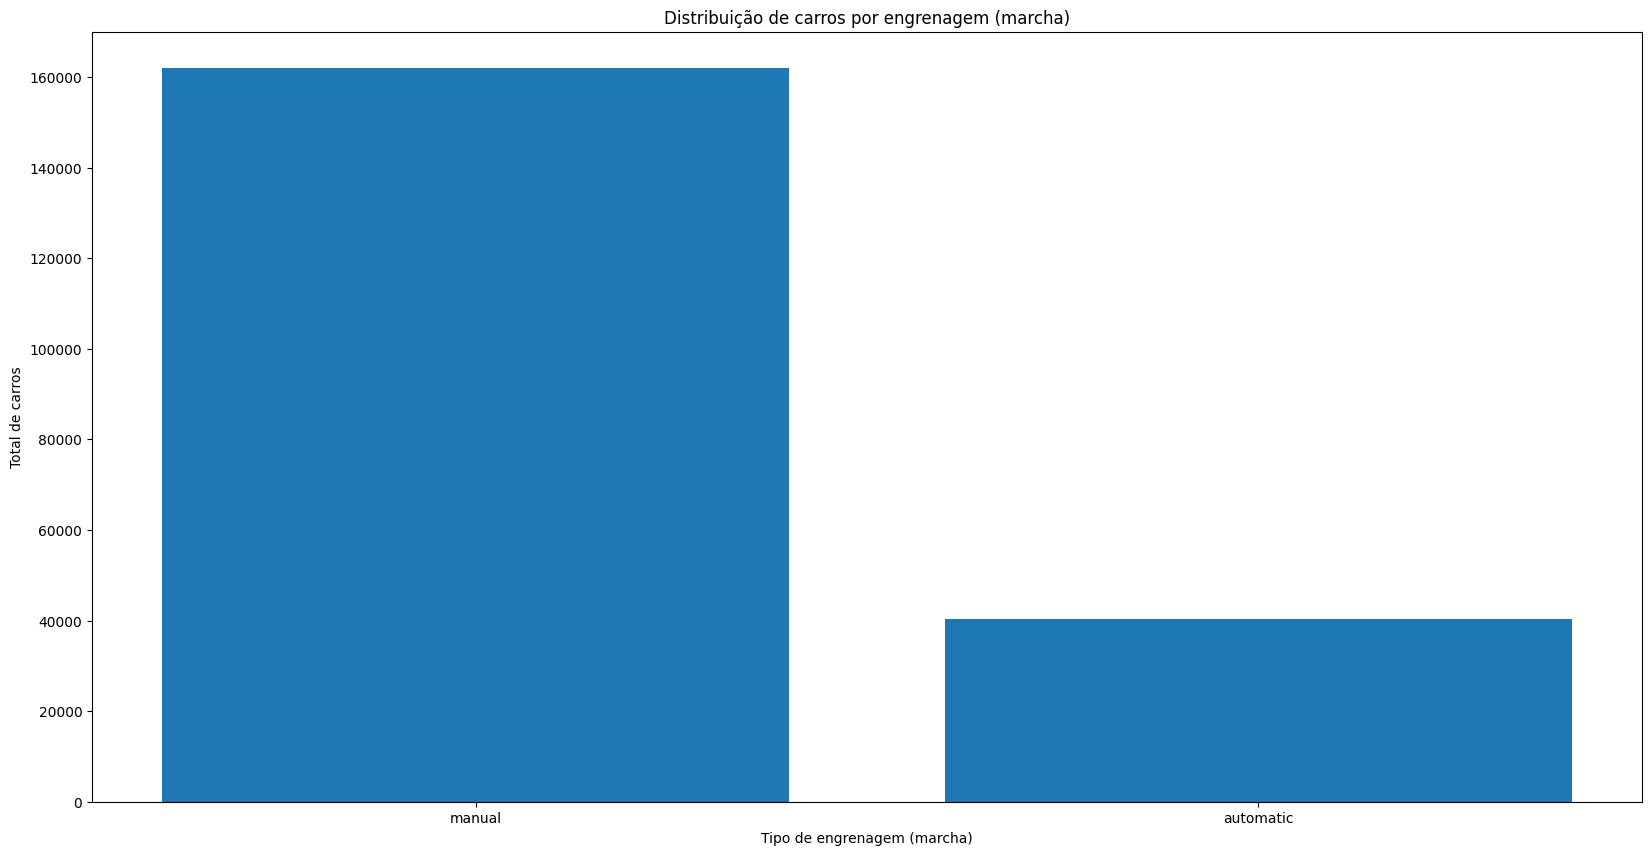
\includegraphics[width=1\linewidth]{apendices/fig/2_IAA002_2.png}
\caption*{Fonte: O autor (2024).}
\end{figure}

\begin{adjustwidth}{1em}{}
\textbf{c. Gere um gráfico da evolução da média de preço dos carros ao longo dos meses de 2022 (variável de tempo no eixo X)}
\end{adjustwidth}
\begin{lstlisting}[language=Python, style=input]
# limitando para somente os dados de 2022
dados_2022 = dados[dados['year_of_reference'] == 2022]

# verificando os completude dos meses
dados_2022['month_of_reference'].drop_duplicates()

# Calculando a média de preços por mês
media_precos_mes = dados_2022.groupby(['year_of_reference','month_of_reference'])['avg_price_brl'].mean().round(0) 
df_media_precos_mes = media_precos_mes.reset_index(name='Médio de Preço')

# Reordenando o dataframe para melhor exibição no gráfico
df_media_precos_mes.insert(0, "index", [3,7,11,1,0,6,5,2,4,10,9,8], True)
df_media_precos_mes = df_media_precos_mes.sort_values(by=['index'])
df_media_precos_mes.head(12)
\end{lstlisting}
\begin{table}[H]
\centering
\begin{tcolorbox}[myoutputstyle]
\begin{tabular}{rrrrl}
\hline
\textbf{Index} & \textbf{Order} & \textbf{Year} & \textbf{Month} & \textbf{Average Price (BRL)} \\
\hline
4 & 0 & 2022.0 & January & 54840.0 \\
3 & 1 & 2022.0 & February & 55825.0 \\
7 & 2 & 2022.0 & March & 56849.0 \\
0 & 3 & 2022.0 & April & 57150.0 \\
8 & 4 & 2022.0 & May & 57800.0 \\
6 & 5 & 2022.0 & June & 58066.0 \\
5 & 6 & 2022.0 & July & 57894.0 \\
1 & 7 & 2022.0 & August & 57924.0 \\
11 & 8 & 2022.0 & September & 58199.0 \\
10 & 9 & 2022.0 & October & 58227.0 \\
9 & 10 & 2022.0 & November & 58216.0 \\
2 & 11 & 2022.0 & December & 57997.0 \\
\hline
\end{tabular}
\end{tcolorbox}
%\caption{Average monthly vehicle prices in 2022}
%\label{tab:avg_price_2022}
\end{table}
\begin{lstlisting}[language=Python, style=input]
# Visualizando a média salarial por ano
plt.figure(figsize=(20,10)) 
sns.barplot(data=df_media_precos_mes, x='month_of_reference', y='Médio de Preço', hue='year_of_reference')
plt.ylim(50000, 60000) # limitação do eixo Y para melhor observação da variação de valores
plt.xticks(rotation=45);
\end{lstlisting}
\begin{figure}[H]
\centering
\caption{Evolução da média de preço dos carros ao longo dos meses de 2022}
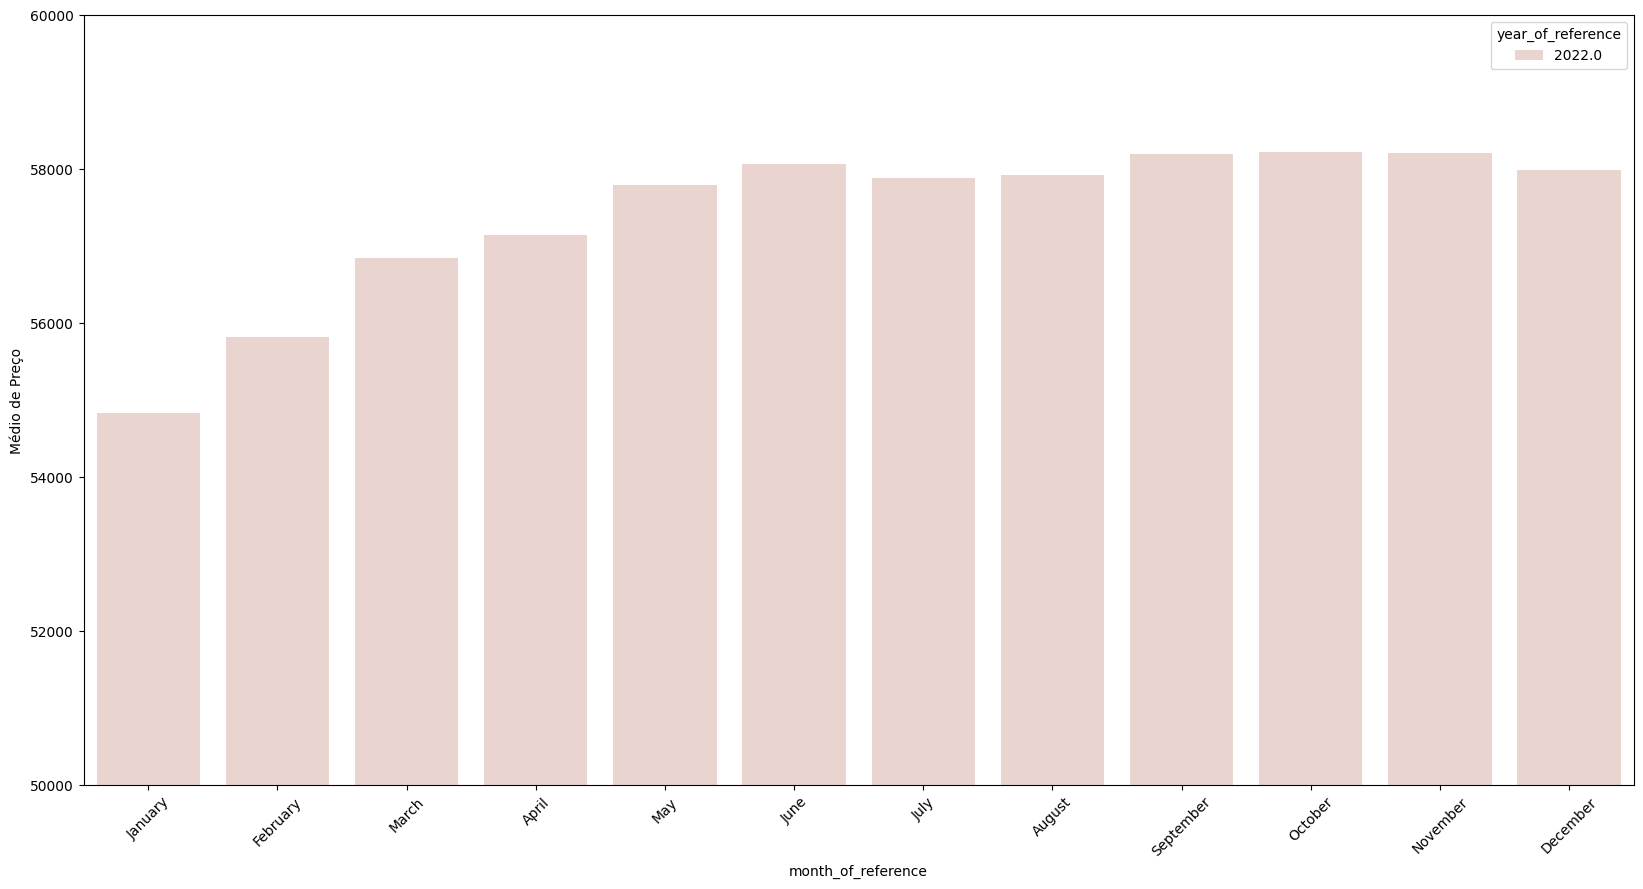
\includegraphics[width=1\linewidth]{apendices/fig/2_IAA002_3.png}
\caption*{Fonte: O autor (2024).}
\end{figure}



\begin{adjustwidth}{1em}{}
\textbf{d. Gere um gráfico da distribuição da média de preço dos carros por marca e tipo de engrenagem}
\end{adjustwidth}
\begin{lstlisting}[language=Python, style=input]
print(dados["gear"].unique()) # verificar os valores da coluna gear
\end{lstlisting}
\begin{lstlisting}[language=, style=output]
['manual' 'automatic']
\end{lstlisting}
\begin{lstlisting}[language=Python, style=input]
plt.figure(figsize=(20,10))
sns.barplot(x='brand', y='avg_price_brl', hue='gear', data=dados, hue_order=['manual', 'automatic'])
\end{lstlisting}
\begin{figure}[H]
\centering
\caption{Distribuição da média de preço dos carros por marca e tipo de engrenagem}
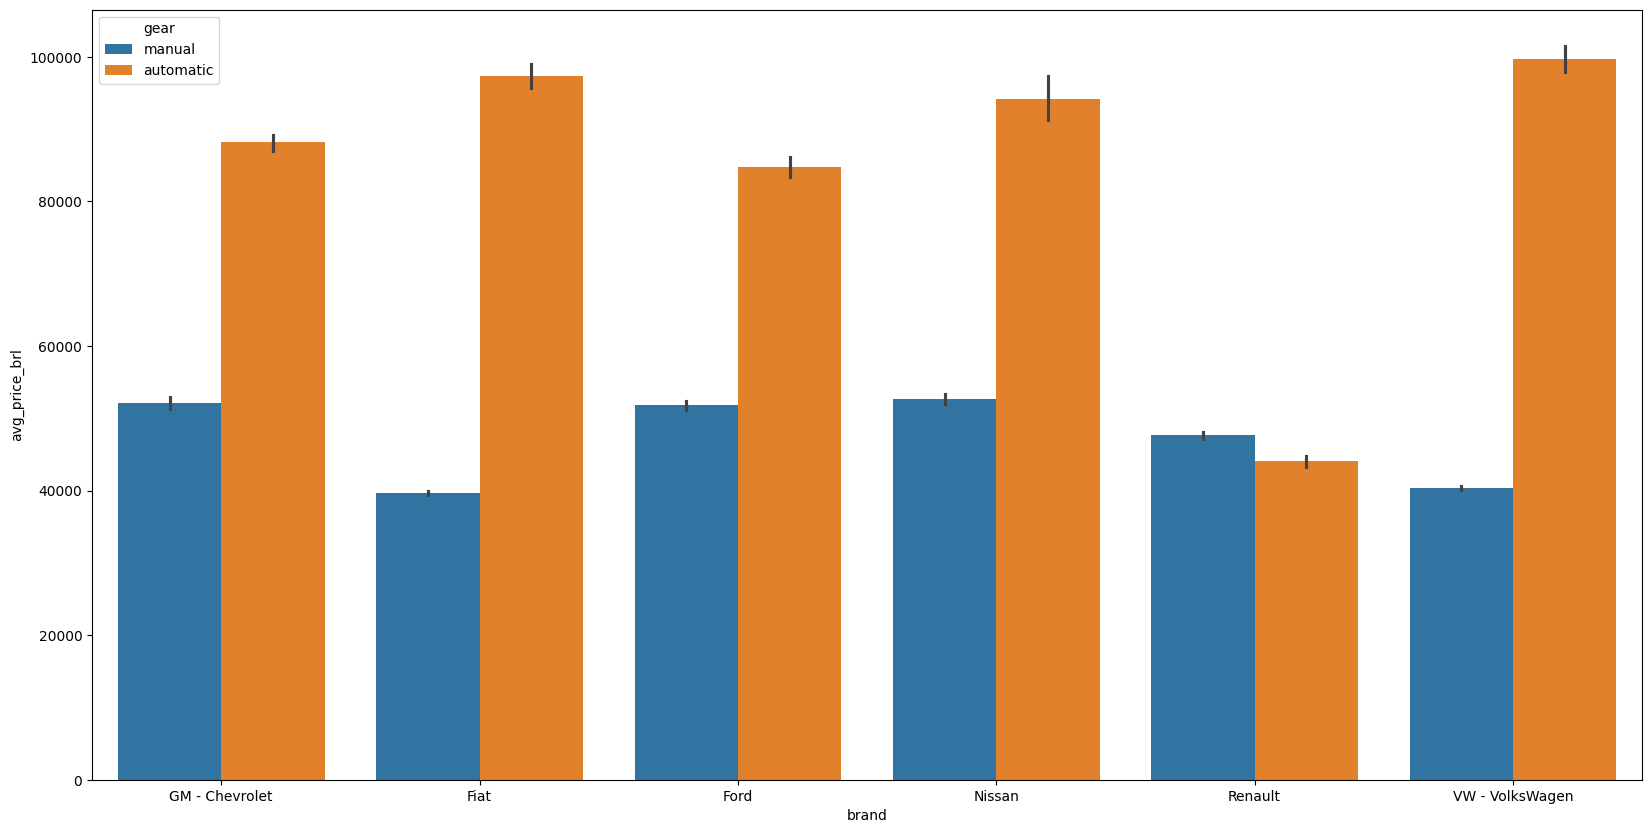
\includegraphics[width=1\linewidth]{apendices/fig/2_IAA002_4.png}
\caption*{Fonte: O autor (2024).}
\end{figure}

\begin{adjustwidth}{1em}{}
\textbf{e. Dê uma breve explicação (máximo de quatro linhas) sobre os resultados gerados no item d}
\end{adjustwidth}

O preço médio de carros com engrenagem (marcha) automática é superior aos com engrenagem manual em 5 das 6 marcas. Somente a Renault tem preços médios com ligeira superioridade nos carros com engrenagem manual. Nas marcas Fiat e Volkswagem os carro com engrenagem automática tem preço médio maiores do que o dobro dos carros com engrenagem manual.

\begin{adjustwidth}{1em}{}
\textbf{f. Gere um gráfico da distribuição da média de preço dos carros por marca e tipo de combustível}
\end{adjustwidth}
\begin{lstlisting}[language=Python, style=input]
print(dados["fuel"].unique()) # verificar os valores da coluna fuel
\end{lstlisting}
\begin{lstlisting}[language=, style=output]
['Gasoline' 'Alcohol' 'Diesel']
\end{lstlisting}
\begin{lstlisting}[language=Python, style=input]
plt.figure(figsize=(20,10))
sns.barplot(x='brand', y='avg_price_brl', hue='fuel', data=dados, hue_order=['Diesel', 'Gasoline', 'Alcohol'])
\end{lstlisting}
\begin{figure}[H]
\centering
\caption{Distribuição da média de preço dos carros por marca e tipo de combustível}
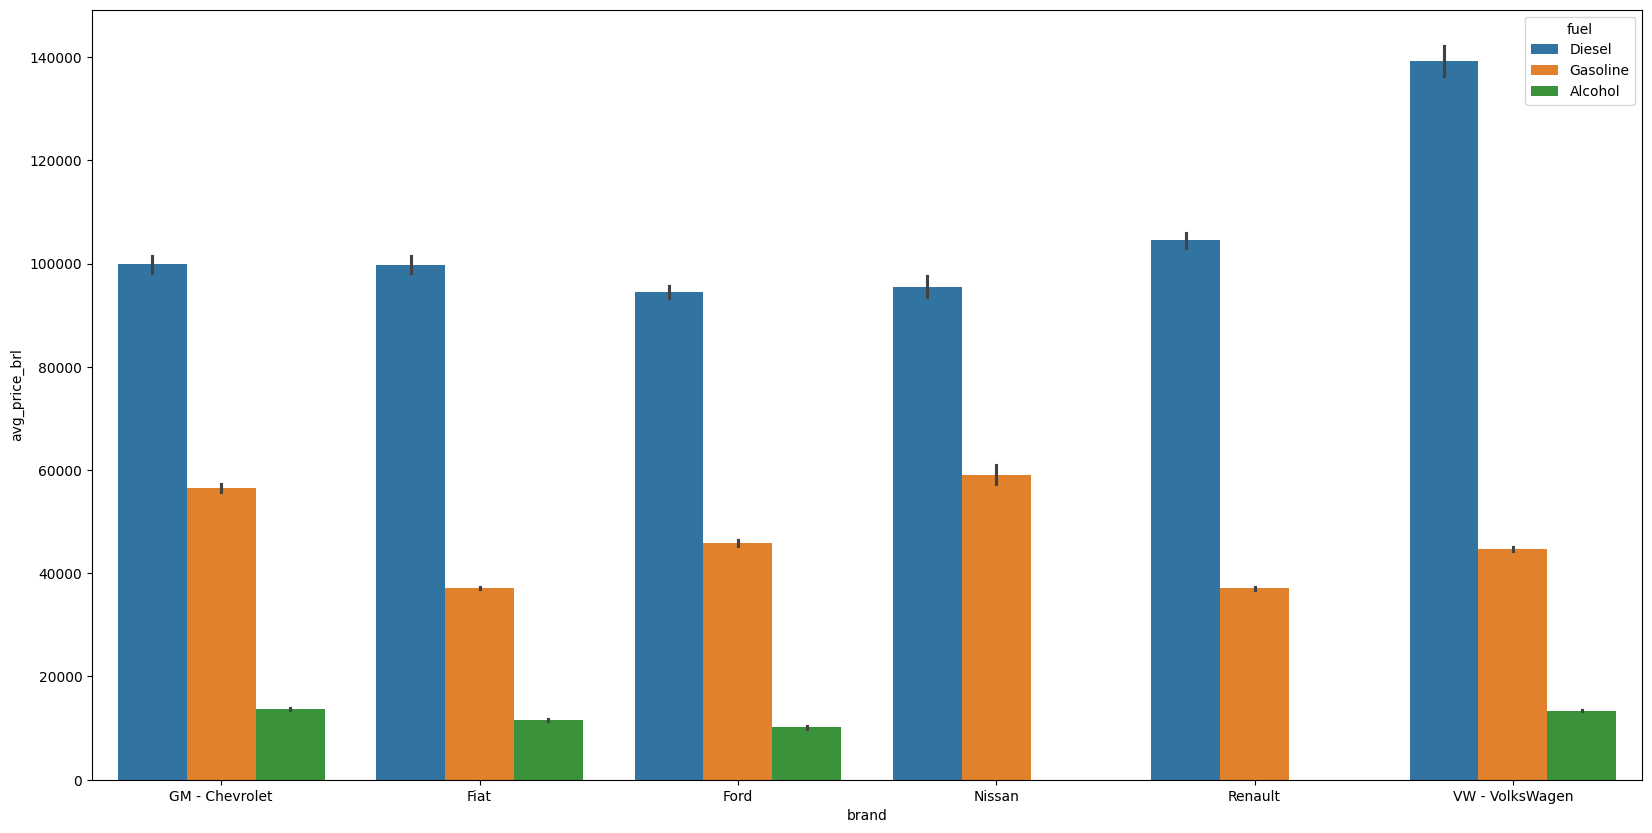
\includegraphics[width=1\linewidth]{apendices/fig/2_IAA002_5.png}
\caption*{Fonte: O autor (2024).}
\end{figure}

\begin{adjustwidth}{1em}{}
\textbf{g. Dê uma breve explicação (máximo de quatro linhas) sobre os resultados gerados no item f}
\end{adjustwidth}

Carros com o combustível Diesel tem os maiores preços médios em todas as marcas. O que faz sentido haja visto que motores a Diesel são comumente encontrados em carros maiores e de maiores valores. Veículos a Gasolina são os segundos com maiores preços médios em todas as marcas. Vale salientar que, nesta base, os veículos Flex (que podem consumir álcool e gasolina) estão categorizados como Gasolina.  Veículos a Álcool tem os menores preços médios nas marcas GM, Fiat, Ford e VM. As marcas Nissan e Renault não apresentaram veículos com combustível álcool.


\subsection*{\textbf{3 Aplicação de modelos de machine learning para prever o preço médio dos carros}}

\begin{adjustwidth}{1em}{}
\textbf{a. Escolha as variáveis \textbf{numéricas} (modelos de Regressão) para serem as variáveis independentes do modelo. A
variável target é \textbf{avg\_price. Observação:} caso julgue necessário, faça a transformação de variáveis
categóricas em variáveis numéricas para inputar no modelo. Indique \textbf{quais variáveis} foram transformadas e
\textbf{como} foram transformadas}
\end{adjustwidth}

\begin{lstlisting}[language=Python, style=input]
sns.boxplot(dados['avg_price_brl']).set_title("Distribuição dos preços dos carros") 
\end{lstlisting}
\begin{figure}[H]
\centering
\caption{Distribuição dos preços dos carros}
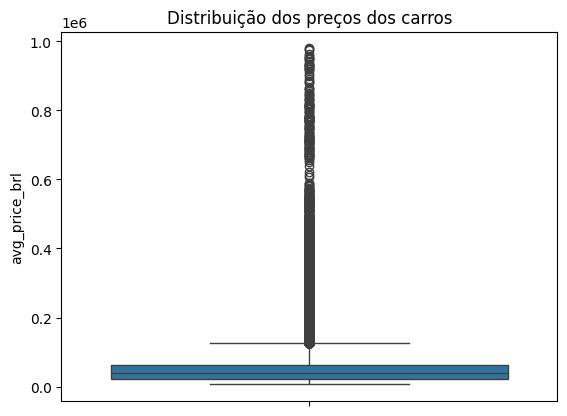
\includegraphics[width=.8\linewidth]{apendices/fig/2_IAA002_6.png}
\caption*{Fonte: O autor (2024).}
\end{figure}
\begin{lstlisting}[language=Python, style=input]
# Transformação da coluna modelo (model) de categórica para numérica
dados['model'] = LabelEncoder().fit_transform(dados['model']) 

# Transformação da coluna engrenagem (gear) de categórica para numérica
dados['gear'] = LabelEncoder().fit_transform(dados['gear']) 
dados.head()

# Transformação da coluna combustível (fuel) de categórica para numérica
dados['fuel'] = LabelEncoder().fit_transform(dados['fuel']) 
dados.head()
\end{lstlisting}
\begin{table}[H]
\centering
\begin{tcolorbox}[myoutputstyle, width=1.1\textwidth, enlarge left by=-1cm]
%\resizebox{\textwidth}{!}{ % scales table to fit page width
\renewcommand{\arraystretch}{1.2} % more vertical space in rows
\setlength{\tabcolsep}{6pt} % adjust horizontal padding between columns
\resizebox{0.95\textwidth}{!}{
\begin{tabular}{rrrrllllllll}
\hline
\textbf{ID} & \textbf{Year} & \textbf{Month} & \textbf{FIPE Code} & \textbf{Auth} & \textbf{Brand} & \textbf{Model} & \textbf{Fuel} & \textbf{Gear} & \textbf{Engine} & \textbf{Year Model} & \textbf{Avg. Price (BRL)} \\
\hline
0 & 2021.0 & January & 004001-0 & cfzlctzfwrcp & GM - Chevrolet & 297 & 2 & 1 & 1 & 2002.0 & 9162.0 \\
1 & 2021.0 & January & 004001-0 & cdqwxwpw3y2p & GM - Chevrolet & 297 & 2 & 1 & 1 & 2001.0 & 8832.0 \\
2 & 2021.0 & January & 004001-0 & cb1t3xwwj1xp & GM - Chevrolet & 297 & 2 & 1 & 1 & 2000.0 & 8388.0 \\
3 & 2021.0 & January & 004001-0 & cb9gct6j65r0 & GM - Chevrolet & 297 & 0 & 1 & 1 & 2000.0 & 8453.0 \\
4 & 2021.0 & January & 004003-7 & g15wg0gbz1fx & GM - Chevrolet & 260 & 2 & 1 & 1,6 & 2001.0 & 12525.0 \\
\hline
\end{tabular}
}
\end{tcolorbox}
%\caption{Vehicle data with numeric codes for fuel and gear types}
%\label{tab:vehicle_data_encoded}
\end{table}
\begin{lstlisting}[language=Python, style=input]
# Variável dados_num contém apenas variáveis numéricas de interesse (exclui o restante)
dados_num = dados.drop(['year_of_reference', 'month_of_reference', 'fipe_code', 'authentication', 'brand', 'engine_size'],axis = 1)

sns.heatmap(dados_num.corr("spearman"), annot = True)
plt.title("Mapa de Correlação das Variáveis Numéricas\n", fontsize = 15)
plt.show()
\end{lstlisting}
\begin{figure}[H]
\centering
\caption{Mapa de Correlação das Variáveis Numéricas}
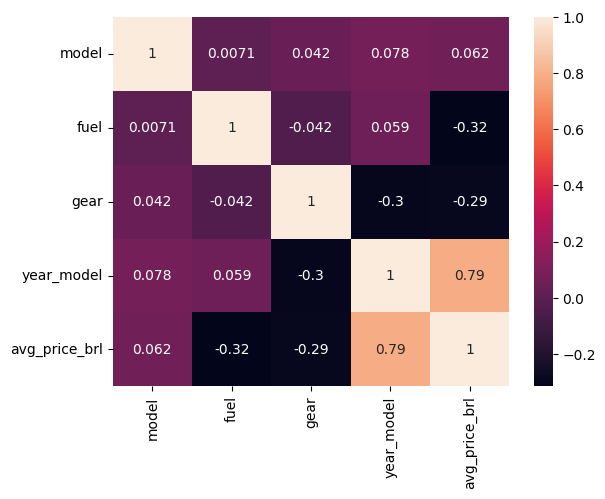
\includegraphics[width=.8\linewidth]{apendices/fig/2_IAA002_7.png}
\caption*{Fonte: O autor (2024).}
\end{figure}
\begin{lstlisting}[language=Python, style=input]
# Variável X contém apenas variáveis numéricas de interesse para a análise, excluindo a variável target 
X = dados_num.drop(['avg_price_brl'],axis = 1)

Y = dados_num['avg_price_brl']
\end{lstlisting}


\begin{adjustwidth}{1em}{}
\textbf{b. Crie partições contendo 75\% dos dados para treino e 25\% para teste}
\end{adjustwidth}
\begin{lstlisting}[language=Python, style=input]
# Divisão: 30% dos dados são de teste e 70% de treinamento
X_train, X_test, Y_train, Y_test = train_test_split(X, Y, test_size = 0.25, random_state = 42)
\end{lstlisting}

\begin{adjustwidth}{1em}{}
\textbf{c. Treine modelos RandomForest (biblioteca RandomForestRegressor) e XGBoost (biblioteca XGBRegressor) para predição
dos preços dos carros. \textbf{Observação}: caso julgue necessário, mude os parâmetros dos modelos e rode novos
modelos. Indique quais parâmetros foram inputados e indique o treinamento de cada modelo}
\end{adjustwidth}
\begin{lstlisting}[language=Python, style=input]
#RandomForest
model_rf = RandomForestRegressor()
model_rf.fit(X_train, Y_train)
\end{lstlisting}

\begin{lstlisting}[language=Python, style=input]
#RandomForest com parâmetros
n_estimators = [5,20,50,100] # number of trees in the random forest
max_features = ['auto', 'sqrt'] # number of features in consideration at every split
max_depth = [int(x) for x in np.linspace(10, 120, num = 12)] # maximum number of levels allowed in each decision tree
min_samples_split = [2, 6, 10] # minimum sample number to split a node
min_samples_leaf = [1, 3, 4] # minimum sample number that can be stored in a leaf node
bootstrap = [True, False] # method used to sample data points

random_grid = {'n_estimators': n_estimators, 'max_features': max_features, 'max_depth': max_depth, 'min_samples_split': min_samples_split, 
               'min_samples_leaf': min_samples_leaf, 'bootstrap': bootstrap}

rf = RandomForestRegressor()
rf_random = RandomizedSearchCV(estimator = rf,param_distributions = random_grid,
               n_iter = 100, cv = 5, verbose=2, random_state=35, n_jobs = -1)

rf_random.fit(X_train, Y_train)

# Utilizando os melhores parâmetros encontrados
model_rf_parametros = RandomForestRegressor(max_depth=70, min_samples_leaf=1, min_samples_split=2, n_estimators=20, random_state=80)

model_rf_parametros.fit(X_train, Y_train)
\end{lstlisting}

\begin{lstlisting}[language=Python, style=input]
#XGBoost
model_xgboost = XGBRegressor()
model_xgboost.fit(X_train, Y_train)
\end{lstlisting}


\begin{adjustwidth}{1em}{}
\textbf{d. Grave os valores preditos em variáveis criadas}
\end{adjustwidth}
\begin{lstlisting}[language=Python, style=input]
#RandomForest
valores_preditos_rf = model_rf.predict(X_test)
valores_preditos_rf 
\end{lstlisting}

\begin{lstlisting}[language=Python, style=input]
#RandomForest com parâmetros
valores_preditos_rf_parametros = model_rf_parametros.predict(X_test)
valores_preditos_rf_parametros
\end{lstlisting}

\begin{lstlisting}[language=Python, style=input]
#XGBoost
valores_preditos_xgboost = model_xgboost.predict(X_test)
valores_preditos_xgboost
\end{lstlisting}

\begin{adjustwidth}{1em}{}
\textbf{e. Realize a análise de importância das variáveis para estimar a variável target, \textbf{para cada modelo treinado}}
\end{adjustwidth}
\begin{lstlisting}[language=Python, style=input]
#RandomForest
model_rf.feature_importances_
feature_importances_rf = pd.DataFrame(model_rf.feature_importances_, index = X_train.columns, columns=['importance']).sort_values('importance', ascending = False)
feature_importances_rf 
\end{lstlisting}
\begin{table}[H]
\centering
\begin{tcolorbox}[myoutputstyle]
\begin{tabular}{lr}
\hline
\textbf{Feature} & \textbf{Importance} \\
\hline
model      & 0.439964 \\
year\_model & 0.358480 \\
fuel       & 0.179241 \\
gear       & 0.022315 \\
\hline
\end{tabular}
\end{tcolorbox}
%\caption{Feature importance values}
%\label{tab:feature_importance}
\end{table}


\begin{lstlisting}[language=Python, style=input]
#RandomForest com parâmetros
model_rf_parametros.feature_importances_
feature_importances_rf_param = pd.DataFrame(model_rf_parametros.feature_importances_, index = X_train.columns, columns=['importance']).sort_values('importance', ascending = False)
feature_importances_rf_param
\end{lstlisting}
\begin{table}[H]
\centering
\begin{tcolorbox}[myoutputstyle]
\begin{tabular}{lr}
\hline
\textbf{Feature} & \textbf{Importance} \\
\hline
model       & 0.442857 \\
year\_model & 0.356757 \\
fuel        & 0.178231 \\
gear        & 0.022155 \\
\hline
\end{tabular}
\end{tcolorbox}
%\caption{Updated feature importance values}
%\label{tab:updated_feature_importance}
\end{table}


\begin{lstlisting}[language=Python, style=input]
#XGBoost
model_xgboost.feature_importances_
feature_importances_x = pd.DataFrame(model_xgboost.feature_importances_, index = X_train.columns, columns=['importance']).sort_values('importance', ascending = False)
feature_importances_x
\end{lstlisting}
\begin{table}[H]
\centering
\begin{tcolorbox}[myoutputstyle]
\begin{tabular}{lr}
\hline
\textbf{Feature} & \textbf{Importance} \\
\hline
fuel        & 0.699523 \\
year\_model & 0.160642 \\
model       & 0.088919 \\
gear        & 0.050917 \\
\hline
\end{tabular}
\end{tcolorbox}
%\caption{Feature importance values (latest version)}
%\label{tab:feature_importance_latest}
\end{table}



\begin{adjustwidth}{1em}{}
\textbf{f. Dê uma breve explicação (máximo de quatro linhas) sobre os resultados encontrados na análise de importância de
variáveis}
\end{adjustwidth}

Tanto no modelo Random Forest, quando no modelo Random Forest com parâmetros, as variáveis mais importantes foram modelo e ano do modelo (model e year\_model) com quse 80\% de importância. Somando a combustível (fuel) chegamos a 97\% de importância. Tornando quase irrelevante a variável engrenagem (gear). Para o modelo XGBoost temos como variável mais importante o combustível (fuel) com aproximadamente 70\% e seguido de ano do modelo com 16\%. Modelo e engrenagem (model e gear) aparecem com menos de 10\% cada.

\begin{adjustwidth}{1em}{}
\textbf{g. Escolha o melhor modelo com base nas métricas de avaliação MSE, MAE e R²}
\end{adjustwidth}
\begin{lstlisting}[language=Python, style=input]
#RandomForest
mse_rf = mean_squared_error(Y_test, valores_preditos_rf)
mae_rf = mean_absolute_error(Y_test, valores_preditos_rf)
r2_rf = r2_score(Y_test, valores_preditos_rf)
mse_rf
mae_rf
r2_rf
\end{lstlisting}
\begin{lstlisting}[language=, style=output]
54633997.34991135
4215.705784378993
0.97969945241549
\end{lstlisting}


\begin{lstlisting}[language=Python, style=input]
#RandomForest com parâmetros
mse_rf_param = mean_squared_error(Y_test, valores_preditos_rf_parametros)
mae_rf_param = mean_absolute_error(Y_test, valores_preditos_rf_parametros)
r2_rf_param = r2_score(Y_test, valores_preditos_rf_parametros)
mse_rf_param
mae_rf_param
r2_rf_param
\end{lstlisting}
\begin{lstlisting}[language=, style=output]
54716253.201698475
4216.618281471371
0.9796688883177797
\end{lstlisting}


\begin{lstlisting}[language=Python, style=input]
#XGBoost
mse_x = mean_squared_error(Y_test, valores_preditos_xgboost)
mae_x = mean_absolute_error(Y_test, valores_preditos_xgboost)
r2_x = r2_score(Y_test, valores_preditos_xgboost)
mse_x
mae_x
r2_x
\end{lstlisting}
\begin{lstlisting}[language=, style=output]
297039446.66991967
6429.30300193814
0.8896280024509496
\end{lstlisting}

\begin{adjustwidth}{1em}{}
\textbf{h. Dê uma breve explicação (máximo de quatro linhas) sobre qual modelo gerou o melhor resultado e a métrica de
avaliação utilizada}
\end{adjustwidth}

Levando em conta a acurácia resultante da métrica R2, temos os seguintes resultados:
\begin{itemize}
    \item Random Forest: 98\%
    \item Random Forest com parâmetros: 98\%
    \item XGBoost: 89\%
\end{itemize}
Desta forma, temos um empate entre Random Forest e Random Forest com parâmetros. Para fins de entendimento, trazemos a comparação dos resultados de MSE e MAE (quanto menores, melhores os resultados):

\begin{itemize}
    \item MSE
    \begin{itemize}
        \item Random Forest: 54.622.503
        \item Random Forest com parâmetros: 54.716.253
    \end{itemize}
    \item MAE
    \begin{itemize}
        \item Random Forest: 4215
        \item Random Forest com parâmetros: 4217
    \end{itemize}
\end{itemize}

Como podemos ver, há uma ligeira vantagem no uso do Random Forest, sem parâmetros. Assim sendo, concluímos que o melhor resultado preditivo foi obtido através do modelo Random Forest.
\label{ap:ap03}
\chapter{Linguagem R}
\section*{\textbf{A - ENUNCIADO}}
\subsection{Pesquisa com Dados de Satélite (Satellite)}



O banco de dados consiste nos valores multiespectrais de pixels em vizinhanças 3x3 em uma imagem de satélite, e na
classificação associada ao pixel central em cada vizinhança. O objetivo é prever esta classificação, dados os valores
multiespectrais.

Um quadro de imagens do Satélite Landsat com MSS (\textit{Multispectral Scanner System}) consiste em quatro imagens
digitais da mesma cena em diferentes bandas espectrais. Duas delas estão na região visível (correspondendo
aproximadamente às regiões verde e vermelha do espectro visível) e duas no infravermelho (próximo). Cada pixel é uma
palavra binária de 8 bits, com 0 correspondendo a preto e 255 a branco. A resolução espacial de um pixel é de cerca de
80m x 80m. Cada imagem contém 2340 x 3380 desses pixels. O banco de dados é uma subárea (minúscula) de uma cena,
consistindo de 82 x 100 pixels. Cada linha de dados corresponde a uma vizinhança quadrada de pixels 3x3 completamente
contida dentro da subárea 82x100. Cada linha contém os valores de pixel nas quatro bandas espectrais (convertidas em
ASCII) de cada um dos 9 pixels na vizinhança de 3x3 e um número indicando o rótulo de classificação do pixel central.

As classes são: solo vermelho, colheita de algodão, solo cinza, solo cinza úmido, restolho de vegetação, solo cinza
muito úmido.

Os dados estão em ordem aleatória e certas linhas de dados foram removidas, portanto você não pode reconstruir a imagem
original desse conjunto de dados. Em cada linha de dados, os quatro valores espectrais para o pixel superior esquerdo
são dados primeiro, seguidos pelos quatro valores espectrais para o pixel superior central e, em seguida, para o pixel
superior direito, e assim por diante, com os pixels lidos em sequência, da esquerda para a direita e de cima para
baixo. Assim, os quatro valores espectrais para o pixel central são dados pelos atributos 17, 18, 19 e 20. Se você
quiser, pode usar apenas esses quatro atributos, ignorando os outros. Isso evita o problema que surge quando uma
vizinhança 3x3 atravessa um limite.

O banco de dados se encontra no pacote \textbf{mlbench} e é completo (não possui dados faltantes).
\newpage
Tarefas:

\begin{enumerate}[series=listWWNumxxii,label=\arabic*.,ref=\arabic*]
\item Carregue a base de dados Satellite
\item Crie partições contendo 80\% para treino e 20\% para teste
\item Treine modelos RandomForest, SVM e RNA para predição destes dados. 
\item Escolha o melhor modelo com base em suas matrizes de confusão. 
\item Indique qual modelo dá o melhor o resultado e a métrica utilizada
\end{enumerate}




\subsection{Estimativa de Volumes de Árvores}



\textcolor{black}{Modelos de aprendizado de máquina são bastante usados na área da engenharia florestal (mensuração
florestal) para, por exemplo, estimar o volume de madeira de árvores sem ser necessário abatê-las.}

\textcolor{black}{O processo é feito pela coleta de dados (dados observados) através do abate de algumas árvores, onde
sua altura, diâmetro na altura do peito (dap), etc, são medidos de forma exata. Com estes dados, treina-se um modelo de
AM que pode estimar o volume de outras árvores da população.}

\textcolor{black}{Os modelos, chamados alométricos, são usados na área há muitos anos e são baseados em regressão
(linear ou não) para encontrar uma equação que descreve os dados. Por exemplo, o modelo de Spurr é dado por:}



{\centering
\textbf{\textcolor{black}{Volume = b0 + b1 *
dap}}\textbf{\textcolor{black}{\textsuperscript{2}}}\textbf{\textcolor{black}{ * Ht}}
\par}



\textcolor{black}{Onde dap é o diâmetro na altura do peito (1,3metros), Ht é a altura total. Tem-se vários modelos
alométricos, cada um com uma determinada característica, parâmetros, etc. Um modelo de regressão envolve aplicar os
dados observados e encontrar b0 e b1 no modelo apresentado, gerando assim uma equação que pode ser usada para prever o
volume de outras árvores.}

\textcolor{black}{Dado o arquivo }\textbf{\textcolor{black}{Volumes.csv}}\textcolor{black}{, que contém os dados de
observação, escolha um modelo de aprendizado de máquina com a melhor estimativa, a partir da estatística de
correlação.}



\textcolor{black}{Tarefas}

\begin{enumerate}[series=listWWNumxx,label=\arabic*.,ref=\arabic*]
\item \textcolor{black}{Carregar o arquivo Volumes.csv (http://www.razer.net.br/datasets/Volumes.csv)}
\item \textcolor{black}{Eliminar a coluna NR, que só apresenta um número sequencial}
\item \textcolor{black}{Criar partição de dados: treinamento 80\%, teste 20\%}
\item \textcolor{black}{Usando o pacote {\textquotedbl}caret{\textquotedbl}, treinar os modelos: Random Forest (rf), SVM
(svmRadial), Redes Neurais (neuralnet) e o modelo alométrico de SPURR}
\end{enumerate}

\begin{itemize}
\item \textcolor{black}{O modelo alométrico é dado por: Volume = b0 + b1 *
dap}\textcolor{black}{\textsuperscript{2}}\textcolor{black}{ * Ht}
\end{itemize}


\foreignlanguage{english}{\textbf{\textcolor{black}{alom {\textless}- nls(VOL \textasciitilde{} b0 + b1*DAP*DAP*HT, dados,
start=list(b0=0.5, b1=0.5)}}}\foreignlanguage{english}{\textcolor{black}{)}}



\begin{enumerate}[resume*=listWWNumxx,start=5]
\item \textcolor{black}{Efetue as predições nos dados de teste}
\item \textcolor{black}{Crie suas próprias funções (UDF) e calcule as seguintes métricas entre a predição e os dados
observados}
\end{enumerate}


\textbf{Coeficiente de determinação: }$R^2$

\begin{center}
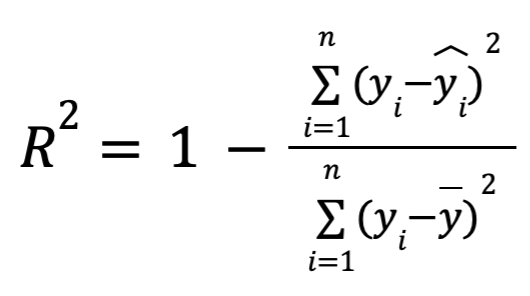
\includegraphics[width=5.191cm,height=2.9cm]{apendices/fig/IAA003_1.png} 
\end{center}

\textcolor{black}{onde } $y_i$ \textcolor{black}{\ é o valor observado, } $\widehat {y_i}$ \textcolor{black}{\ é o valor
predito e } $\overline y$ \textcolor{black}{\ é a média dos valores } $y_i$ \textcolor{black}{\ observados. Quanto mais
perto de 1 melhor é o modelo;}



\begin{itemize}
\item \textcolor{black}{Erro padrão da estimativa: S}\textcolor{black}{\textsubscript{yx}}
\end{itemize}

\begin{center}
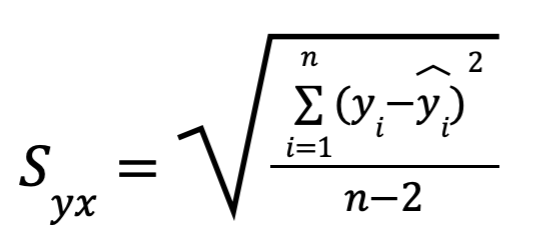
\includegraphics[width=5.117cm,height=2.32cm]{apendices/fig/IAA003_2.png} 
\end{center}

\textcolor{black}{esta métrica indica erro, portanto quanto mais perto de 0 melhor é o modelo;}



\begin{itemize}
\item \textcolor{black}{Syx\%}
\end{itemize}
\begin{center}
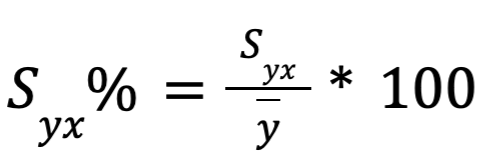
\includegraphics[width=3.688cm,height=1.235cm]{apendices/fig/IAA003_3.png}
\end{center}


\textcolor{black}{esta métrica indica porcentagem de erro, portanto quanto mais perto de 0 melhor é o modelo;}



\begin{enumerate}[resume*=listWWNumxx,start=7]
\item \textcolor{black}{Escolha o melhor modelo.}
\end{enumerate}

%%%%%%%%%%%%%%%%%%%%%%%%%%%%%%%%%%%%%%%%%%%%%%%%%%%%%%%%%%%%%%%%%%%%%%%%%%%%%%%%%%%%%%%%%%%%%
\section*{\textbf{B - RESOLUÇÃO}}
\lipsum[30]
\label{ap:ap04}
\chapter{Estatística Aplicada I}
\section*{\textbf{A - ENUNCIADO}}
\begin{enumerate}[series=listWWNumxxvi,label=\arabic*),ref=\arabic*]
\item \textbf{Gráficos e tabelas}
\end{enumerate}

\bigskip

(15 pontos) Elaborar os gráficos box-plot e histograma das variáveis “age” (idade da esposa) e “husage” (idade do
marido) e comparar os resultados

(15 pontos) Elaborar a tabela de frequencias das variáveis “age” (idade da esposa) e “husage” (idade do marido) e
comparar os resultados


\bigskip

\begin{enumerate}[resume*=listWWNumxxvi]
\item \textbf{Medidas de posição e dispersão}
\end{enumerate}

\bigskip

(15 pontos) Calcular a média, mediana e moda das variáveis “age” (idade da esposa) e “husage” (idade do marido) e
comparar os resultados

(15 pontos) Calcular a variância, \ desvio padrão e coeficiente de variação das variáveis “age” (idade da esposa) e
“husage” (idade do marido) e comparar os resultados


\bigskip

\begin{enumerate}[resume*=listWWNumxxvi]
\item \textbf{Testes paramétricos ou não paramétricos}
\end{enumerate}

\bigskip

(40 pontos) Testar se as médias (se você escolher o teste paramétrico) \ ou as medianas (se você escolher o teste não
paramétrico) das variáveis “age” (idade da esposa) e “husage” (idade do marido) são iguais, construir os intervalos de
confiança e comparar os resultados.

Obs: 

Você deve fazer os testes necessários (e mostra-los no documento pdf) para saber se você deve usar o unpaired test
(paramétrico) ou o teste U de Mann-Whitney (não paramétrico), justifique sua resposta sobre a escolha.

Lembre-se de que os intervalos de confiança já são mostrados nos resultados dos testes citados no item 1 acima. 


%%%%%%%%%%%%%%%%%%%%%%%%%%%%%%%%%%%%%%%%%%%%%%%%%%%%%%%%%%%%%%%%%%%%%%%%%%%%%%%%%%%%%%%%%%%%%
\section*{\textbf{B - RESOLUÇÃO}}
\lipsum[30]
\label{ap:ap05}
\chapter{Estatística Aplicada II}
\section*{\textbf{A - ENUNCIADO}}

\subsection*{\textbf{1 Regressões Ridge, Lasso e ElasticNet}}


\begin{enumerate}[label=\alph*)]
\item \textbf{(100 pontos) }Fazer as regressões Ridge, Lasso e ElasticNet com a variável dependente “lwage” (salário-hora da
esposa em logaritmo neperiano) e todas as demais variáveis da base de dados são variáveis explicativas (todas essas
variáveis tentam explicar o salário-hora da esposa). No pdf você deve colocar a rotina utilizada, mostrar em uma tabela
as estatísticas dos modelos (RMSE e R\textsuperscript{2}) e concluir qual o melhor modelo entre os três, e mostrar o
resultado da predição com intervalos de confiança para os seguintes valores:

husage = 40 \ \ \ \ \ \ \ \ \ (anos – idade do marido)

husunion = 0 \ \ \ \ \ \ \ (marido não possui união estável)

husearns = 600 \ \ \ (US\$ renda do marido por semana)

huseduc = 13 \ \ \ \ \ \ (anos de estudo do marido)

husblck = 1 \ \ \ \ \ \ \ \ \ \ (o marido é preto)

hushisp = 0 \ \ \ \ \ \ \ \ \ \ (o marido não é hispânico)

hushrs = 40 \ \ \ \ \ \ \ \ \ \ (horas semanais de trabalho do marido)

kidge6 = 1 \ \ \ \ \ \ \ \ \ \ \ \ (possui filhos maiores de 6 anos)

age = 38 \ \ \ \ \ \ \ \ \ \ \ \ \ \ \ (anos – idade da esposa)

black = 0 \ \ \ \ \ \ \ \ \ \ \ \ \ \ (a esposa não é preta)

educ = 13 \ \ \ \ \ \ \ \ \ \ \ \ \ (anos de estudo da esposa)

hispanic = 1 \ \ \ \ \ \ \ \ \ (a esposa é hispânica)

union = 0 \ \ \ \ \ \ \ \ \ \ \ \ \ (esposa não possui união estável)

exper = 18 \ \ \ \ \ \ \ \ \ \ \ (anos de experiência de trabalho da esposa)

kidlt6 = 1 \ \ \ \ \ \ \ \ \ \ \ \ \ (possui filhos menores de 6 anos)
\end{enumerate}
obs: lembre-se de que a variável dependente “lwage” já está em logarítmo, portanto voçê não precisa aplicar o logaritmo
nela para fazer as regressões, mas é necessário aplicar o antilog para obter o resultado da predição. 


%%%%%%%%%%%%%%%%%%%%%%%%%%%%%%%%%%%%%%%%%%%%%%%%%%%%%%%%%%%%%%%%%%%%%%%%%%%%%%%%%%%%%%%%%%%%%
\section*{\textbf{B - RESOLUÇÃO}}
\begin{adjustwidth}{1em}{}
\textbf{a) Fazer as regressões Ridge, Lasso e ElasticNet com a variável dependente “lwage” (salário-hora da
esposa em logaritmo neperiano) e todas as demais variáveis da base de dados são variáveis explicativas (todas essas
variáveis tentam explicar o salário-hora da esposa).}
\end{adjustwidth}

\subsection*{PADRONIZAÇÃO DOS DADOS}

\begin{lstlisting}[language=R, style=input]
cols = c('husage', 'husearns', 'huseduc', 'hushrs', 'earns', 'age', 'educ', 'exper', 'lwage')
pre_proc_val <- preProcess(train[,cols], method = c("center", "scale"))

train[,cols] = predict(pre_proc_val, train[,cols])
test[,cols] = predict(pre_proc_val, test[,cols])

cols_reg = c('husage', 'husunion', 'husearns', 'huseduc', 'husblck', 'hushisp', 'hushrs',
'kidge6', 'age', 'black', 'educ', 'hispanic', 'union', 'exper', 'kidlt6', 'lwage')

dummies <- dummyVars(lwage~husage+husunion+husearns+huseduc+husblck+
hushisp+hushrs+kidge6+age+black+educ+hispanic+union+exper+kidlt6, 
data = dat[,cols_reg])
train_dummies = predict(dummies, newdata = train[,cols_reg])
test_dummies = predict(dummies, newdata = test[,cols_reg])

x_train = as.matrix(train_dummies)
y_train = train$lwage

x_test = as.matrix(test_dummies)
y_test = test$lwage
\end{lstlisting}

\subsection*{REGRESSÃO RIDGE}
\begin{lstlisting}[language=R, style=input]
lambdas <- 10^seq(5, -5, by = -1)
ridge_lamb <- cv.glmnet(x_train, y_train, alpha = 0, lambda = lambdas, nfolds = 10)

best_lambda_ridge <- ridge_lamb$lambda.min
best_lambda_ridge

ridge_reg = glmnet(x_train, y_train, nlambda = 50, alpha = 0, family = 'gaussian', 
lambda = best_lambda_ridge)
ridge_reg

# Resultado
# (coeficientes)
ridge_reg[["beta"]]

predictions_train_ridge <- predict(ridge_reg, s = best_lambda_ridge, newx = x_train)
\end{lstlisting}

Visualizando o resultado da estimativa dos coeficientes percebemos que nem todas as variáveis explicam a variável dependente. Infelizmente as que explicam tem valor explicativo muito baixo, sendo somente as com certa relevância ``husearns'', ``husblck'', ``hushisp'', ``kidge6'', ``black'', ``educ'' e ``union''. \\

\begin{lstlisting}[language=R, style=output]
15 x 1 sparse Matrix of class "dgCMatrix"
                  s0
husage    0.02651324
husunion -0.04174920
husearns  0.23671354
huseduc   0.04804650
husblck   0.24319544
hushisp   0.11457810
hushrs   -0.07293064
kidge6   -0.16442536
age       0.04466390
black    -0.29066663
educ      0.30859463
hispanic -0.09979930
union     0.41614645
exper    -0.01411404
kidlt6   -0.02475760
\end{lstlisting}



\subsection*{REGRESSÃO LASSO}
\begin{lstlisting}[language=R, style=input]
lambdas <- 10^seq(5, -5, by = -.1)

lasso_lamb <- cv.glmnet(x_train, y_train, alpha = 1, lambda = lambdas, 
standardize = TRUE, nfolds = 10)

best_lambda_lasso <- lasso_lamb$lambda.min 
best_lambda_lasso

lasso_model <- glmnet(x_train, y_train, alpha = 1, lambda = best_lambda_lasso, 
standardize = TRUE)

lasso_model[["beta"]]

predictions_train_lasso <- predict(lasso_model, s = best_lambda_lasso, newx = x_train)
\end{lstlisting}

Visualizando o resultado da estimativa dos coeficientes percebemos que nem todas as variáveis explicam a variável dependente. Infelizmente as que explicam tem valor explicativo muito baixo, sendo somente as com certa relevância ``husearns'', ``husblck'', ``hushisp'', ``kidge6'', ``black'', ``educ'' e ``union''. Enquanto a variável ``exper'' teve tão pouco valor explicativo que foi a zero. \\

\begin{lstlisting}[language=R, style=output]
15 x 1 sparse Matrix of class "dgCMatrix"
                  s0
husage    0.02406805
husunion -0.04144957
husearns  0.23903324
huseduc   0.04539082
husblck   0.26797943
hushisp   0.11329929
hushrs   -0.07369940
kidge6   -0.16534640
age       0.03331493
black    -0.31556379
educ      0.31552507
hispanic -0.09716331
union     0.41807407
exper     .         
kidlt6   -0.02464497
\end{lstlisting}

\subsection*{REGRESSÃO ELASTICNET}
\begin{lstlisting}[language=R, style=input]
train_cont <- trainControl(method = "repeatedcv",
                           number = 10,
                           repeats = 5,
                           search = "random",
                           verboseIter = FALSE)

elastic_reg <- train(lwage~husage+husunion+husearns+huseduc+husblck+hushisp+
hushrs+kidge6+age+black+educ+hispanic+union+exper+kidlt6,
                     data = train,
                     method = "glmnet",
                     tuneLength = 20,
                     trControl = train_cont)

# O melhor parametro alpha escolhido eh:
#       alpha       lambda
#15     0.8015939   0.01293922
elastic_reg$bestTune

# E os parametros sao:
#elastic_reg[["finalModel"]][["beta"]]

predictions_train_elasticnet <- predict(elastic_reg, x_train)
\end{lstlisting}

\section*{COMPARANDO RESULTADOS}

\begin{lstlisting}[language=R, style=input]
eval_results <- function(true, predicted, df) {
  SSE <- sum((predicted - true)^2)
  SST <- sum((true - mean(true))^2)
  R_square <- 1 - SSE / SST
  RMSE = sqrt(SSE/nrow(df))
  
  # As metricas de performace do modelo:
  data.frame(
    RMSE = RMSE,
    Rsquare = R_square
  )
}

eval_with_params <- function(model, best_lambda = NULL) {
  husage = (40-pre_proc_val[["mean"]][["husage"]])/pre_proc_val[["std"]][["husage"]]
  husunion = 0
  husearns = (600-pre_proc_val[["mean"]][["husearns"]])/
  pre_proc_val[["std"]][["husearns"]]
  huseduc = (13-pre_proc_val[["mean"]][["huseduc"]])/pre_proc_val[["std"]][["huseduc"]]
  husblck = 1
  hushisp = 0
  hushrs = (40-pre_proc_val[["mean"]][["hushrs"]])/pre_proc_val[["std"]][["hushrs"]]
  kidge6 = 1
  age = (38-pre_proc_val[["mean"]][["age"]])/pre_proc_val[["std"]][["age"]]
  black = 0
  educ = (13-pre_proc_val[["mean"]][["educ"]])/pre_proc_val[["std"]][["educ"]]
  hispanic = 1
  union = 0
  exper = (18-pre_proc_val[["mean"]][["exper"]])/pre_proc_val[["std"]][["exper"]]
  kidlt6 = 1
  
  our_pred = as.matrix(data.frame(husage=husage, 
                                  husunion=husunion,
                                  husearns=husearns,
                                  huseduc=huseduc,
                                  husblck=husblck,
                                  hushisp=hushisp,
                                  hushrs=hushrs,
                                  kidge6=kidge6,
                                  age=age,
                                  black=black,
                                  educ=educ,
                                  hispanic=hispanic,
                                  union=union,
                                  exper=exper,
                                  kidlt6=kidlt6))
  
  prediction <- predict(model, s = best_lambda, newx = our_pred)
  
  if (is.null(best_lambda)) {
    prediction <- predict(model, our_pred)
  }
  
  wage_pred=(prediction*pre_proc_val[["std"]][["lwage"]])+
  pre_proc_val[["mean"]][["lwage"]]
  
  cat("Predicao: ", wage_pred, "\n")
  cat("Predicao exp: ", exp(wage_pred), "\n")
  
  return(wage_pred)
}

show_values <- function(wage_pred) {
  
  # O intervalo de confianca
  n <- nrow(train)
  m <- wage_pred
  s <- pre_proc_val[["std"]][["lwage"]]
  dam <- s/sqrt(n)
  CIlwr <- m + (qnorm(0.025))*dam # intervalo inferior
  CIupr <- m - (qnorm(0.025))*dam # intervalo superior
  
  cat("Intervalo inferior: ", CIlwr, "\n")
  cat("Intervalo superior: ", CIupr, "\n")
  
  cat("Intervalo inferior exp: ", exp(CIlwr), "\n")
  cat("Intervalo superior exp: ", exp(CIupr), "\n")
}

# -------- RIDGE -------- #

eval_results(y_train, predictions_train_ridge, train)

predictions_test <- predict(ridge_reg, s = best_lambda_ridge, newx = x_test)
eval_results(y_test, predictions_test, test)

predict_our_ridge <- eval_with_params(ridge_reg, best_lambda = best_lambda_ridge)

show_values(predict_our_ridge)

# -------- LASSO -------- #

eval_results(y_train, predictions_train_lasso, train)

predictions_test <- predict(lasso_model, s = best_lambda_lasso, newx = x_test)
eval_results(y_test, predictions_test, test)

predict_our_lasso <- eval_with_params(lasso_model, best_lambda = best_lambda_lasso)

show_values(predict_our_lasso)

# ------- ELATICNET ----- #

eval_results(y_train, predictions_train_elasticnet, train) 
predictions_test <- predict(elastic_reg, x_test)
eval_results(y_test, predictions_test, test)

predict_our_elastic <- eval_with_params(elastic_reg)

show_values(predict_our_elastic)
\end{lstlisting}

Observando a Tabela \ref{tab:metricas} abaixo observamos que os valores para as métricas de todos os modelos são muito próximas e também não muito boas, não descartando a hipótese de overfitting ou underfitting. Mesmo assim, a título de comparação observamos que o modelo Lasso se saiu ligeiraimente melhor do que os outros para o conjunto de dados de treinamento, enquanto o modelo Ridge se saiu ligeiramente melhor nos dados de teste.

\begin{table}[H]
\centering
\caption{Tabela de métricas dos modelos}
\begin{tabular}{c|c|c|c|c||}      
\cline{2-5}
    & \multicolumn{2}{c|}{Treinamento} & \multicolumn{2}{c||}{Teste}\\
\cline{2-5}
    & RMSE & Rsquare & RMSE & Rsquare\\
\cline{1-5}
\multicolumn{1}{||c|}{Ridge} & \cellcolor[HTML]{FFF8B8} 0.8485564 & \cellcolor[HTML]{FFF8B8} 0.2796022 & \cellcolor[HTML]{CAF2C2} 0.8488229 & \cellcolor[HTML]{CAF2C2} 0.3004756 \\
\cline{1-5}
\multicolumn{1}{||c|}{Lasso} & \cellcolor[HTML]{CAF2C2} 0.8485375 & \cellcolor[HTML]{CAF2C2} 0.2796343 & \cellcolor[HTML]{FFF8B8} 0.8488541 & \cellcolor[HTML]{FFF8B8} 0.3004242 \\
\cline{1-5}
\multicolumn{1}{||c|}{ElasticNet} & \cellcolor[HTML]{FFD6C9} 0.8495878 & \cellcolor[HTML]{FFD6C9} 0.2778498 & \cellcolor[HTML]{FFD6C9} 0.8490653 & \cellcolor[HTML]{FFD6C9} 0.3000762 \\                
\hline
\end{tabular}
\label{tab:metricas}
\end{table}

Na Tabela \ref{tab:predicao} pode-se observar os valores preditos pelos modelos para as váriaveis especificadas inicialmente.

\begin{table}[H]
\centering
\caption{Tabela de Predição e Intervalos de Confiança}
\begin{tabular}{c|c|c||}       
\cline{2-3}
           & \multicolumn{1}{c|}{Predição} & Intervalos de Confiança \\
\hline
\multicolumn{1}{||c|}{Ridge}      & 8.633904 & 8.442068 | 8.8301     \\
\hline
\multicolumn{1}{||c|}{Lasso}      & 8.746603 & 8.552263 | 8.945359     \\
\hline
\multicolumn{1}{||c|}{ElasticNet} & 8.160874 & 7.979548 | 8.34632    \\
\hline
\end{tabular}
\label{tab:predicao}
\end{table}
\label{ap:ap06}
\chapter{Arquitetura de dados}
\section*{\textbf{A - ENUNCIADO}}


\subsection*{\textbf{1 Construção de Características: Identificador automático de idioma}}

\textcolor{black}{O problema consiste em criar um modelo de reconhecimento de padrões que dado um texto de entrada, o
programa consegue classificar o texto e indicar a língua em que o texto foi escrito.}



\textcolor{black}{Parta do exemplo (notebook produzido no Colab) que foi disponibilidade e crie as funções para calcular
as diferentes características para o problema da identificação da língua do texto de entrada.}



\textcolor{black}{Nessa atividade é para {\textquotedbl}construir características{\textquotedbl}.}



\textcolor{black}{Meta: a acurácia deverá ser maior ou igual a 70\%.}



\textcolor{black}{Essa tarefa pode ser feita no Colab (Google) ou no Jupiter, em que deverá exportar o notebook e
imprimir o notebook para o formato PDF. Envie no UFPR Virtual os dois arquivos.}



\subsection*{\textbf{2 Melhore uma base de dados ruim}}



\textcolor{black}{Escolha uma base de dados pública para problemas de classificação, disponível ou com origem na UCI
Machine Learning.}



\textcolor{black}{Use o mínimo de intervenção para rodar a SVM e obtenha a matriz de confusão dessa base.}



\textcolor{black}{O trabalho começa aqui, escolha as diferentes tarefas discutidas ao longo da disciplina, para melhorar
essa base de dados, até que consiga efetivamente melhorar o resultado.}



\textcolor{black}{Considerando a acurácia para bases de dados balanceadas ou quase balanceadas, se o percentual da
acurácia original estiver em até 85\%, a meta será obter 5\%. Para bases com mais de 90\% de acurácia, a meta será
obter a melhora em pelo menos 2 pontos percentuais (92\% ou mais).}



\textcolor{black}{Nessa atividade deverá ser entregue o script aplicado (o notebook e o PDF correspondente).}



%%%%%%%%%%%%%%%%%%%%%%%%%%%%%%%%%%%%%%%%%%%%%%%%%%%%%%%%%%%%%%%%%%%%%%%%%%%%%%%%%%%%%%%%%%%%%
\section*{\textbf{B - RESOLUÇÃO}}
\begin{adjustwidth}{1em}{}
\textbf{1 Construção de Características: Identificador automático de idioma}
\end{adjustwidth}

\subsection*{\textbf{Identificador automático de idioma}}
\textbf{Problema:} Dados um texto de entrada, é possível identificar em qual língua o texto está escrito?

Entrada: ``texto qualquer''\\
\indent Saída: português ou inglês ou francês ou italiano ou...

\subsection*{\textbf{O processo de Reconhecimento de Padrões}}
O objetivo desse trabalho é demonstrar o processo de "construção de atributos" e como ele é fundamental para o \textbf{Reconhecimento de Padrões (RP)}.

Primeiro um conjunto de ``amostras'' previamente conhecido (classificado).


\begin{lstlisting}[language=Python, style=input]
#
# amostras de texto em diferentes línguas
#
ingles = [
"Hello, how are you?",
"I love to read books.",
"The weather is nice today.",
"Where is the nearest restaurant?",
"What time is it?",
"I enjoy playing soccer.",
"Can you help me with this?",
"I'm going to the movies tonight.",
"This is a beautiful place.",
"I like listening to music.",
"Do you speak English?",
"What is your favorite color?",
"I'm learning to play the guitar.",
"Have a great day!",
"I need to buy some groceries.",
"Let's go for a walk.",
"How was your weekend?",
"I'm excited for the concert.",
"Could you pass me the salt, please?",
"I have a meeting at 2 PM.",
"I'm planning a vacation.",
"She sings beautifully.",
"The cat is sleeping.",
"I want to learn French.",
"I enjoy going to the beach.",
"Where can I find a taxi?",
"I'm sorry for the inconvenience.",
"I'm studying for my exams.",
"I like to cook dinner at home.",
"Do you have any recommendations for restaurants?",
]

espanhol = [
"Hola, ¿cómo estás?",
"Me encanta leer libros.",
"El clima está agradable hoy.",
"¿Dónde está el restaurante más cercano?",
"¿Qué hora es?",
"Voy al parque todos los días.",
"¿Puedes ayudarme con esto?",
"Me gustaría ir de vacaciones.",
"Este es mi libro favorito.",
"Me gusta bailar salsa.",
"¿Hablas español?",
"¿Cuál es tu comida favorita?",
"Estoy aprendiendo a tocar el piano.",
"Que tengas un buen día!",
"Necesito comprar algunas frutas.",
"Vamos a dar un paseo.",
"¿Cómo estuvo tu fin de semana?",
"Estoy emocionado por el concierto.",
"¿Me pasas la sal, por favor?",
"Tengo una reunión a las 2 PM.",
"Estoy planeando unas vacaciones.",
"Ella canta hermosamente.",
"El perro está jugando.",
"Quiero aprender italiano.",
"Disfruto ir a la playa.",
"¿Dónde puedo encontrar un taxi?",
"Lamento las molestias.",
"Estoy estudiando para mis exámenes.",
"Me gusta cocinar la cena en casa.",
"¿Tienes alguna recomendación de restaurantes?",
]

portugues = [
"Estou indo para o trabalho agora.",
"Adoro passar tempo com minha família.",
"Preciso comprar leite e pão.",
"Vamos ao cinema no sábado.",
"Gosto de praticar esportes ao ar livre.",
"O trânsito está terrível hoje.",
"A comida estava deliciosa!",
"Você já visitou o Rio de Janeiro?",
"Tenho uma reunião importante amanhã.",
"A festa começa às 20h.",
"Estou cansado depois de um longo dia de trabalho.",
"Vamos fazer um churrasco no final de semana.",
"O livro que estou lendo é muito interessante.",
"Estou aprendendo a cozinhar pratos novos.",
"Preciso fazer exercícios físicos regularmente.",
"Vou viajar para o exterior nas férias.",
"Você gosta de dançar?",
"Hoje é meu aniversário!",
"Gosto de ouvir música clássica.",
"Estou estudando para o vestibular.",
"Meu time de futebol favorito ganhou o jogo.",
"Quero aprender a tocar violão.",
"Vamos fazer uma viagem de carro.",
"O parque fica cheio aos finais de semana.",
"O filme que assisti ontem foi ótimo.",
"Preciso resolver esse problema o mais rápido possível.",
"Adoro explorar novos lugares.",
"Vou visitar meus avós no domingo.",
"Estou ansioso para as férias de verão.",
"Gosto de fazer caminhadas na natureza.",
"O restaurante tem uma vista incrível.",
"Vamos sair para jantar no sábado.",
]
\end{lstlisting}

A ``amostras'' de texto precisa ser ``transformada'' em padrões.

Um padrão é um conjunto de características, geralmente representado por um vetor e um conjunto de padrões no formato de tabela. Onde cada linha é um padrão e as colunas as características e, geralmente, na última coluna a classe.


\begin{lstlisting}[language=Python, style=input]
import random

pre_padroes = []
for frase in ingles:
  pre_padroes.append( [frase, 'inglês'])

for frase in espanhol:
  pre_padroes.append( [frase, 'espanhol'])

for frase in portugues:
  pre_padroes.append( [frase, 'português'])

random.shuffle(pre_padroes)

import pandas as pd
dados = pd.DataFrame(pre_padroes)
dados
\end{lstlisting}

\begin{table}[H]
\centering
\begin{tabular}{|c|p{9cm}|c|}
\hline
\textbf{ID} & \textbf{Frase} & \textbf{Idioma} \\
\hline
0 & Me gusta cocinar la cena en casa. & espanhol \\
1 & Vamos fazer uma viagem de carro. & português \\
2 & Do you have any recommendations for restaurants? & inglês \\
3 & Quero aprender a tocar violão. & português \\
4 & Hola, ¿cómo estás? & espanhol \\
\hline
... & ... & ... \\
\hline
87 & Vamos sair para jantar no sábado. & português \\
88 & Estoy emocionado por el concierto. & espanhol \\
89 & Estoy aprendiendo a tocar el piano. & espanhol \\
90 & Preciso fazer exercícios físicos regularmente. & português \\
91 & Quiero aprender italiano. & espanhol \\
\hline
\end{tabular}
\vspace{0.5em}
\caption{Frases com seus respectivos idiomas}
\label{tab:frases_idiomas}
\end{table}


\subsection*{\textbf{Construção dos atributos}}

Esse é o coração desse trabalho e que deverá ser desenvolvido por vocês. Pensem em como podemos "medir" cadas frase/sentença e extrair características que melhorem o resultado do processo de identificação.


Após a criação de cada novo atributo, execute as etapas seguintes e registre as métricas da matriz de confusão. Principalmente acurácia e a precisão.


\begin{lstlisting}[language=Python, style=input]
# a entrada é o vetor pre_padroes e a saída desse passo deverá ser "padrões"
import re
from sklearn.feature_extraction.text import CountVectorizer

def tamanhoMedioFrases(texto):
  palavras = re.split("\s",texto)
  #print(palavras)
  tamanhos = [len(s) for s in palavras if len(s)>0]
  #print(tamanhos)
  soma = 0
  for t in tamanhos:
    soma=soma+t
  return soma / len(tamanhos)

def temCaractere(texto, simbolo):
  return int(simbolo in texto)

def gerarNGrams(list_textos, n, max_f):
  vec = CountVectorizer(analyzer='char', ngram_range=(n,n), max_features=max_f)
  ngrams = vec.fit_transform(list_textos)
  feature_names = vec.get_feature_names_out()

  return feature_names

def extraiCaracteristicas(frase):
  # frase é um vetor [ 'texto', 'lingua' ]
  texto = frase[0]
  pattern_regex = re.compile('[^\w+]', re.UNICODE)
  texto = re.sub(pattern_regex,' ',texto)
  #print(texto)
  caracteristica1=tamanhoMedioFrases(texto)

  #ESTRATEGIA 1: buscando caracteres especiais
  caracteristica2=temCaractere(texto, 'ç')
  caracteristica3=temCaractere(texto, 'ñ')
  caracteristica12=temCaractere(texto, 'à')
  caracteristica13=temCaractere(texto, 'ón')
  caracteristica14=temCaractere(texto, 'ã')
  caracteristica15=temCaractere(texto, 'ay')
  caracteristica16=temCaractere(texto, 'yo')

  #ESTRATEGIA 2: buscando caracteres iguais sucessivos
  caracteristica4=temCaractere(texto, 'cc')
  caracteristica5=temCaractere(texto, 'oo')
  caracteristica6=temCaractere(texto, 'll')
  caracteristica7=temCaractere(texto, 'ss')
  caracteristica8=temCaractere(texto, 'mm')
  caracteristica9=temCaractere(texto, 'nn')
  caracteristica10=temCaractere(texto, 'rr')
  caracteristica11=temCaractere(texto, 'ee')

  #ESTRATEGIA 3: buscando ocorrencia dos ngrams mais frequentes por lingua
  features_ngrams = []

  for n in ngrams_populares_p_lingua:
    features_ngrams.append(int(n in texto))

  # acrescente as suas funcoes no vetor padrao
  padrao = [caracteristica1, caracteristica2, caracteristica3,
            caracteristica4, caracteristica5, caracteristica6,
            caracteristica7, caracteristica8, caracteristica9,
            caracteristica10, caracteristica11,
            caracteristica12, caracteristica13, caracteristica14, caracteristica15, caracteristica16,
            *features_ngrams,
            frase[1]]

  return padrao


def geraPadroes(frases):
  padroes = []
  for frase in frases:
    padrao = extraiCaracteristicas(frase)
    padroes.append(padrao)
  return padroes

#GERA 88 1,2,3,4-GRAMS MAIS COMUNS PARA CADA LINGUA
#set para evitar repetidos
ngrams_populares_p_lingua = set()
max_features = 38 # ou 88
for nsize in range(1, 5): # ou 4
  ngrams_populares_p_lingua.update(gerarNGrams(portugues, nsize, max_features))
  ngrams_populares_p_lingua.update(gerarNGrams(ingles, nsize, max_features))
  ngrams_populares_p_lingua.update(gerarNGrams(espanhol, nsize, max_features))

# converte o formato [frase classe] em
# [caracteristica_1, caracteristica_2,... caracteristica n, classe]
padroes = geraPadroes(pre_padroes)

#
# apenas para visualizacao
print(padroes)

dados = pd.DataFrame(data=padroes, columns=['TMediaFrase','ç','ñ','cc','oo','ll','ss','mm','nn','rr','ee', 'à', 'ón', 'ã', 'ay', 'yo', *ngrams_populares_p_lingua, 'Lingua'])
dados
\end{lstlisting}


\subsection*{\textbf{Treinando o modelo com SVM}}

Separando o conjunto de treinamento do conjunto de testes


\begin{lstlisting}[language=Python, style=input]
from sklearn.model_selection import train_test_split
import numpy as np


#from sklearn.metrics import confusion_matrix

vet = np.array(padroes)
classes = vet[:,-1]         # classes = [p[-1] for p in padroes]
#print(classes)
padroes_sem_classe = vet[:,0:-1]
#print(padroes_sem_classe)
X_train, X_test, y_train, y_test = train_test_split(padroes_sem_classe, classes, test_size=0.20, stratify=classes)
\end{lstlisting}

Com os conjuntos separados, podemos "treinar" o modelo usando a SVM.

\begin{lstlisting}[language=Python, style=input]
  from sklearn import svm
from sklearn.metrics import confusion_matrix
from sklearn.metrics import classification_report

treinador = svm.SVC()  #algoritmo escolhido
modelo = treinador.fit(X_train, y_train)

#
# score com os dados de treinamento
acuracia = modelo.score(X_train, y_train)
print("Acurácia nos dados de treinamento: {:.2f}%".format(acuracia * 100))

#
# melhor avaliar com a matriz de confusão
y_pred = modelo.predict(X_train)
cm = confusion_matrix(y_train, y_pred)
print(cm)
print(classification_report(y_train, y_pred))

#
# com dados de teste que não foram usados no treinamento
print('métricas mais confiáveis')
y_pred2 = modelo.predict(X_test)
cm = confusion_matrix(y_test, y_pred2)
print(cm)
print(classification_report(y_test, y_pred2))
\end{lstlisting}


\begin{lstlisting}[language=, style=output]
Acuracia nos dados de treinamento: 98.63%
[[24  0  0]
 [ 0 24  0]
 [ 1  0 24]]
              precision    recall  f1-score   support

    espanhol       0.96      1.00      0.98        24
      ingles       1.00      1.00      1.00        24
   portugues       1.00      0.96      0.98        25

    accuracy                           0.99        73
   macro avg       0.99      0.99      0.99        73
weighted avg       0.99      0.99      0.99        73

metricas mais confiaveis
[[6 0 0]
 [0 5 1]
 [4 0 3]]
              precision    recall  f1-score   support

    espanhol       0.60      1.00      0.75         6
      ingles       1.00      0.83      0.91         6
   portugues       0.75      0.43      0.55         7

    accuracy                           0.74        19
   macro avg       0.78      0.75      0.73        19
weighted avg       0.78      0.74      0.72        19
\end{lstlisting}


\begin{adjustwidth}{1em}{}
\textbf{2 Melhore uma base de dados ruim}
\end{adjustwidth}


\begin{lstlisting}[language=Python, style=input]
import numpy as np
import pandas as pd

from sklearn.model_selection import train_test_split
from sklearn import svm
from sklearn.metrics import confusion_matrix
from sklearn.metrics import classification_report
from sklearn.preprocessing import scale
from sklearn.preprocessing import minmax_scale
from sklearn.preprocessing import StandardScaler

df = pd.read_csv('heart_failure_clinical_records_dataset.csv')
df.describe()
\end{lstlisting}

\begin{table}[H]
\centering
\begin{adjustbox}{width=\textwidth}
\begin{tabular}{|l|rrrrrrr|}
\hline
\textbf{Stat} & \textbf{age} & \textbf{anaemia} & \textbf{creatinine\_phosphokinase} & \textbf{diabetes} & \textbf{ejection\_fraction} & \textbf{high\_blood\_pressure} & \textbf{platelets} \\
\hline
count & 299.000 & 299.000 & 299.000 & 299.000 & 299.000 & 299.000 & 299.000 \\
mean & 60.834 & 0.431 & 581.839 & 0.418 & 38.084 & 0.351 & 263358.029 \\
std & 11.895 & 0.496 & 970.288 & 0.494 & 11.835 & 0.478 & 97804.237 \\
min & 40.000 & 0.000 & 23.000 & 0.000 & 14.000 & 0.000 & 25100.000 \\
25\% & 51.000 & 0.000 & 116.500 & 0.000 & 30.000 & 0.000 & 212500.000 \\
50\% & 60.000 & 0.000 & 250.000 & 0.000 & 38.000 & 0.000 & 262000.000 \\
75\% & 70.000 & 1.000 & 582.000 & 1.000 & 45.000 & 1.000 & 303500.000 \\
max & 95.000 & 1.000 & 7861.000 & 1.000 & 80.000 & 1.000 & 850000.000 \\
\hline
\end{tabular}
\end{adjustbox}
%\caption{Descriptive statistics (Part 1)}
\label{tab:heart_stats_part1}
\end{table}

\begin{table}[H]
\centering
\begin{adjustbox}{width=\textwidth}
\begin{tabular}{|l|rrrrrr|}
\hline
\textbf{Stat} & \textbf{serum\_creatinine} & \textbf{serum\_sodium} & \textbf{sex} & \textbf{smoking} & \textbf{time} & \textbf{DEATH\_EVENT} \\
\hline
count & 299.000 & 299.000 & 299.000 & 299.000 & 299.000 & 299.000 \\
mean & 1.394 & 136.625 & 0.649 & 0.321 & 130.261 & 0.321 \\
std & 1.035 & 4.412 & 0.478 & 0.468 & 77.614 & 0.468 \\
min & 0.500 & 113.000 & 0.000 & 0.000 & 4.000 & 0.000 \\
25\% & 0.900 & 134.000 & 0.000 & 0.000 & 73.000 & 0.000 \\
50\% & 1.100 & 137.000 & 1.000 & 0.000 & 115.000 & 0.000 \\
75\% & 1.400 & 140.000 & 1.000 & 1.000 & 203.000 & 1.000 \\
max & 9.400 & 148.000 & 1.000 & 1.000 & 285.000 & 1.000 \\
\hline
\end{tabular}
\end{adjustbox}
%\caption{Descriptive statistics (Part 2)}
\label{tab:heart_stats_part2}
\end{table}


\begin{lstlisting}[language=Python, style=input]
import seaborn as sns
corr = df.corr()
sns.heatmap(corr,
            xticklabels=corr.columns.values,
            yticklabels=corr.columns.values)
\end{lstlisting}

\begin{figure}[H]
\centering
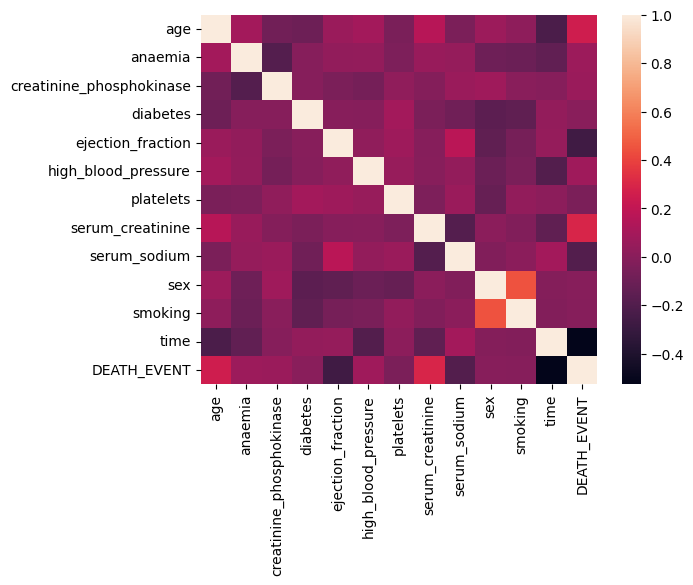
\includegraphics[width=1\linewidth]{apendices/fig/6_IAA006_1.png}
\caption{Mapa de correlação dados clínicos}
\end{figure}


\begin{lstlisting}[language=Python, style=input]
X_orig = df.iloc[:,:-1]
y_orig = df['DEATH_EVENT']

X_train_orig, X_test_orig, y_train, y_test = train_test_split(X_orig, y_orig, test_size=0.20, stratify=y_orig,random_state=10)

treinador = svm.SVC()  #algoritmo escolhido

modelo_orig = treinador.fit(X_train_orig, y_train)

# predição com os mesmos dados usados para treinar
y_pred = modelo_orig.predict(X_train_orig)
cm_orig_train = confusion_matrix(y_train, y_pred)
print('Matriz de confusao - com os dados ORIGINAIS usados no TREINAMENTO')
#print(cm_orig_train)
print(classification_report(y_train, y_pred, zero_division=0))

# predição com os mesmos dados usados para testar
y2_pred = modelo_orig.predict(X_test_orig)
cm_orig_test = confusion_matrix(y_test, y2_pred)
print('Matriz de confusao - com os dados ORIGINAIS usados para TESTES')
#print(cm_orig_test)
print(classification_report(y_test, y2_pred, zero_division=0))
\end{lstlisting}


\begin{lstlisting}[language=, style=output]
Matriz de confusao - com os dados ORIGINAIS usados no TREINAMENTO
              precision    recall  f1-score   support

           0       0.68      1.00      0.81       162
           1       0.00      0.00      0.00        77

    accuracy                           0.68       239
   macro avg       0.34      0.50      0.40       239
weighted avg       0.46      0.68      0.55       239

Matriz de confusao - com os dados ORIGINAIS usados para TESTES
              precision    recall  f1-score   support

           0       0.68      1.00      0.81        41
           1       0.00      0.00      0.00        19

    accuracy                           0.68        60
   macro avg       0.34      0.50      0.41        60
weighted avg       0.47      0.68      0.55        60
\end{lstlisting}


\begin{lstlisting}[language=Python, style=input]
y = df['DEATH_EVENT']
X = df.drop(['diabetes', 'time', 'DEATH_EVENT'],axis = 1)

X_train, X_test, y_train, y_test = train_test_split(X, y, test_size=0.20, stratify=y_orig,random_state=10)

scaler = StandardScaler().fit(X_train)
X_train_scaled = scaler.transform(X_train)
X_test_scaled = scaler.transform(X_test)

treinador = svm.SVC()  #algoritmo escolhido

modelo_orig = treinador.fit(X_train_scaled, y_train)

# predição com os mesmos dados usados para treinar
y_pred = modelo_orig.predict(X_train_scaled)
cm_orig_train = confusion_matrix(y_train, y_pred)
print('Matriz de confusao - com os dados escalonados e de alta correlacao usados no TREINAMENTO')
#print(cm_orig_train)
print(classification_report(y_train, y_pred, ))

# predição com os mesmos dados usados para testar
y2_pred = modelo_orig.predict(X_test_scaled)
cm_orig_test = confusion_matrix(y_test, y2_pred)
print('Matriz de confusao - com os dados escalonados e de alta correlacao usados no TESTE')
#print(cm_orig_test)
print(classification_report(y_test, y2_pred))
\end{lstlisting}


\begin{lstlisting}[language=, style=output]
Matriz de confusao - com os dados escalonados e de alta correlacao usados no TREINAMENTO
              precision    recall  f1-score   support

           0       0.83      0.96      0.89       162
           1       0.88      0.60      0.71        77

    accuracy                           0.85       239
   macro avg       0.86      0.78      0.80       239
weighted avg       0.85      0.85      0.84       239

Matriz de confusao - com os dados escalonados e de alta correlacao usados no TESTE
              precision    recall  f1-score   support

           0       0.78      0.85      0.81        41
           1       0.60      0.47      0.53        19

    accuracy                           0.73        60
   macro avg       0.69      0.66      0.67        60
weighted avg       0.72      0.73      0.72        60
\end{lstlisting}
\label{ap:ap07}
\chapter{Aspectos filosóficos e éticos da IA}
\section*{\textbf{A - ENUNCIADO}}
%%%%%%%%%%%NO MODELO SO VEM DPS DE VISÃO COMPUTACIONAL

\textbf{Título do Trabalho:} {\textquotedbl}Estudo de Caso: Implicações Éticas do Uso do ChatGPT{\textquotedbl}



\textbf{Trabalho em Grupo:} O trabalho deverá ser realizado em grupo de alunos de no máximo seis (06) integrantes.



\textbf{Objetivo do Trabalho:} Investigar as implicações éticas do uso do ChatGPT em diferentes contextos e propor soluções
responsáveis para lidar com esses dilemas.

\textbf{Parâmetros para elaboração do Trabalho:}



\textbf{1. Relevância Ética}: O trabalho deve abordar questões éticas significativas relacionadas ao uso da inteligência
artificial, especialmente no contexto do ChatGPT. Os alunos devem identificar dilemas éticos relevantes e explorar como
esses dilemas afetam diferentes partes interessadas, como usuários, desenvolvedores e a sociedade em geral.

\textbf{2. Análise Crítica}: Os alunos devem realizar uma análise crítica das implicações éticas do uso do ChatGPT em
estudos de caso específicos. Eles devem examinar como o algoritmo pode influenciar a disseminação de informações, a
privacidade dos usuários e a tomada de decisões éticas. Além disso, devem considerar possíveis vieses algorítmicos,
discriminação e questões de responsabilidade.

\textbf{3. Soluções Responsáveis}: Além de identificar os desafios éticos, os alunos devem propor soluções responsáveis
e éticas para lidar com esses dilemas. Isso pode incluir sugestões para políticas, regulamentações ou práticas de
design que promovam o uso responsável da inteligência artificial. Eles devem considerar como essas soluções podem
equilibrar os interesses de diferentes partes interessadas e promover valores éticos fundamentais, como transparência,
justiça e privacidade.

\textbf{4. Colaboração e Discussão}: O trabalho deve envolver discussões em grupo e colaboração entre os alunos. Eles
devem compartilhar ideias, debater diferentes pontos de vista e chegar a conclusões informadas através do diálogo e da
reflexão mútua. O estudo de caso do ChatGPT pode servir como um ponto de partida para essas discussões, incentivando os
alunos a aplicar conceitos éticos e legais aprendidos ao analisar um caso concreto.

\textbf{5. Limite de Palavras}: O trabalho terá um limite de 6 a 10 páginas teria aproximadamente entre 1500 e 3000
palavras.

\textbf{6. Estruturação Adequada}: O trabalho siga uma estrutura adequada, incluindo introdução, desenvolvimento e
conclusão. Cada seção deve ocupar uma parte proporcional do total de páginas, com a introdução e a conclusão ocupando
menos espaço do que o desenvolvimento.

\textbf{7. Controle de Informações}: Evitar incluir informações desnecessárias que possam aumentar o comprimento do
trabalho sem contribuir significativamente para o conteúdo. Concentre-se em informações relevantes, argumentos sólidos
e evidências importantes para apoiar sua análise.

\textbf{8. Síntese e Clareza}: O trabalho deverá ser conciso e claro em sua escrita. Evite repetições desnecessárias e
redundâncias. Sintetize suas ideias e argumentos de forma eficaz para transmitir suas mensagens de maneira sucinta. 

\textbf{9. Formatação Adequada}: O trabalho deverá ser apresentado nas normas da ABNT de acordo com as diretrizes
fornecidas, incluindo margens, espaçamento, tamanho da fonte e estilo de citação. Deve-se seguir o seguinte template de
arquivo: \url{https://bibliotecas.ufpr.br/wp-content/uploads/2022/03/template-artigo-de-periodico.docx}


%%%%%%%%%%%%%%%%%%%%%%%%%%%%%%%%%%%%%%%%%%%%%%%%%%%%%%%%%%%%%%%%%%%%%%%%%%%%%%%%%%%%%%%%%%%%%
\section*{\textbf{B - RESOLUÇÃO}}
\subsection*{\textbf{Estudo de Caso: Implicações Éticas do Uso do ChatGPT}}
%\noindent Caroline Pereira de Sena\\
%David Reksidler Junior \\
%Hideraldo Luis Simon Junior\\
%Marco Antonio Pedroso Vicente

\textbf{RESUMO}

O rápido avanço da inteligência artificial (IA) levou ao desenvolvimento de modelos de linguagem sofisticados como o ChatGPT. Este trabalho explora as implicações éticas do uso de tal ferramenta, focando em seu impacto em áreas como educação, ambiente de trabalho e meio artístico. Ao examinar tais estudos de caso específicos, este trabalho identificou alguns dilemas éticos significativos e analisou seus efeitos sobre diferentes partes interessadas. Além disso, o presente trabalho propõe algumas possíveis soluções responsáveis para que esses dilemas sejam superados, promovendo um uso mais positivo para a sociedade em geral. O objetivo é fornecer uma compreensão abrangente do panorama ético em torno do ChatGPT e sugerir políticas que garantam seu uso benéfico e equitativo na sociedade.

Palavras-chave: Ética. ChatGPT. Inteligência artificial. Análise crítica. Soluções responsáveis.


\textbf{ABSTRACT}

The rapid advance of artificial intelligence (AI) has led to the development of sophisticated language models such as ChatGPT. This paper explores the ethical implications of using such a tool, focusing on its impact in areas such as education, the workplace and the arts. By examining such specific case studies, this paper has identified some significant ethical dilemmas and analyzed their effects on different stakeholders. In addition, this paper proposes some possible responsible solutions so that these dilemmas can be overcome, promoting a more positive use for society in general. The aim is to provide a comprehensive understanding of the ethical landscape surrounding ChatGPT and to suggest policies that ensure its beneficial and equitable use in society.


Keywords: Ethics. ChatGPT. Artificial intelligence. Critical analysis. Responsible solutions.


\subsection*{\textbf{1 INTRODUÇÃO}}
A inteligência artificial (IA) tem evoluído rapidamente e ganhado muita popularidade recentemente. Hoje em dia, falar sobre IA é um assunto muito comum, diferente de alguns poucos anos atrás, e grande parte das pessoas acaba por utilizar serviços que utilizam inteligência artificial de alguma forma ou de outra mesmo sem saber.

Esse rápido avanço abre espaço para discussões éticas e filosóficas de como essa tecnologia pode e poderá afetar a vida das pessoas no futuro. Uma das aplicações recentes mais notáveis é o ChatGPT, uma tecnologia de IA capaz de gerar textos e realizar conversas de maneira natural. 

Este trabalho tem como objetivo explorar algumas implicações éticas do uso do ChatGPT em diversos cenários, tais como na educação, no ambiente de trabalho e também no meio artístico. Além de explorar tais implicações também investigar alguns dos dilemas que a inteligência artificial em geral apresenta hoje e por fim propor algumas soluções responsáveis para os problemas identificados.

A análise será estruturada em duas seções principais: análise crítica, onde abordaremos estudos de casos específicos para ilustrar os impactos éticos da tecnologia; e soluções responsáveis, onde serão propostas medidas para mitigar os desafios identificados e promover o uso junto e transparente do ChatGPT em tais estudos de caso. Ao realizar essa análise, esperamos contribuir para um entendimento mais profundo das implicações éticas da inteligência artificial e para o desenvolvimento de boas práticas que garantam o seu uso benéfico na sociedade, minimizando os potenciais usos negativos.

\subsection*{{1.1 CHATGPT}}
O ChatGPT é um modelo de inteligência artificial que pode entender e gerar textos como se fosse uma pessoal real. Ele foi criado para conversar com as pessoas, responder perguntas, fornecer informações e até mesmo ajudar em algumas tarefas. A tecnologia de inteligência artificial permite que o ChatGPT aprenda com diversos exemplos de conversas e textos, o que o ajuda a fornecer respostas úteis e em grande parte também corretas.

De maneira mais técnica, o ChatGPT é um modelo de linguagem treinando para gerar texto e foi otimizado para diálogos, utilizando aprendizado por reforço, com feedback humano, um método que utiliza demonstrações humanas e comparações de preferências para orientar o modelo em direção ao comportamento desejado\footnote{OPENAI. \textit{What is ChatGPT?}. Disponível em: <https://help.openai.com/en/articles/6783457-what-is-chatgpt>. Acesso em: 25 fev. 2024.}.



\subsection*{\textbf{2 ANÁLISE CRÍTICA}}
\subsection*{{2.1 ESTUDO DE CASO 1: USO NA EDUCAÇÃO}}
No contexto educacional o ChatGPT pode ser uma ferramenta valiosa para auxiliar professores no ensino dos alunos. Tal ferramenta é capaz de gerar respostas de forma rápida e diferentes, ajudando na resolução de problemas. Entretanto, há preocupações em relação ao seu uso, tanto para os corpo docente como para o discente, possibilitando a geração de um determinado nível de dependência dessa tecnologia, podendo comprometer suas capacidades intelectuais, pensamento crítico e criatividade, sem o uso da ferramenta. O processo de transformação, principalmente o digital, exige dos profissionais envolvidos com a educação, um olhar diferenciado nos planejamentos e suas respectivas aplicações, pois há muitos que são analfabetos funcionais em conduzir determinadas metodologias no processo ensino-aprendizagem, um exemplo, são as metodologias ativas, em que há uma interpretação equivocada entre gamificação e jogos. 

Nesse processo, o papel do professor não será como o de outrora em que tal personagem era a única fonte de conhecimento. Hoje e no futuro se desenham cenários em que a docência exercerá muito mais o papel de mediação pedagógica entre os objetos de conhecimento e os estudantes. Por isso, o educar pela pesquisa e extensão se tornam tão significativos\footnote{CASSOL, Daniel. \textit{Quais os impactos do ChatGPT e da Inteligência Artificial na Educação?}. Disponível em: <https://www.ifsc.edu.br/web/ifsc-verifica/w/quais-os-impactos-do-chatgpt-e-da-inteligencia-artificial-na-educacao>. Acesso em: 26 jun. 2024.}.

Para que se tenha uma qualidade na construção do saber, a entrada das informações, que devem ser interativas e desafiadoras para o aluno em  desenvolvimento para se tornar um estudante, o professor deverá estar em prontidão, não utilizando a ferramenta como “bengala” para conduzir suas aulas, bem como oferecer um suporte com maior qualidade e orientações possibilitando uma diversidade de caminhos para explorar o mundo dos saberes com consciência. Em relação aos discentes, respeitando o seu tempo de maturação na forma de perceber o mundo, fomentá-los por meio da disciplina em realizar as tarefas propostas, iniciando com uma boa orientação, sobre como aplicar a ferramenta nas determinadas áreas, utilizando a transdisciplinaridade e autoconhecimento para a ampliação da base de informações a serem utilizados na construção do pensamento crítico, sendo mais assertivo nas perguntas à serem realizadas, aumentado a probabilidade de obter melhores respostas, e na sua interpretação e execução, obter um resultado mais original, personalizado; não necessitando se utilizar do plágio ou qualquer outro artifício que não contribua com a melhoria contínua do ChatGPT, no contexto escolar e outras áreas. 


\subsection*{{2.2 ESTUDO DE CASO 2: USO NO AMBIENTE DE TRABALHO}}
No ambiente de trabalho, o uso de inteligências artificiais promete trazer um grande aumento da produtividade e precisão, além da simplificação de tarefas, o que permitiria liberar tempo para tarefas que exigem mais criatividade e pensamento crítico. O ChatGPT, nesse contexto, vem sendo visto como uma ótima ferramenta para análise de dados, organização de informações, automatização de tarefas repetitivas e geração de código, e já é amplamente popular em diversas áreas, principalmente dentro do mundo corporativo. Segundo Lopes (2024)\footnote{LOPES, André. \textit{1 em 3 profissionais no mundo usa ChatGPT no trabalho, aponta pesquisa}. Disponível em: <https://exame.com/inteligencia-artificial/1-em-cada-3-profissionais-no-mundo-usa-chatgpt-no-trabalho-aponta-pesquisa/>. Acesso em: 30 jun. 2024.}, 89\% dos profissionais de TI e 86\% do setor de marketing, já adotaram o uso do ChatGPT numa frequência, ao menos, mensal.

Apesar dos benefícios da introdução do ChatGPT no ambiente de trabalho, surgem, a partir disso, uma série de questionamentos e preocupações a respeito das mudanças que essa tecnologia pode causar. 

Uma das áreas a serem afetadas seria o mercado de trabalho, já que um dos principais questionamentos é se a ferramenta poderia ser capaz de causar a extinção de algumas carreiras. O ChatGPT parece ter o potencial de substituir pessoas na realização de algumas tarefas, como por exemplo: revisão de contratos, resumo de textos, criação de apresentações, desenvolvimento de código, organização de cadeias de produção; afetando assim profissões como direito, jornalismo, engenharia de software e magistério\footnote{SUTTO, Giovanna. \textit{ChatGPT é vilão ou oportunidade no mundo do trabalho?}. Disponível em: <https://www.infomoney.com.br/carreira/chatgpt-e-vilao-ou-oportunidade-no-mundo-do-trabalho/>. Acesso em: 30 jun. 2024.}. Apenas a remota possibilidade de que isso aconteça, poderia ser a causa do aumento do nível de ansiedade de muitos trabalhadores, talvez, gerando um problema de saúde pública. Contudo, ao mesmo tempo, há a expectativa de que surjam novas áreas de trabalho,  para profissionais especializados no uso da ferramenta, que sejam capazes de integrá-la em diferentes setores.

Além do mercado de trabalho, é válido buscar entender o efeito que o uso de ferramentas como o ChatGPT teria sobre o perfil dos trabalhadores. É importante cogitar que a intensificação do uso do ChatGPT poderá afetar as habilidades dos trabalhadores, no sentido de que ao depender muito da ferramenta como uma “muleta”, os profissionais acabem “atrofiando” suas habilidades. Poderia haver diminuição na habilidade de comunicação escrita, pois o uso da IA para gerar conteúdos textuais em alta frequência reduz o não aprimoramento e o esquecimento de técnicas de escrita. Por sua vez, a redução da habilidade de comunicação escrita também tem impacto na comunicação verbal, pois afeta a habilidade de formulação de argumentos e organização de idéias, e então pode ser a causa de mais problemas de comunicação no ambiente de trabalho. 

A inibição da criatividade também poderia ser uma outra consequência, visto que o uso do ChatGPT ajuda na otimização de produção de texto inédito porém não gera conhecimento novo, considerando que é treinado com conhecimento produzido no passado. A tendência é que o conteúdo produzido pelo uso recorrente do ChatGPT gere uma repetição ou reprodução de informações entre os profissionais, em variados setores e sem avanço ou melhoria. Em nome da otimização do tempo, a inovação é inibida e se diminui o hábito e o exercício da criatividade.

Surge também a dúvida sobre até que ponto uma inteligência artificial pode ser utilizada em tarefas que dependem de pesquisa e consulta a informações verdadeiras. Com uma compreensão mais aprofundada do funcionamento de inteligências artificiais, sabe-se que elas não são capazes de raciocinar, compreender o contexto e aspectos humanos relacionados, apenas são capazes de abstrair dados e são capazes de gerar dados fictícios quando não possuem as informações verdadeiras. Porém ferramentas como o ChatGPT passaram a ser usadas por muitos como uma fonte fácil de conhecimento verdadeiro, o que gera a necessidade de treinar profissionais para aprender a usar a ferramenta e analisar criticamente se o conteúdo gerado é válido ou não.

O aspecto da experiência do usuário também passa a ser afetado, devido ao aumento de ferramentas automatizadas para atendimento aos clientes. Não é incomum, ao acessar o site de uma empresa e ao se direcionar para o serviço de atendimento ao cliente, o mesmo ser redirecionado para uma conversa com robôs. Tais robôs em grande maioria se utilizam de ferramentas geradoras de textos como o ChatGPT para se comunicarem e auxiliarem na resolução de problemas comuns entre clientes de uma determinada empresa. Isso de certa forma pode melhorar a eficiência de diversos atendimentos, fornecendo respostas rápidas e quase sempre precisas. Entretanto, embora leve a um aumento na eficiência operacional do atendimento, muitas pessoas reclamam da “desumanização” nesses processos, onde os clientes geralmente sentem falta de interações humanas autênticas, principalmente se tratando de problemas mais complexos que nem sempre os robôs conseguem ajudar. 


\subsection*{{2.3 ESTUDO DE CASO 3: USO NO MEIO ARTÍSTICO}}
A inteligência artificial tem sido cada vez mais utilizada em diversas áreas criativas para a produção de novas artes, desde músicas até pinturas ou histórias. O ChatGPT em específico com sua enorme capacidade em gerar textos pode ser utilizado para criação de livros, roteiros, poesias, letras de músicas e até mesmo colaborar criativamente na criação de outros tipos de obras de arte. Para fins de simplicidade no texto chamaremos qualquer produção artística de obra. 

Apesar dos erros e falhas ainda presentes, a habilidade já demonstrada pelo chat e seu potencial de se aprimorar ainda mais no futuro vem gerando não apenas admiração, mas também alguns receios\footnote{SUZUKI, Shin. \textit{O que é ChatGPT e por que alguns o veem como ameaça}. Disponível em: <https://www.bbc.com/portuguese/geral-64297796>. Acesso em: 24 jun. 2024.}. Este estudo de caso examina as implicações éticas do uso do ChatGPT no meio artístico, analisando como tal tecnologia influencia a criatividade humana, a originalidade, os direitos autorais e a autenticidade das obras de artes.

Conforme brevemente citado anteriormente, o ChatGPT pode ser utilizado no meio artístico para várias finalidades como:

\begin{itemize}
    \item Criação de histórias e roteiros: Escritores ou até mesmo cineastas podem utilizar a ferramenta para gerar diálogos, desenvolver roteiros e histórias, séries ou peças de teatro.
    \item Poesia e literatura: Poetas e escritores podem obter auxílio do ChatGPT para criar poemas, contos e romances.
    \item Composição musical: Músicos podem utilizar a ferramentas para escrever letras de música ou até mesmo compor melodias.
    \item Artes visuais: Artistas podem utilizar de um auxílio criativo do chat para gerar descrições e conceitos de obras de artes que podem ser transformados em arte visual.
\end{itemize}

A principal preocupação ética relacionada ao uso de inteligência artificial no meio artístico é a respeito da originalidade dos conteúdos gerados. A arte tradicionalmente valoriza a expressão individual e criativa que existe em cada ser humano, o uso de um modelo de inteligência artificial que é treinado a partir de obras já existentes rompe com essa tradição. Se uma obra é criada totalmente ou com certa assistência do ChatGPT, até que ponto ela pode ser considerada uma expressão genuína de um artista humano?

Partindo da preocupação anterior, além da originalidade artística, outro ponto a se considerar é o dos direitos autorais. Tais obras geradas criam enormes desafios para a determinação de autoria de propriedade intelectual. De maneira geral, se uma IA contribui para a criação de uma obra, quem deve ser creditado como autor? O desenvolvedor da IA, o usuário que a utilizou, ambos, ou os autores a qual o modelo se baseou durante o treinamento?

Além dessa preocupação com direitos autorais na criação de uma obra nova, também há a preocupação sobre a violação de direitos autorais sobre obras já existentes, tendo em vista que os modelos são treinados sobre um conjunto já existente de obras. Isso levanta a questão de possível infração de direito autoral já que o modelo pode gerar conteúdo semelhante a essas obras. E neste caso novamente fica a pergunta, quem deve ser responsabilizado? Em várias partes do mundo cresce um movimento que defende mudanças nas leis de direitos autorais para que elas passem a proteger as obras dos artistas humanos das obras geradas por inteligência artificial\footnote{PRADO, Carol. \textit{ChatGPT e direito autoral: Entenda a treta jurídica que ronda a relação entre inteligência artificial e arte}. Disponível em: <https://g1.globo.com/pop-arte/noticia/2023/04/11/chatgpt-e-direito-autoral-entenda-a-treta-juridica-que-ronda-a-relacao-entre-inteligencia-artificial-e-arte.ghtml>. Acesso em: 23 jun. 2024.}. 


\subsection*{\textbf{3 SOLUÇÕES RESPONSÁVEIS}}
\subsection*{{3.1 PRIVACIDADE}}
Como toda tecnologia emergente, na Inteligência Artificial Generativa existem riscos em sua utilização. Uma das preocupações do uso generalizado desta tecnologia é o impacto na privacidade de dados. Desta forma, “para colher os benefícios dessa tecnologia inovadora, é crucial construir uma relação de confiança com o mercado e com os diversos \textit{stakeholders}, diminuindo preocupações a respeito de como os dados serão utilizados.”\footnote{KPMG. \textit{O desafio da privacidade em um mundo com crescente uso de IA}. Disponível em: <https://kpmg.com/br/pt/home/insights/2023/12/desafio-privacidade-mundo-crescente-uso-ia.html>. Acesso em: 29 jul. 2024.}

O movimento de órgãos reguladores é essencial para balizar o uso e definir os direitos e deveres. Por exemplo, o Parlamento Europeu publicou, em 2023, o AI Act e no Brasil estamos discutindo através do Projeto de Lei nº 2338, de 2023 (\url{https://www25.senado.leg.br/web/atividade/materias/-/materia/157233}). Com os balizadores criados diminui-se as preocupações, tanto dos usuários, quanto dos stackholders. Garantindo aos usuários o controle e a consciência de como seus dados serão utilizados e possibilitando o crescimento exponencial no uso da tecnologia. 

\subsection*{{3.2 TRANSPARÊNCIA}}
Embora alguns modelos tenham uma certa natureza imprevisível, a transparência dos processos que ocorrem durante o treinamento e utilização de modelos geradores de texto são essenciais para construir a confiança dos usuários. 

As empresas que desenvolvem esse tipo de tecnologia devem ser transparentes quanto a como seus modelos funcionam, incluindo detalhes sobre os dados utilizados para treinamento e os processos de tomada de decisão.

Utilizando como exemplo a AI Act, publicada em 2023, pelo Parlamento Europeu, temos a seguinte diretriz:

“A IA generativa, como o ChatGPT, não será classificada como de alto risco, mas terá que cumprir os requisitos de transparência e a lei de direitos autorais da UE:

\begin{itemize}
    \item Divulgar que o conteúdo foi gerado por IA.
    \item Projetar o modelo para evitar a geração de conteúdo ilegal.
    \item Publicação de resumos de dados protegidos por direitos autorais usados para treinamento\footnote{EUROPEAN PARLIAMENT (EP). \textit{EU AI Act: first regulation on artificial intelligence}. Disponível em: <https://www.europarl.europa.eu/thinktank/en/document/EPRS\_BRI\(2021\)698792>. Acesso em: 29 jul. 2024.}.
\end{itemize}

Para o uso de transparência nos modelos, existem projetos open sources que facilitam a implantação, como o TrustyAI (\url{https://github.com/trustyai-explainability}).

\subsection*{{3.3 VIESES}}
O viés de IA é como chamamos a ocorrência de resultados tendenciosos devido a vieses que distorcem os dados de treinamentos levando a resultados distorcidos. Na prática, os modelos absorvem preconceitos humanos, através das bases de treinamento, e os reproduzem em seus resultados.

Há uma série de vieses possíveis em um modelo de IA. Segundo o artigo “O que é viés de IA?”\footnote{IBM. \textit{O que é viés de IA?}. Disponível em: <https://www.ibm.com/br-pt/topics/ai-bias>. Acesso em: 29 jun. 2024.} temos os seguintes tipos:

\begin{itemize}
\item Viés do algoritmo
\item Viés cognitivo
\item Viés de confirmação
\item Viés de exclusão
\item Viés de medição
\item Viés de homogeneidade fora do grupo
\item Viés de preconceito
\item Viés de recordação
\item Viés de amostragem/seleção
\item Viés de estereótipo 
\end{itemize}

Para que a IA não possua vieses é necessário analisar os dados de treinamentos e tomar medidas para a diversidade dos dados, garantindo dados completos, imparciais e sem preconceitos. 


\subsection*{\textbf{4 CONCLUSÃO}}
A inteligência artificial representa um grande avanço tecnológico para a humanidade. O uso do ChatGPT em específico trouxe inúmeros benefícios capazes de transformar diversos setores da nossa sociedade, desde ambientes educacionais até meios artísticos. No entanto, com grandes poderes vêm grandes responsabilidades, e essa ferramenta poderosa também levanta questões éticas importantes a serem discutidas.

Ao longo deste trabalho exploramos somente algumas dessas implicações éticas, e analisamos como essas implicações afetam diferentes partes interessadas, desde usuários, desenvolvedores e a sociedade em geral. Além disso, propusemos algumas soluções que podem ajudar a mitigar os problemas apresentados, promovendo um uso mais positivo, justo, transparente e ético da tecnologia.

É essencial que continuemos discutindo e desenvolvendo políticas, visando a garantia que a evolução da inteligência artificial esteja sempre alinhada com princípios éticos, tendo em vista a forte tendência de que a velocidade da evolução aumente cada vez mais. Somente assim poderemos, como sociedade, aproveitar todo o potencial que essa tecnologia tem a oferecer.
\label{ap:ap08}
\chapter{Aprendizado de máquina}
\section*{\textbf{A - ENUNCIADO}}
Para cada uma das tarefas abaixo (Classificação, Regressão etc.) e cada base de dados (Veículo, Diabetes etc.), fazer os
experimentos com todas as técnicas solicitadas (KNN, RNA etc.) e preencher os quadros com as estatísticas solicitadas,
bem como os resultados pedidos em cada experimento.

%%%%%%%%%%%%%%%%%%%%%%%%%%%%%%%%%%%%%%%%%%%%%%%%%%%%%%%%%%%%%%%%%%%%%%%%%%%%%%%%%%%%%%%%%%%%%
\section*{\textbf{B - RESOLUÇÃO}}
\begin{adjustwidth}{1em}{}
\textbf{Classificação}
\end{adjustwidth}

\begin{quote}
Para o experimento de Classificação:
\begin{itemize}
    \item Ordenar pela Acurácia (descendente), ou seja, a técnica de melhor
acurácia ficará em primeiro na tabela.
    \item Após o quadro colocar:
    \begin{itemize}
        \item Um resultado com 3 linhas com a predição de novos casos para a
técnica/parâmetro de maior Acurácia (criar um arquivo com novos casos à
sua escolha)
        \item A lista de comandos emitidos no RStudio para conseguir os resultados
obtidos
    \end{itemize}
\end{itemize}
\end{quote}

\begin{center}
    \textbf{Veículo}
\end{center}


\begin{longtable}{|>{\centering\arraybackslash}p{2.5cm}|>{\centering\arraybackslash}m{2.5cm}|c|m{7cm}|}
\caption{\mbox{Resultados da classificação na base de veículos}} \\
\hline
\textbf{Técnica} & \textbf{Parâmetro} & \textbf{Acurácia} & \textbf{Matriz de Confusão} \\
\hline
\endfirsthead

\hline
\textbf{Técnica} & \textbf{Parâmetro} & \textbf{Acurácia} & \textbf{Matriz de Confusão} \\
\hline
\endhead

\hline
\colorbox[HTML]{CAF2C2}{SVM - CV} & C=100 Sigma=0.015 & \colorbox[HTML]{CAF2C2}{0.8623} & 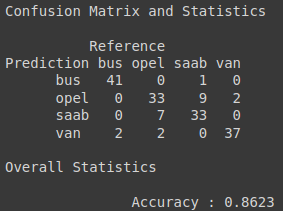
\includegraphics[width=0.4\textwidth]{apendices/fig/8_IAA008_1.png} \\
\hline
RNA - CV  & size=31 decay=0.4 & 0.8443 & 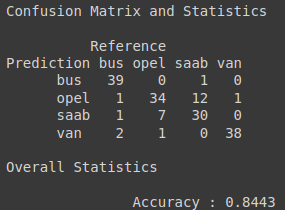
\includegraphics[width=0.4\textwidth]{apendices/fig/8_IAA008_2.png} \\
\hline
SVM - Hold-out  & C=1 Sigma= 0.0661018 & 0.7665 & 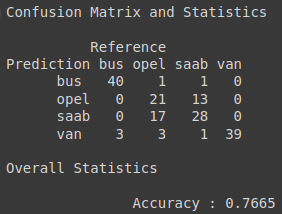
\includegraphics[width=0.4\textwidth]{apendices/fig/8_IAA008_3.png} \\
\hline
RF - CV   & mtry=5 & 0.7964 & 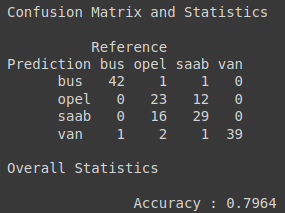
\includegraphics[width=0.4\textwidth]{apendices/fig/8_IAA008_4.png} \\
\hline
RF - Hold-out    & mtry=2 & 0.7844 & 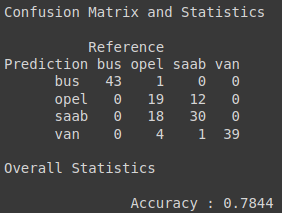
\includegraphics[width=0.4\textwidth]{apendices/fig/8_IAA008_5.png} \\
\hline
KNN    & k=3 & 0.7 & 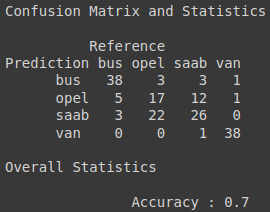
\includegraphics[width=0.4\textwidth]{apendices/fig/8_IAA008_6.png} \\
\hline
RNA - Hold-out    & size=3 decay=0.1 & 0.6287 & 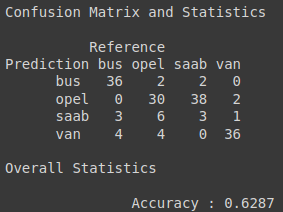
\includegraphics[width=0.4\textwidth]{apendices/fig/8_IAA008_7.png} \\
\hline
\caption*{Fonte: O autor (2024).}
\end{longtable}


\begin{center}
    \textbf{Predição novos casos (SVM - CV)}
\end{center}

\begin{table}[H]
\caption{Resultados predição novos casos (SVM - CV) - Parte 1}
\hspace*{-1.5cm} % shift left (adjust as needed)
\begin{minipage}{\textwidth}
\centering
\begin{tabular}{|c|c|c|c|c|c|c|c|c|c|}
\hline
Comp & Circ & DCirc & RadRa & PrAxisRa & MaxLRa & ScatRa & Elong & PrAxisRect & MaxLRect \\
\hline
84   & 53   & 89    & 170   & 75       & 7      & 153    & 45    & 20         & 165 \\
\hline
87   & 35   & 90    & 450   & 57       & 8      & 160    & 50    & 15         & 165 \\
\hline
100  & 40   & 100   & 205   & 60       & 11     & 210    & 35    & 30         & 165 \\
\hline
\end{tabular}
\end{minipage}
\caption*{Fonte: O autor (2024).}
\end{table}

\begin{table}[H]
\caption{Resultados predição novos casos (SVM - CV) - Parte 2 }
\hspace*{-2.5cm} % shift left (adjust as needed)
\begin{minipage}{\textwidth}
\centering
\begin{tabular}{|c|c|c|c|c|c|c|c|c|}
\hline
ScVarMaxis & ScVarmaxis & RaGyr & SkewMaxis & Skewmaxis & Kurtmaxis & KurtMaxis & HollRa & svm \\
\hline
170 & 350 & 180 & 65 & 8  & 15 & 180 & 197 & van \\
\hline
170 & 315 & 154 & 55 & 10 & 12 & 190 & 196 & opel \\
\hline
220 & 625 & 200 & 75 & 11 & 10 & 185 & 195 & saab \\
\hline
\end{tabular}
\end{minipage}
\caption*{Fonte: O autor (2024).}
\end{table}


\begin{center}
    \textbf{Lista de comandos (SVM - CV)}
\end{center}

\begin{lstlisting}[language=R, style=input]
install.packages("e1071")
install.packages("caret")
install.packages("mlbench")
install.packages("mice")
install.packages("Metrics")
install.packages("kernlab")
library("caret")
library("mlbench")
library("mice")
library("Metrics")
setwd("/content")
seed_padrao <- 202412

dados <- read.csv("6 - Veiculos - Dados.csv")
dados$a <- NULL
View(dados)

set.seed(seed_padrao)
indices <- createDataPartition(dados$tipo, p=0.80, list=FALSE)
treino <- dados[indices,]
teste <- dados[-indices,]

ctrl <- trainControl(method = "cv", number = 10)
grid <- expand.grid(C=c(1, 2, 10, 50, 100), sigma=c(.01, .015,
0.2))
set.seed(seed_padrao)
svm <- train(form = tipo~. , data = treino , method = "svmRadial" ,
tuneGrid = grid , trControl = ctrl)
svm

predict.svm <- predict(svm, teste)
confusionMatrix(predict.svm, as.factor(teste$tipo))

dados_novos_casos <- read.csv("6 - Veiculos - Dados - Novos
Casos.csv")
dados_novos_casos$a <- NULL
View(dados_novos_casos)

predict.svm <- predict(svm, dados_novos_casos)
resultado <- cbind(dados_novos_casos, predict.svm)
resultado$tipo <- NULL
View(resultado)
\end{lstlisting}

\newpage
\begin{center}
    \textbf{Diabetes}
\end{center}


\begin{longtable}{|>{\centering\arraybackslash}p{3cm}|>{\centering\arraybackslash}m{2.5cm}|c|m{7cm}|}
\caption{\mbox{Resultados da classificação na base de diabetes}} \\
\hline
\textbf{Técnica} & \textbf{Parâmetro} & \textbf{Acurácia} & \textbf{Matriz de Confusão} \\
\hline
\endfirsthead

\hline
\textbf{Técnica} & \textbf{Parâmetro} & \textbf{Acurácia} & \textbf{Matriz de Confusão} \\
\hline
\endhead

\hline
\colorbox[HTML]{CAF2C2}{SVM Hold-out} & C=0.5 Sigma= 0.1219692 & \colorbox[HTML]{CAF2C2}{0.7843} & 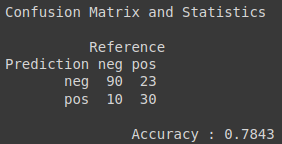
\includegraphics[width=0.4\textwidth]{apendices/fig/8_IAA008_8.png} \\
\hline
\colorbox[HTML]{CAF2C2}{SVM - CV} & C=0.5 Sigma= 0.1219692 & \colorbox[HTML]{CAF2C2}{0.7843} & 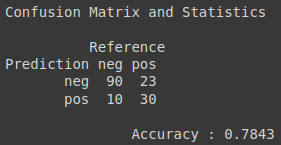
\includegraphics[width=0.4\textwidth]{apendices/fig/8_IAA008_9.png} \\
\hline
RNA - CV & size=11 decay=0.4 & 0.7778 & 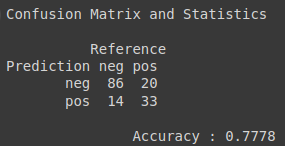
\includegraphics[width=0.4\textwidth]{apendices/fig/8_IAA008_10.png} \\
\hline
KNN & k=9 & 0.7727 & 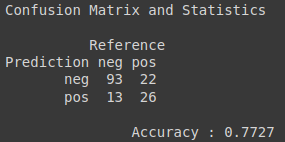
\includegraphics[width=0.4\textwidth]{apendices/fig/8_IAA008_11.png} \\
\hline
RF - Hold-out & mtry=2 & 0.7647 & 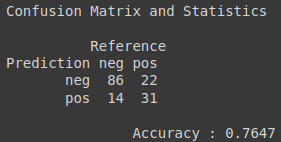
\includegraphics[width=0.4\textwidth]{apendices/fig/8_IAA008_12.png} \\
\hline
RF - CV  & mtry=8 & 0.7582 & 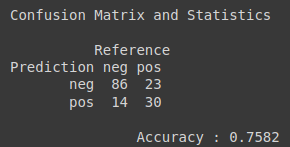
\includegraphics[width=0.4\textwidth]{apendices/fig/8_IAA008_13.png} \\
\hline
RNA Hold-out  & size=5 decay=0.1 & 0.7386 & 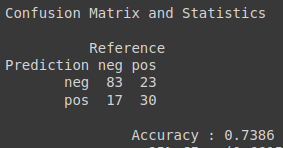
\includegraphics[width=0.4\textwidth]{apendices/fig/8_IAA008_14.png} \\
\hline
\caption*{Fonte: O autor (2024).}
\end{longtable}


\begin{center}
    \textbf{Predição novos casos (SVM Hold-out)}
\end{center}

\begin{table}[H]
\centering
\caption{Resultados da predição novos casos (SVM Hold-out)}
\begin{tabular}{|c|c|c|c|c|c|c|c|c|}
\hline
preg0nt & glucose & pressure & triceps & insulin & mass & pedigree & age & predict.svm \\
\hline
8 & 140 & 80 & 30 & 0 & 40.5 & 500 & 45 & neg \\
\hline
8 & 120 & 50 & 40 & 0 & 20.7 & 625 & 35 & neg \\
\hline
2 & 50  & 60 & 25 & 0 & 30.3 & 544 & 32 & neg \\
\hline
\end{tabular}
\caption*{Fonte: O autor (2024).}
\end{table}

\begin{center}
    \textbf{Lista de comandos (SVM Hold-out)}
\end{center}

\begin{lstlisting}[language=R, style=input]
install.packages("e1071")
install.packages("caret")
install.packages("mlbench")
install.packages("mice")
install.packages("Metrics")
install.packages("kernlab")
library("caret")
library("mlbench")
library("mice")
library("Metrics")

setwd("/content")
seed_padrao <- 202412

temp_dados <- read.csv("10 - Diabetes - Dados.csv")
temp_dados$num <- NULL
imp <- mice(temp_dados)
dados <- complete(imp, 1)
View(dados)

set.seed(seed_padrao)
indices <- createDataPartition(dados$diabetes, p=0.80,list=FALSE)
treino <- dados[indices,]
teste <- dados[-indices,]

set.seed(seed_padrao)
svm <- train(diabetes~., data=treino, method="svmRadial")
svm

predict.svm <- predict(svm, teste)
confusionMatrix(predict.svm, as.factor(teste$diabetes))

dados_novos_casos <- read.csv("10 - Diabetes - Dados - Novos
Casos.csv")
dados_novos_casos$num <- NULL
View(dados_novos_casos)

predict.svm <- predict(svm, dados_novos_casos)
resultado <- cbind(dados_novos_casos, predict.svm)
resultado$diabetes <- NULL
View(resultado)
\end{lstlisting}


\begin{adjustwidth}{1em}{}
\textbf{Regressão}
\end{adjustwidth}

\begin{quote}
Para o experimento de Regressão:
\begin{itemize}
    \item Ordenar por R2 descendente, ou seja, a técnica de melhor R2 ficará em primeiro na tabela.
    \item Após o quadro colocar:
    \begin{itemize}
        \item Um resultado com 3 linhas com a predição de novos casos para a técnica/parâmetro de maior R2 (criar um arquivo com novos casos à sua escolha)
        \item O Gráfico de Resíduos para a técnica/parâmetro de maior R2
        \item A lista de comandos emitidos no RStudio para conseguir os resultados obtidos
    \end{itemize}
\end{itemize}
\end{quote}

\newpage
\begin{center}
    \textbf{Admissão}
\end{center}


\begin{table}[H]
\caption{Resultados da regressão na base de admissão}
\hspace*{-1.5cm} 
\begin{minipage}{\textwidth}
\centering
{\renewcommand{\arraystretch}{1.7} % vertical padding
 %\setlength{\tabcolsep}{8pt}       % horizontal padding

\begin{tabular}{|c|p{3cm}|p{2cm}|p{2cm}|p{2cm}|p{2cm}|p{2cm}|}
\hline
\textbf{Técnica} & \textbf{Parâmetro} & \textbf{R2} & \textbf{Syx} & \textbf{Pearson} & \textbf{Rmse} & \textbf{MAE} \\
% \hline
% \colorbox[HTML]{CAF2C2}{SVM - CV} & C=2 Sigma=0.01 & \colorbox[HTML]{CAF2C2}{\makecell[l]{0.8882\\227024\\50831}} & \colorbox[HTML]{CAF2C2}{\makecell[l]{0.04632\\915579\\36475}} & \colorbox[HTML]{CAF2C2}{\makecell[l]{0.94268\\843613\\8658}} & \colorbox[HTML]{CAF2C2}{\makecell[l]{0.0441\\50573\\78381\\55}} & \colorbox[HTML]{CAF2C2}{\makecell[l]{0.0332\\09194\\19084\\42}} \\
% \hline
% SVM - Hold-out & C=1 Sigma= 0.2004666 & \makecell[l]{0.8676\\446382\\09649} & \makecell[l]{0.05041\\367457\\36519} & \makecell[l]{0.93174\\345191\\1874} & \makecell[l]{0.0480\\43022\\17141\\79} & \makecell[l]{0.0362\\44211\\18180\\7} \\
% \hline
% RF - Hold-out  & mtry=2 & \makecell[l]{0.8609\\300253\\48176} & \makecell[l]{0.05167\\664040\\73779} & \makecell[l]{0.93087\\499063\\6073} & \makecell[l]{0.0492\\46598\\30556\\37} & \makecell[l]{0.0368\\19141\\50290\\51} \\
% \hline
% RF - CV  & mtry=2 & \makecell[l]{0.8609\\300253\\48176} & \makecell[l]{0.05167\\664040\\73779} & \makecell[l]{0.93087\\499063\\6073} & \makecell[l]{0.0492\\46598\\30556\\37} & \makecell[l]{0.0368\\19141\\50290\\51} \\
% \hline
% RNA - CV  & size=5 decay=0.1 & \makecell[l]{0.8391\\787415\\23624} & \makecell[l]{0.05557\\114075\\7806} & \makecell[l]{0.91931\\808890\\1637} & \makecell[l]{0.0529\\57963\\68935\\19} & \makecell[l]{0.0435\\61868\\14603\\77} \\
% \hline
% RNA - Hold-out  & size=5 decay=0.1 & \makecell[l]{0.8293\\968576\\03891} & \makecell[l]{0.05723\\624012\\77942} & \makecell[l]{0.91489\\468169\\6537} & \makecell[l]{0.0545\\44763\\43419\\27} & \makecell[l]{0.0454\\27406\\52315\\09} \\
% \hline
% KNN  & K=9  & \makecell[l]{0.7773\\387140\\24105} & \makecell[l]{0.06538\\828402\\4072} & \makecell[l]{0.88345\\699730\\2136} & \makecell[l]{0.0623\\13465\\65563\\19} & \makecell[l]{0.0481\\85941\\04308\\39} \\
\hline%%%%%%%%%%%%%%%%%%%%%%%%%%%%%%%%%%%%%
\colorbox[HTML]{CAF2C2}{SVM - CV} & C=2 Sigma=0.01 & \colorbox[HTML]{CAF2C2}{0.8882} & \colorbox[HTML]{CAF2C2}{0.0463} & \colorbox[HTML]{CAF2C2}{0.9427} & \colorbox[HTML]{CAF2C2}{0.0442} & \colorbox[HTML]{CAF2C2}{0.0332} \\
\hline
SVM - Hold-out & C=1 Sigma= 0.2004666 & 0.8676 & 0.0504 & 0.9317 & 0.0480 & 0.0362 \\
\hline
RF - Hold-out & mtry=2 & 0.8609 & 0.0517 & 0.9309 & 0.0492 & 0.0368 \\
\hline
RF - CV & mtry=2 & 0.8609 & 0.0517 & 0.9309 & 0.0492 & 0.0368 \\
\hline
RNA - CV & \makecell[l]{size=5\\decay=0.1} & 0.8392 & 0.0556 & 0.9193 & 0.0529 & 0.0436 \\
\hline
RNA - Hold-out & \makecell[l]{size=5\\decay=0.1} & 0.8294 & 0.0572 & 0.9149 & 0.0545 & 0.0454 \\
\hline
KNN & K=9 & 0.7773 & 0.0654 & 0.8835 & 0.0623 & 0.0482 \\
\hline
\end{tabular}
}
\end{minipage}
\caption*{Fonte: O autor (2024).}
\end{table}


\begin{center}
    \textbf{Predição novos casos (SVM - CV)}
\end{center}

\begin{table}[H]
\centering
\caption{Resultados da predição novos casos (SVM - CV)}
\begin{tabular}{|c|c|c|c|c|c|c|c|}
\hline
GRE.S & TOEFL.S & University.R & SOP & LOR & CGPA & Research & predict \\
\hline
300 & 125 & 3 & 4.5 & 4.5 & 8.87 & 1 & 0.7948 \\
\hline
350 & 99 & 4 & 3.0 & 3.0 & 9.00 & 1 & 0.8113 \\
\hline
325 & 85 & 4 & 4.5 & 3.5 & 8.75 & 1 & 0.7042 \\
\hline
\end{tabular}
\caption*{Fonte: O autor (2024).}
\end{table}


\begin{center}
    \textbf{Gráfico de resíduos (SVM - CV)}
\end{center}

\begin{figure}[H]
\centering
\caption{Gráfico de resíduos (SVM - CV)}
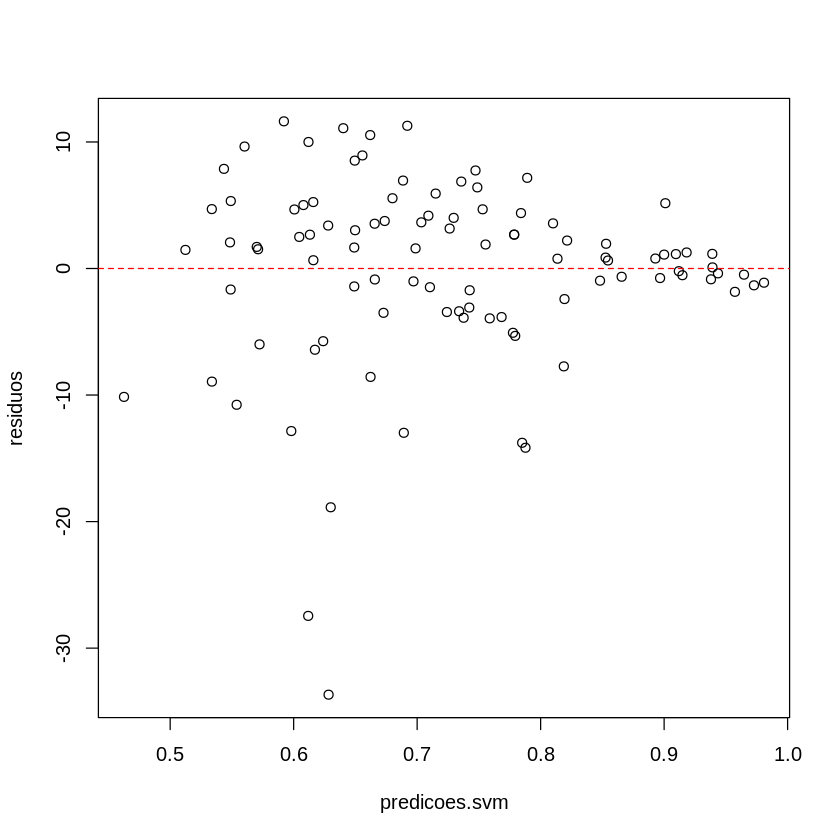
\includegraphics[width=.8\linewidth]{apendices/fig/8_IAA008_15.png}
\caption*{Fonte: O autor (2024).}
\end{figure}

\begin{center}
    \textbf{Lista de comandos (SVM – CV)}
\end{center}


\begin{lstlisting}[language=R, style=input]
install.packages("e1071")
install.packages("caret")
install.packages("mlbench")
install.packages("mice")
install.packages("Metrics")
install.packages("kernlab")
library("caret")
library("mlbench")
library("mice")
library("Metrics")

setwd("/content")
seed_padrao <- 202412

dados <- read.csv("9 - Admissao - Dados.csv", header=T)
dados$num <- NULL
View(dados)

set.seed(seed_padrao)
indices <- createDataPartition(dados$ChanceOfAdmit, p=0.80,
list=FALSE)
treino <- dados[indices,]
teste <- dados[-indices,]

control <- trainControl(method = "cv", number = 10)
tuneGrid <- expand.grid(C=c(1, 2, 10, 50, 100), sigma=c(.01, .015,
0.2))
set.seed(seed_padrao)
svm <- train(ChanceOfAdmit~., data=treino, method="svmRadial",
trainControl=control, tuneGrid=tuneGrid)
svm
predicoes.svm <- predict(svm, teste)

print("RMSE")
rmse(teste$ChanceOfAdmit, predicoes.svm)

print("R2")
r2 <- function(predito, observado) {
return(1 - (sum((predito-observado)^2) /
sum((observado-mean(observado))^2)))
}
r2(predicoes.svm,teste$ChanceOfAdmit)

print("SYX")
syx <- function(predito, observado, n, p)
{
sqrt((sum((observado-predito)^2))/(n-p-1))
}
syx(predicoes.svm,teste$ChanceOfAdmit, nrow(teste), ncol(teste))

print("PEARSON")
pearson <- function(predito, observado) {
n <- length(predito)
predito_media <- mean(predito)
observado_media <- mean(observado)

num <- sum((predito - predito_media) * (observado -
observado_media))
denom <- sqrt(sum((predito - predito_media)^2) * sum((observado -
observado_media)^2))

r <- num / denom
return(r)
}
pearson(predicoes.svm, teste$ChanceOfAdmit)

print("MAE")
mae <- function(predito, observado)
{
error = observado-predito
mean(abs(error))
}
mae(predicoes.svm, teste$ChanceOfAdmit)

residuos <- ((teste$ChanceOfAdmit -
predicoes.svm)/teste$ChanceOfAdmit)*100
plot(residuos ~ predicoes.svm)
abline(h = 0, lty = 2, col = "red")

dados_novos_casos <- read.csv("9 - Admissao - Dados - Novos
Casos.csv")
dados_novos_casos$num <- NULL
View(dados_novos_casos)

predict.svm <- predict(svm, dados_novos_casos)
resultado <- cbind(dados_novos_casos, predict.svm)
resultado$ChanceOfAdmit <- NULL
View(resultado)
\end{lstlisting}


\begin{center}
    \textbf{Biomassa}
\end{center}

% \begin{table}[H]
% \centering
% \caption{Resultados da regressão na base de biomassa}
% \hspace*{-3cm} % shift left (adjust as needed)
% \begin{minipage}{\textwidth}
% \begin{tabular}{|l|l|l|l|l|l|l|}
% \hline
% \textbf{Técnica} & \textbf{Parâmetro} & \textbf{R$^2$} & \textbf{Syx} & \textbf{Pearson} & \textbf{RMSE} & \textbf{MAE} \\
% \hline
% \colorbox[HTML]{CAF2C2}{RNA CV} & \makecell[l]{size=3\\decay=0.1} & \colorbox[HTML]{CAF2C2}{0.9051} & \colorbox[HTML]{CAF2C2}{821702.3177} & \colorbox[HTML]{CAF2C2}{0.9882} & \colorbox[HTML]{CAF2C2}{800372.9388} & \colorbox[HTML]{CAF2C2}{369.3600} \\
% \hline
% RNA Hold-out & \makecell[l]{size=3\\decay=0.1} & 0.8993 & 425162.0640 & 0.9751 & 215677.6934 & 380.5700 \\
% \hline
% RF Hold-out & mtry=2 & 0.8869 & 383207.4007 & 0.9852 & 47347.9748 & 403.3300 \\
% \hline
% RF CV & mtry=2 & 0.8869 & 383207.4007 & 0.9852 & 47347.9748 & 403.3300 \\
% \hline
% SVM CV & \makecell[l]{C=100\\Sigma=0.01} & 0.8091 & 401908.7333 & 0.9605 & 377289.1498 & 524.0400 \\
% \hline
% KNN & K=1 & 0.7776 & 938518.5302 & 0.9471 & 90255.5295 & 565.5700 \\
% \hline
% SVM Hold-out & \makecell[l]{C=1\\Sigma=0.8644} & 0.4750 & 264957.0777 & 0.8535 & 943243.0766 & 869.1200 \\
% \hline
% \end{tabular}
% \end{minipage}
% \end{table}
\begin{table}[H]
\caption{Resultados da regressão na base de biomassa}
\hspace*{-1.5cm} 
\begin{minipage}{\textwidth}
\centering
{\renewcommand{\arraystretch}{1.7} % vertical padding
 %\setlength{\tabcolsep}{8pt}       % horizontal padding

\begin{tabular}{|c|p{3cm}|p{2cm}|p{2cm}|p{2cm}|p{2cm}|p{2cm}|}
\hline
\textbf{Técnica} & \textbf{Parâmetro} & \textbf{R$^2$} & \textbf{Syx} & \textbf{Pearson} & \textbf{RMSE} & \textbf{MAE} \\
\hline
\colorbox[HTML]{CAF2C2}{RNA CV} & \makecell[l]{size=3\\decay=0.1} & \colorbox[HTML]{CAF2C2}{0.9051} & \colorbox[HTML]{CAF2C2}{385.7903} & \colorbox[HTML]{CAF2C2}{0.9882} & \colorbox[HTML]{CAF2C2}{369.3660} & 109.9805 \\
\hline
RNA Hold-out & \makecell[l]{size=3\\decay=0.1} & 0.8993 & 397.4928 & 0.9751 & 380.5704 & 256.7893 \\
\hline
RF Hold-out & mtry=2 & 0.8869 & 421.2733 & 0.9852 & 403.3385 & \colorbox[HTML]{CAF2C2}{102.0527} \\
\hline
RF CV & mtry=2 & 0.8869 & 421.2733 & 0.9852 & 403.3385 & \colorbox[HTML]{CAF2C2}{102.0527} \\
\hline
SVM CV & \makecell[l]{C=100\\Sigma=0.01} & 0.8091 & 547.3479 & 0.9605 & 524.0457 & 154.5247 \\
\hline
KNN & K=1 & 0.7776 & 590.7204 & 0.9471 & 565.5717 & 128.5157 \\
\hline
SVM Hold-out & \makecell[l]{C=1\\Sigma=0.8644} & 0.4750 & 907.7681 & 0.8535 & 869.1218 & 199.1633 \\
\hline
\end{tabular}
}
\end{minipage}
\caption*{Fonte: O autor (2024).}
\end{table}



\begin{center}
    \textbf{Predição novos casos (RNA - CV)}
\end{center}

\begin{table}[H]
\centering
\caption{Resultado da predição novos casos (RNA - CV)}
\begin{tabular}{|r|r|r|r|}
\hline
dap & h & Me & predict.rna \\
\hline
7.0 & 4.0 & 1.04 & 82.9916 \\
\hline
8.2 & 6.0 & 1.04 & 109.7899 \\
\hline
7.5 & 5.5 & 1.04 & 98.4963 \\
\hline
\end{tabular}
\caption*{Fonte: O autor (2024).}
\end{table}


\begin{center}
    \textbf{Gráfico de resíduos (RNA – CV)}
\end{center}


\begin{figure}[H]
\centering
\caption{Gráfico de resíduos (RNA - CV)}
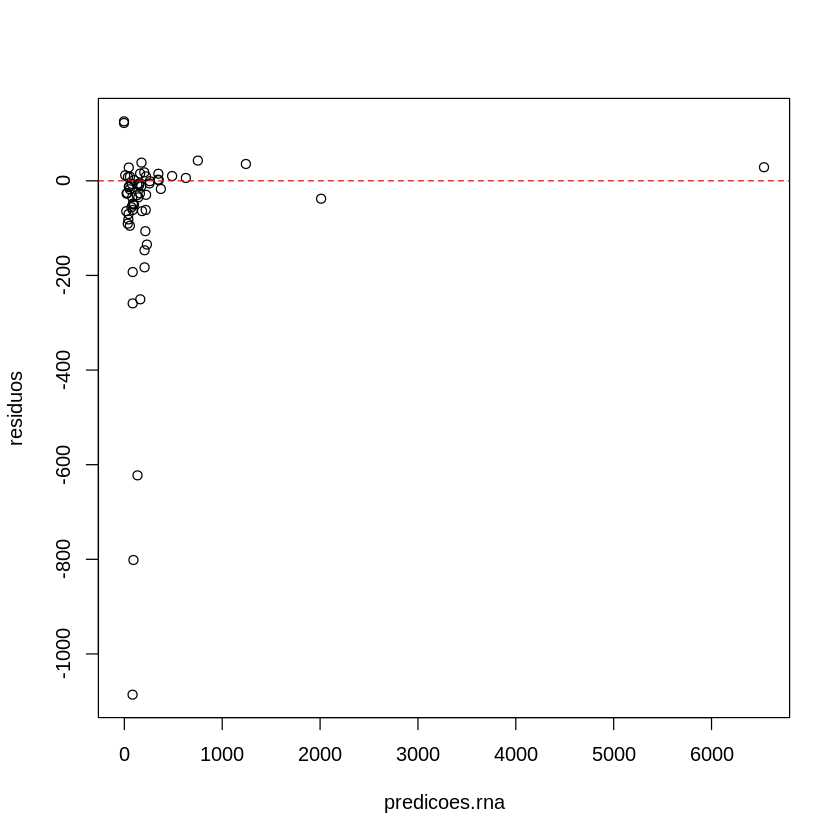
\includegraphics[width=.8\linewidth]{apendices/fig/8_IAA008_16.png}
\caption*{Fonte: O autor (2024).}
\end{figure}



\begin{center}
    \textbf{Lista de comandos (RNA - CV)}
\end{center}



\begin{lstlisting}[language=R, style=input]
install.packages("e1071")
install.packages("caret")
install.packages("mlbench")
install.packages("mice")
install.packages("Metrics")
library("caret")
library("mlbench")
library("mice")
library("Metrics")

setwd("/content")
seed_padrao <- 202412

dados <- read.csv("5 - Biomassa - Dados.csv")
View(dados)

set.seed(seed_padrao)
ind <- createDataPartition(dados$biomassa, p=0.80, list = FALSE)
treino <- dados[ind,]
teste <- dados[-ind,]

control <- trainControl(method = "cv", number = 10)
set.seed(seed_padrao)
rna <- train(biomassa~., data=treino, method="nnet",
trainControl=control, linout=T, MaxNWts=10000, maxit=2000, trace=F)
rna
predicoes.rna <- predict(rna, teste)

print("RMSE")
rmse(teste$biomassa, predicoes.rna)

print("R2")
r2 <- function(predito, observado) {
return(1 - (sum((predito-observado)^2) /
sum((observado-mean(observado))^2)))
}
r2(predicoes.rna,teste$biomassa)

print("SYX")
syx <- function(predito, observado, n, p)
{
sqrt((sum((observado-predito)^2))/(n-p-1))
}
syx(predicoes.rna,teste$biomassa, nrow(teste), ncol(teste))

print("PEARSON")
pearson <- function(predito, observado) {
n <- length(predito)
predito_media <- mean(predito)
observado_media <- mean(observado)

num <- sum((predito - predito_media) * (observado -
observado_media))
denom <- sqrt(sum((predito - predito_media)^2) * sum((observado -
observado_media)^2))

r <- num / denom
return(r)
}
pearson(predicoes.rna, teste$biomassa)

print("MAE")
mae <- function(predito, observado)
{
error = observado-predito
mean(abs(error))
}
mae(predicoes.rna, teste$biomassa)

residuos <- ((teste$biomassa - predicoes.rna)/teste$biomassa)*100
plot(residuos ~ predicoes.rna)
abline(h = 0, lty = 2, col = "red")

dados_novos_casos <- read.csv("5 - Biomassa - Dados - Novos
Casos.csv")
View(dados_novos_casos)

predict.rna <- predict(rna, dados_novos_casos)
resultado <- cbind(dados_novos_casos, predict.rna)
resultado$biomassa <- NULL
View(resultado)
\end{lstlisting}


\begin{adjustwidth}{1em}{}
\textbf{Agrupamento}
\end{adjustwidth}

\begin{center}
    \textbf{Veículo}
\end{center}

% --- Parte 1 ---
\begin{table}[H]
\centering
\caption{Clusters gerados - Parte 1}
\begin{tabular}{|c|c|c|c|c|c|c|c|}
\hline
Cluster & Comp & Circ & DCirc & Rad & Ra & PraxisRa & MaxLRa \\ \hline
1  & 85  & 43  & 70  & 120 & 56 & 7  & 149 \\ \hline
2  & 104 & 54  & 101 & 189 & 57 & 11 & 222 \\ \hline
3  & 89  & 45  & 72  & 166 & 59 & 7  & 154 \\ \hline
4  & 89  & 41  & 66  & 162 & 58 & 7  & 150 \\ \hline
5  & 90  & 37  & 74  & 169 & 59 & 7  & 157 \\ \hline
6  & 88  & 40  & 69  & 146 & 58 & 9  & 133 \\ \hline
7  & 101 & 53  & 108 & 197 & 60 & 11 & 214 \\ \hline
8  & 93  & 39  & 66  & 133 & 59 & 8  & 130 \\ \hline
9  & 85  & 36  & 51  & 116 & 57 & 6  & 122 \\ \hline
10 & 100 & 47  & 105 & 209 & 64 & 10 & 201 \\ \hline
\end{tabular}
\caption*{Fonte: O autor (2024).}
\end{table}

% --- Parte 2 ---
\begin{table}[H]
\centering
\caption{Clusters gerados - Parte 2}
\begin{tabular}{|c|c|c|c|c|c|c|c|}
\hline
Cluster & ScatRa & Elong & PraxisRect & MaxLRect & ScVarMaxis & ScVarmxis & RaGyr \\ \hline
1  & 45 & 19 & 143 & 170 & 327 & 171 & 81 \\ \hline
2  & 30 & 25 & 173 & 225 & 706 & 216 & 72 \\ \hline
3  & 44 & 19 & 144 & 174 & 347 & 174 & 69 \\ \hline
4  & 45 & 19 & 144 & 169 & 331 & 161 & 64 \\ \hline
5  & 43 & 20 & 131 & 189 & 363 & 186 & 72 \\ \hline
6  & 50 & 18 & 135 & 202 & 259 & 151 & 66 \\ \hline
7  & 31 & 24 & 162 & 226 & 661 & 214 & 71 \\ \hline
8  & 52 & 18 & 134 & 159 & 246 & 139 & 63 \\ \hline
9  & 57 & 17 & 125 & 137 & 196 & 123 & 85 \\ \hline
10 & 33 & 23 & 147 & 214 & 586 & 201 & 67 \\ \hline
\end{tabular}
\caption*{Fonte: O autor (2024).}
\end{table}

% --- Parte 3 ---
\begin{table}[H]
\centering
\caption{Clusters gerados - Parte 3}
\begin{tabular}{|c|c|c|c|c|c|}
\hline
Cluster & SkewMaxis & Skewmaxis & Kurtmaxis & KurtMaxis & Tipo \\ \hline
1  & 6  & 11 & 180 & 184 & bus  \\ \hline
2  & 0  & 11 & 187 & 198 & opel \\ \hline
3  & 5  & 2  & 190 & 196 & opel \\ \hline
4  & 4  & 0  & 188 & 197 & van  \\ \hline
5  & 1  & 7  & 196 & 202 & bus  \\ \hline
6  & 0  & 21 & 193 & 200 & opel \\ \hline
7  & 0  & 24 & 188 & 199 & saab \\ \hline
8  & 5  & 7  & 183 & 194 & van  \\ \hline
9  & 1  & 5  & 180 & 183 & saab \\ \hline
10 & 2  & 13 & 192 & 198 & bus  \\ \hline
\end{tabular}
\caption*{Fonte: O autor (2024).}
\end{table}

10 primeiras linhas do arquivo com o cluster correspondente:

% --- Parte 1 ---
\begin{table}[H]
\centering
\caption{Resumo do cluster correspondente - Parte 1}
\begin{tabular}{|c|c|c|c|c|c|c|c|}
\hline
Cluster & Comp & Circ & DCirc & Rad & Ra & PraxisRa & MaxLRa \\ \hline
4  & 95  & 48  & 83  & 178 & 72  & 10 & 162 \\ \hline
1  & 91  & 41  & 84  & 141 & 57  & 9  & 149 \\ \hline
10 & 104 & 50  & 106 & 209 & 66  & 10 & 207 \\ \hline
4  & 93  & 41  & 82  & 159 & 63  & 9  & 144 \\ \hline
1  & 85  & 44  & 70  & 205 & 103 & 52 & 149 \\ \hline
9  & 107 & 57  & 106 & 172 & 50  & 6  & 255 \\ \hline
1  & 97  & 43  & 73  & 173 & 65  & 6  & 153 \\ \hline
8  & 90  & 43  & 66  & 157 & 65  & 9  & 137 \\ \hline
9  & 86  & 34  & 62  & 140 & 61  & 7  & 122 \\ \hline
7  & 93  & 44  & 98  & 197 & 62  & 11 & 183 \\ \hline
\end{tabular}
\caption*{Fonte: O autor (2024).}
\end{table}

% --- Parte 2 ---
\begin{table}[H]
\centering
\caption{Resumo do cluster correspondente - Parte 2}
\begin{tabular}{|c|c|c|c|c|c|c|c|}
\hline
Cluster & ScatRa & Elong & PraxisRect & MaxLRect & ScVarMaxis & ScVarmxis & RaGyr \\ \hline
4  & 42 & 20 & 159 & 176 & 379 & 184 & 70 \\ \hline
1  & 45 & 19 & 143 & 170 & 330 & 158 & 72 \\ \hline
10 & 32 & 23 & 158 & 223 & 635 & 220 & 73 \\ \hline
4  & 46 & 19 & 143 & 160 & 309 & 127 & 63 \\ \hline
1  & 45 & 19 & 144 & 241 & 325 & 188 & 127 \\ \hline
9  & 26 & 28 & 169 & 280 & 957 & 264 & 85 \\ \hline
1  & 42 & 19 & 143 & 176 & 361 & 172 & 66 \\ \hline
8  & 48 & 18 & 146 & 162 & 281 & 164 & 67 \\ \hline
9  & 54 & 17 & 127 & 141 & 223 & 112 & 64 \\ \hline
7  & 36 & 22 & 146 & 202 & 505 & 152 & 64 \\ \hline
\end{tabular}
\caption*{Fonte: O autor (2024).}
\end{table}

% --- Parte 3 ---
\begin{table}[H]
\centering
\caption{Resumo do cluster correspondente - Parte 3}
\begin{tabular}{|c|c|c|c|c|c|}
\hline
Cluster & SkewMaxis & Skewmaxis & Kurtmaxis & KurtMaxis & Tipo \\ \hline
4  & 6  & 16 & 187 & 197 & van  \\ \hline
1  & 9  & 14 & 189 & 199 & van  \\ \hline
10 & 14 & 9  & 188 & 196 & saab \\ \hline
4  & 6  & 10 & 199 & 207 & van  \\ \hline
1  & 9  & 11 & 180 & 183 & bus  \\ \hline
9  & 5  & 9  & 181 & 183 & bus  \\ \hline
1  & 13 & 1  & 200 & 204 & bus  \\ \hline
8  & 3  & 3  & 193 & 202 & van  \\ \hline
9  & 2  & 14 & 200 & 208 & van  \\ \hline
7  & 4  & 14 & 195 & 204 & saab \\ \hline
\end{tabular}
\caption*{Fonte: O autor (2024).}
\end{table}



\begin{center}
    \textbf{Lista de comandos emitidos}
\end{center}


\begin{lstlisting}[language=R, style=input]
install.packages("klaR")
library(klaR)

setwd("/content")
seed_padrao <- 202412

dados <- read.csv("6 - Veiculos - Dados.csv")
dados$a <- NULL
View(dados)

set.seed(seed_padrao)
cluster.results <- kmodes(dados, 10, iter.max = 10, weighted =
FALSE )
cluster.results

resultado <- cbind(dados, cluster.results$cluster)
resultado
\end{lstlisting}


\begin{adjustwidth}{1em}{}
\textbf{Regras de associação}
\end{adjustwidth}

\begin{center}
    \textbf{Musculação}
\end{center}

Regras geradas com uma configuração de Suporte e Confiança.


\begin{figure}[H]
\centering
\caption{Resultados regras de associação}
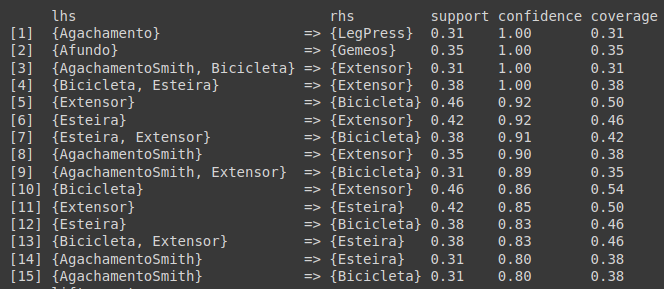
\includegraphics[width=\linewidth]{apendices/fig/8_IAA008_17.png}
\caption*{Fonte: O autor (2024).}
\end{figure}

\begin{center}
    \textbf{Lista de comandos emitidos}
\end{center}


\begin{lstlisting}[language=R, style=input]
install.packages('arules', dep=T)
library(arules)
library(datasets)

setwd("/content")
seed_padrao <- 202412

dados <- read.transactions(file="2 - Musculacao - Dados.csv",
format="basket", sep=";")
inspect(dados[1:4])

set.seed(seed_padrao)
rules <- apriori(dados, parameter = list(supp = 0.3, conf = 0.75,
minlen = 2))
summary(rules)

options(digits=2)
inspect(sort(rules, by="confidence"))
\end{lstlisting}
\label{ap:ap09}
\chapter{Deep learning}
\section*{\textbf{A - ENUNCIADO}}

\subsection*{\textbf{1 Classificação de Imagens (CNN)}}



Implementar o exemplo de classificação de objetos usando a base de dados CIFAR10 e a arquitetura CNN vista no curso.



\subsection*{\textbf{2 Detector de SPAM (RNN)}}



\textcolor{black}{Implementar o detector de spam visto em sala, usando a base de dados SMS Spam e arquitetura de RNN
vista no curso.}



\subsection*{\textbf{3 Gerador de Dígitos Fake (GAN)}}



\textcolor{black}{Implementar o gerador de dígitos }\textit{\textcolor{black}{fake}}\textcolor{black}{ usando a base de
dados MNIST e arquitetura GAN vista no curso.}



\subsection*{\textbf{4 Tradutor de Textos (Transformer)}}



\textcolor{black}{Implementar o tradutor de texto do português para o inglês, usando a base de dados e a arquitetura
Transformer vista no curso.}

%%%%%%%%%%%%%%%%%%%%%%%%%%%%%%%%%%%%%%%%%%%%%%%%%%%%%%%%%%%%%%%%%%%%%%%%%%%%%%%%%%%%%%%%%%%%%
\section*{\textbf{B - RESOLUÇÃO}}
\begin{adjustwidth}{1em}{}
\textbf{1 Classificação de Imagens (CNN)}
\end{adjustwidth}

\begin{lstlisting}[language=Python, style=input]
import tensorflow as tf
import numpy as np
import matplotlib.pyplot as plt
from tensorflow.keras.layers import Input, Conv2D, Dense, Flatten, Dropout
from tensorflow.keras.models import Model
from mlxtend.plotting import plot_confusion_matrix
from sklearn.metrics import confusion_matrix

# Carga da base
cifar10 = tf.keras.datasets.cifar10
# Já está separado em dados de treino e teste
# Não precisa separar
(x_train, y_train), (x_test, y_test) = cifar10.load_data()

# Normalização os dados
# Imagens em pixels de 0 - 255
# / 255.0 transforma em 0 - 1
x_train, x_test = x_train / 255.0, x_test / 255.0
# O dado y é a classe a qual faz parte
# O flattem torna os dados vetorizados
y_train, y_test = y_train.flatten(), y_test.flatten()

K = len(set(y_train))
# Aqui começa o Estágio 1
i = Input(shape=x_train[0].shape)
x = Conv2D(32, (3, 3), strides=2, activation="relu")(i)
x = Conv2D(64, (3, 3), strides=2, activation="relu")(x)
x = Conv2D(128, (3, 3), strides=2, activation="relu")(x)
# Todas as imagens são do mesmo tamanho, não precisa de Global Pooling
x = Flatten()(x)
# Aqui começa o Estágio 2
x = Dropout(0.5)(x)
x = Dense(1024, activation="relu")(x)
x = Dropout(0.2)(x)
x = Dense(K, activation="softmax")(x)
# Model ( lista entrada, lista saída)
model = Model(i, x)

model.summary()
\end{lstlisting}

\begin{tcolorbox}[myoutputstyle]
Model: "functional"\\

\begin{tabular}{|l|l|r|}
\hline
\textbf{Layer (type)} & \textbf{Output Shape} & \textbf{Param \#} \\ \hline
input\_layer (InputLayer) & (None, 32, 32, 3) & 0 \\ \hline
conv2d (Conv2D) & (None, 15, 15, 32) & 896 \\ \hline
conv2d\_1 (Conv2D) & (None, 7, 7, 64) & 18,496 \\ \hline
conv2d\_2 (Conv2D) & (None, 3, 3, 128) & 73,856 \\ \hline
flatten (Flatten) & (None, 1152) & 0 \\ \hline
dropout (Dropout) & (None, 1152) & 0 \\ \hline
dense (Dense) & (None, 1024) & 1,180,672 \\ \hline
dropout\_1 (Dropout) & (None, 1024) & 0 \\ \hline
dense\_1 (Dense) & (None, 10) & 10,250 \\ \hline
\end{tabular}\\

Total params: 1,284,170 (4.90 MB)\\
Trainable params: 1,284,170 (4.90 MB)\\
Non-trainable params: 0 (0.00 B)\\
\end{tcolorbox}


\begin{lstlisting}[language=Python, style=input]
# Compilar o modelo
model.compile(optimizer="adam",
loss="sparse_categorical_crossentropy", metrics=["accuracy"])
# Treinar o modelo
r = model.fit(x_train, y_train, validation_data=(x_test, y_test),
epochs=15)

# Plotar a função de perda, treino e validação
plt.plot(r.history["loss"], label="loss")
plt.plot(r.history["val_loss"], label="val_loss")
plt.legend()
plt.show()

# Plotar acurácia, treino e validação
plt.plot(r.history["accuracy"], label="acc")
plt.plot(r.history["val_accuracy"], label="val_acc")
plt.legend()
plt.show()
\end{lstlisting}

\begin{figure}[H]
\centering
\caption{Função de perda - CNN}
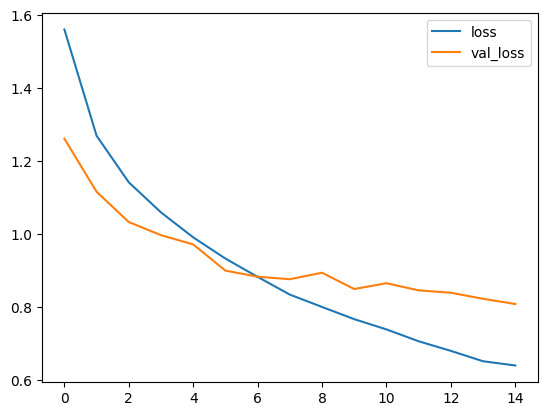
\includegraphics[width=.8\linewidth]{apendices/fig/9_IAA009_1.png}
\caption*{Fonte: O autor (2024).}
\end{figure}

\begin{figure}[H]
\centering
\caption{Acurácia - CNN}
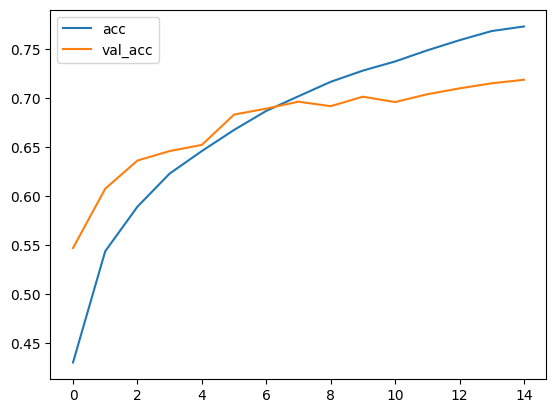
\includegraphics[width=.8\linewidth]{apendices/fig/9_IAA009_2.png}
\caption*{Fonte: O autor (2024).}
\end{figure}


\begin{lstlisting}[language=Python, style=input]
# Efetuar predições na base de teste
# argmax é usado pois a função de ativação da saída é softmax
# argmax pega o neurônio que deu o maior resultado, isto é,
# a maior probabilidade de saída
y_pred = model.predict(x_test).argmax(axis=1)
# Mostrar a matriz de confusão
cm = confusion_matrix(y_test, y_pred)
plot_confusion_matrix(conf_mat=cm, figsize=(7, 7),
show_normed=True)
\end{lstlisting}

\begin{figure}[H]
\centering
\caption{Matriz de confusão - CNN}
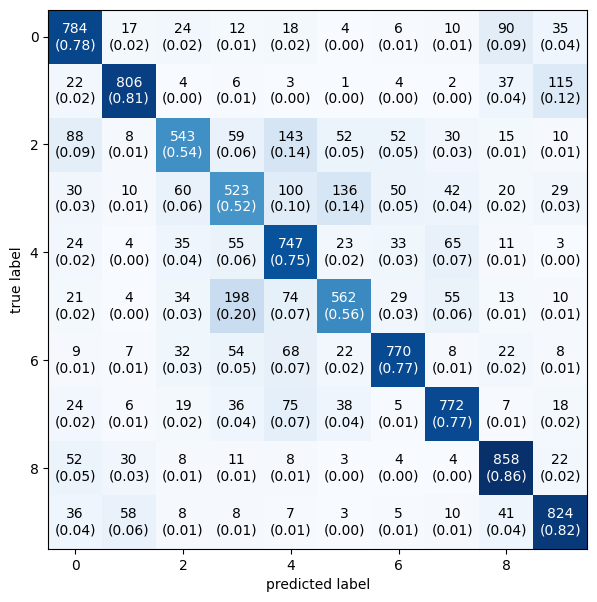
\includegraphics[width=.8\linewidth]{apendices/fig/9_IAA009_3.png}
\caption*{Fonte: O autor (2024).}
\end{figure}

\begin{lstlisting}[language=Python, style=input]
# Mostrar algumas classificações erradas
labels= ["airplane", "automobile", "bird", "cat", "deer", "dog",
"frog", "horse", "ship", "truck"]
misclassified = np.where(y_pred != y_test)[0]
i = np.random.choice(misclassified)
plt.imshow(x_test[i], cmap="gray")
plt.title("True label: %s Predicted: %s" % (labels[y_test[i]],
labels[y_pred[i]]))
\end{lstlisting}

\begin{figure}[H]
\centering
\caption{Classificação errada - CNN}
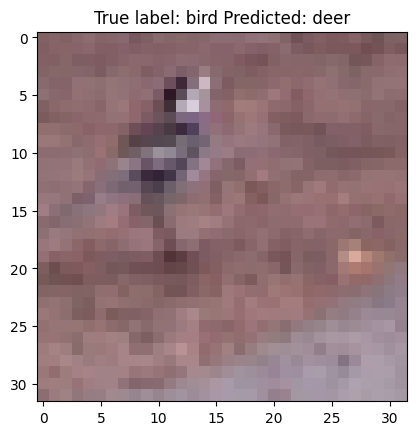
\includegraphics[width=.8\linewidth]{apendices/fig/9_IAA009_4.png}
\caption*{Fonte: O autor (2024).}
\end{figure}

\begin{adjustwidth}{1em}{}
\textbf{2 Detector de SPAM (RNN)}
\end{adjustwidth}
\begin{lstlisting}[language=Python, style=input]
# Importação das Bibliotecas
import tensorflow as tf
import numpy as np
import matplotlib.pyplot as plt
import pandas as pd
from sklearn.model_selection import train_test_split
from tensorflow.keras.layers import Input, Embedding, LSTM, Dense
from tensorflow.keras.layers import GlobalMaxPooling1D
from tensorflow.keras.models import Model
from tensorflow.keras.preprocessing.sequence import pad_sequences
from tensorflow.keras.preprocessing.text import Tokenizer

# carrega e arruma a base
!wget http://www.razer.net.br/datasets/spam.csv
# !wget https://www.kaggle.com/datasets/uciml/sms-spam-collection-dataset
df = pd.read_csv("spam.csv", encoding="ISO-8859-1")
df.head()
df = df.drop(["Unnamed: 2", "Unnamed: 3", "Unnamed: 4"], axis=1)
df.columns = ["labels", "data"]
df["b_labels"] = df["labels"].map({ "ham": 0, "spam": 1})
y = df["b_labels"].values

# Separa a base em treino e teste
x_train, x_test, y_train, y_test = train_test_split(df["data"], y,
test_size=0.33)

# Número máximo de palavras para considerar
# São consideradas as mais frequentes, as demais são
#   ignoradas
num_words = 20000
tokenizer = Tokenizer(num_words=num_words)
tokenizer.fit_on_texts(x_train)
sequences_train = tokenizer.texts_to_sequences(x_train)
sequences_test = tokenizer.texts_to_sequences(x_test)
word2index = tokenizer.word_index
V = len(word2index)

# Acerta o tamanho das sequências (padding)
data_train = pad_sequences(sequences_train) # usa o tamanho da maior seq.
T = data_train.shape[1] # tamanho da sequência
data_test = pad_sequences(sequences_test, maxlen=T)
print("%s tokens" % V)
print("data_train.shape: ", data_train.shape)
print("data_test.shape: ", data_test.shape)
\end{lstlisting}

\begin{tcolorbox}[myoutputstyle]
7201 tokens\\
data\_train.shape:  (3733, 189)\\
data\_test.shape:  (1839, 189)
\end{tcolorbox}


\begin{lstlisting}[language=Python, style=input]
# Define o modelo
D = 20   # tamanho do embedding, hiperparâmetro que pode ser escolhido
M = 5    # tamanho do hidden state, quantidade de unidades LSTM
i = Input(shape=(T,)) # Entra uma frase inteira
x = Embedding(V+1, D)(i)
x = LSTM(M)(x)
x = Dense(1, activation="sigmoid")(x) # Sigmoide pois só tem 2 valores
model = Model(i, x)
model.summary()
\end{lstlisting}

\begin{tcolorbox}[myoutputstyle]
Model: "functional"
\begin{table}[H]
%\centering
\begin{tabular}{|l|c|r|}
\hline
\textbf{Layer (type)} & \textbf{Output Shape} & \textbf{Param \#} \\ \hline
input\_layer (InputLayer) & (None, 189) & 0 \\ \hline
embedding (Embedding) & (None, 189, 20) & 143,980 \\ \hline
lstm (LSTM) & (None, 5) & 520 \\ \hline
dense (Dense) & (None, 1) & 6 \\ \hline
\end{tabular}
%\caption{Model summary}
\end{table}
 Total params: 144,506 (564.48 KB)\\
 Trainable params: 144,506 (564.48 KB)\\
 Non-trainable params: 0 (0.00 B)
\end{tcolorbox}

\begin{lstlisting}[language=Python, style=input]
# Compila e treina o modelo
model.compile(loss="binary_crossentropy", optimizer="adam",
metrics=["accuracy"])
epochs = 5
r = model.fit(data_train, y_train, epochs=epochs, validation_data=(data_test,
y_test))

# Plota função de perda e acurácia
plt.plot(r.history["loss"], label="loss")
plt.plot(r.history["val_loss"], label="val_loss")
plt.xlabel("Epocas")
plt.ylabel("loss")
plt.xticks(np.arange(0, epochs, step=1), labels=range(1, epochs+1))
plt.legend()
plt.show()
plt.plot(r.history["accuracy"], label="accuracy")
plt.plot(r.history["val_accuracy"], label="val_accuracy")
plt.xlabel("Epocas")
plt.ylabel("Acurácia")
plt.xticks(np.arange(0, epochs, step=1), labels=range(1, epochs+1))
plt.legend()
plt.show()
\end{lstlisting}


\begin{figure}[H]
\centering
\caption{Função de perda - RNN}
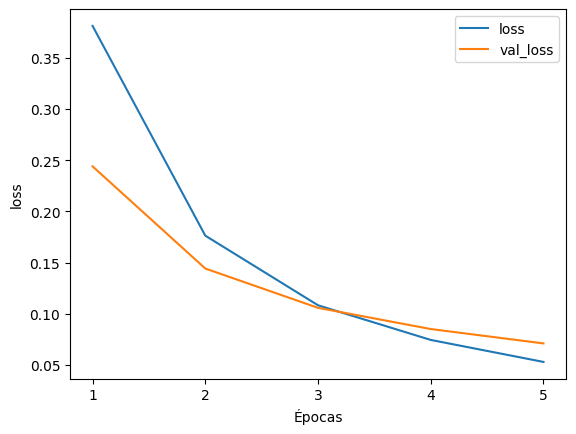
\includegraphics[width=.8\linewidth]{apendices/fig/9_IAA009_5.png}
\caption*{Fonte: O autor (2024).}
\end{figure}

\begin{figure}[H]
\centering
\caption{Acurácia - RNN}
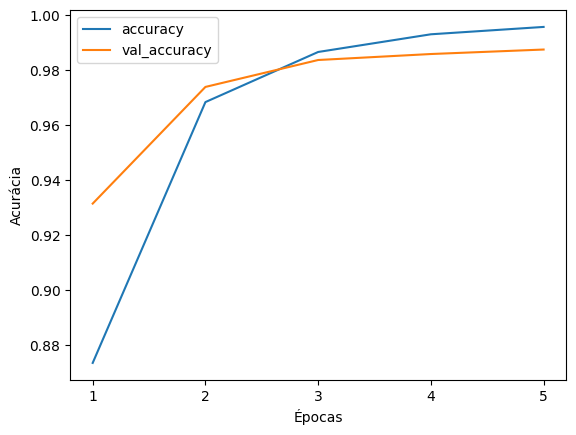
\includegraphics[width=.8\linewidth]{apendices/fig/9_IAA009_6.png}
\caption*{Fonte: O autor (2024).}
\end{figure}

\begin{lstlisting}[language=Python, style=input]
# Efetua a predição de um texto novo
#texto = "Hi, my name is Razer and want to tell you something."
texto = "Is your car dirty? Discover our new product. Free for all. Click the link."
seq_texto = tokenizer.texts_to_sequences([texto]) # Tokeniza
data_texto = pad_sequences(seq_texto, maxlen=T)   # Padding
pred = model.predict(data_texto) # Predição
print(pred)
print ("SPAM" if pred >= 0.5 else "OK")
\end{lstlisting}

\begin{tcolorbox}[myoutputstyle]
[[0.7768526]]\\
SPAM
\end{tcolorbox}


%%%%%%%%%%%%%%%%%%%%%%%%%%%%%%%%%%%%%%%%%%%%%%%%%%%%%%%%%%%%%%%%%%%%%%%%%%%%%%%%%%%%%%%%%%%
\begin{adjustwidth}{1em}{}
\textbf{3 Gerador de Dígitos Fake (GAN)}
\end{adjustwidth}

\begin{lstlisting}[language=Python, style=input]
!pip install imageio
!pip install git+https://github.com/tensorflow/docs

# Importações
import tensorflow as tf
import glob
import imageio
import matplotlib.pyplot as plt
import numpy as np
import os
import PIL
from tensorflow.keras import layers
import time
from IPython import display

# Carregar a base de dados
(train_images, train_labels), (_, _) = tf.keras.datasets.mnist.load_data()
# Normalização
train_images = train_images.reshape(train_images.shape[0], 28, 28, 1).astype('float32')
train_images = (train_images - 127.5) / 127.5  # Normaliza entre [-1, 1]
# Gera o banco em partes e randomiza
BUFFER_SIZE = 60000
BATCH_SIZE = 256
# Cria o dataset (from_tensor_slices)
# Randomiza (shuffle)
# Combina elementos consecutivos em lotes (batch)
train_dataset = tf.data.Dataset.from_tensor_slices(train_images).shuffle(BUFFER_SIZE).batch(BATCH_SIZE)

# Cria o GERADOR
def make_generator_model():
  model = tf.keras.Sequential()
  model.add(layers.Dense(7*7*256, use_bias=False,input_shape=(100,)))
  model.add(layers.BatchNormalization())
  model.add(layers.LeakyReLU())

  model.add(layers.Reshape((7, 7, 256)))
  assert model.output_shape == (None, 7, 7, 256)

  # Note: None is the batch size
  model.add(layers.Conv2DTranspose(128, (5, 5), strides=(1, 1), padding='same', use_bias=False))
  assert model.output_shape == (None, 7, 7, 128)

  model.add(layers.BatchNormalization())
  model.add(layers.LeakyReLU())

  model.add(layers.Conv2DTranspose(64, (5, 5), strides=(2, 2), padding='same', use_bias=False))
  assert model.output_shape == (None, 14, 14, 64)
  model.add(layers.BatchNormalization())
  model.add(layers.LeakyReLU())

  model.add(layers.Conv2DTranspose(1, (5, 5), strides=(2, 2), padding='same', use_bias=False, activation='tanh'))
  assert model.output_shape == (None, 28, 28, 1)
  return model

# Teste do GERADOR, ainda não treinado
generator = make_generator_model()

noise = tf.random.normal([1, 100])
generated_image = generator(noise, training=False)

plt.imshow(generated_image[0, :, :, 0], cmap='gray')
\end{lstlisting}

\begin{figure}[H]
\centering
\caption{Teste gerador - GAN}
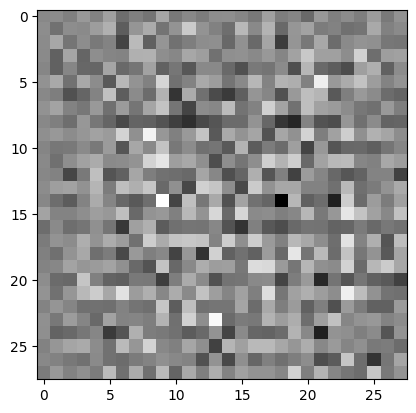
\includegraphics[width=.7\linewidth]{apendices/fig/9_IAA009_7.png}
\caption*{Fonte: O autor (2024).}
\end{figure}


\begin{lstlisting}[language=Python, style=input]
# Cria o DISCRIMINADOR
def make_discriminator_model():
  model = tf.keras.Sequential()
  model.add(layers.Conv2D(64, (5, 5), strides=(2, 2), padding='same', input_shape=[28, 28, 1]))
  model.add(layers.LeakyReLU())
  model.add(layers.Dropout(0.3))

  model.add(layers.Conv2D(128, (5, 5), strides=(2, 2), padding='same'))
  model.add(layers.LeakyReLU())
  model.add(layers.Dropout(0.3))

  model.add(layers.Flatten())
  model.add(layers.Dense(1))
  return model

# Teste do DISCRIMINADOR, ainda não treinado
discriminator = make_discriminator_model()
decision = discriminator(generated_image)
#print (decision)

# Define as funções de perda
cross_entropy = tf.keras.losses.BinaryCrossentropy(from_logits=True)

# Perda do DISCRIMINADOR
def discriminator_loss(real_output, fake_output):
  real_loss = cross_entropy(tf.ones_like(real_output), real_output)
  fake_loss = cross_entropy(tf.zeros_like(fake_output), fake_output)
  total_loss = real_loss + fake_loss
  return total_loss

# Perda do GERADOR
def generator_loss(fake_output):
  return cross_entropy(tf.ones_like(fake_output), fake_output)

# Cria os otimizadores para o gerador e discriminador
generator_optimizer = tf.keras.optimizers.Adam(1e-4)
discriminator_optimizer = tf.keras.optimizers.Adam(1e-4)

# Cria checkpoints para salvar modelos ao longo do tempo
# Uteis em tarefas longas, para se recuperar de um desligamento
checkpoint_dir = './training_checkpoints'
checkpoint_prefix = os.path.join(checkpoint_dir, "ckpt")
checkpoint = tf.train.Checkpoint(generator_optimizer=generator_optimizer,
                                 discriminator_optimizer=discriminator_optimizer,
                                 generator=generator,
                                 discriminator=discriminator)

                             # Configura o Loop de treinamento
EPOCHS = 100
noise_dim = 100
num_examples_to_generate = 16
# You will reuse this seed overtime (so it's easier)
# to visualize progress in the animated GIF)
seed = tf.random.normal([num_examples_to_generate, noise_dim])

def f(x, y):
  return 3*x**2 + 2*x*y

x, y = tf.Variable(5.), tf.Variable(3.)
with tf.GradientTape() as tape:
  z = f(x, y)
gradients = tape.gradient(z, [x, y])
print(gradients)

# Função que faz um passo de treinamento
# E uma tf.function, que compila essa funcao
@tf.function
def train_step(images):
  noise = tf.random.normal([BATCH_SIZE, noise_dim])

  with tf.GradientTape() as gen_tape, tf.GradientTape() as disc_tape:
    generated_images = generator(noise, training=True)

    real_output = discriminator(images, training=True)
    fake_output = discriminator(generated_images, training=True)

    gen_loss = generator_loss(fake_output)
    disc_loss = discriminator_loss(real_output, fake_output)

  gradients_of_generator = gen_tape.gradient(gen_loss, generator.trainable_variables)
  gradients_of_discriminator = disc_tape.gradient(disc_loss, discriminator.trainable_variables)

  generator_optimizer.apply_gradients(zip(gradients_of_generator, generator.trainable_variables))
  discriminator_optimizer.apply_gradients(zip(gradients_of_discriminator, discriminator.trainable_variables))

# Treinamento completo/laço
def train(dataset, epochs):
  for epoch in range(epochs):
    start = time.time()

    for image_batch in dataset:
      train_step(image_batch)

    # Produce images for the GIF as you go
    display.clear_output(wait=True)
    generate_and_save_images(generator, epoch + 1, seed)

    # Save the model every 15 epochs
    if (epoch + 1) % 15 == 0:
      checkpoint.save(file_prefix = checkpoint_prefix)

    print ('Time for epoch {} is {} sec'.format(epoch + 1, time.time() - start))

  # Generate after the final epoch
  display.clear_output(wait=True)
  generate_and_save_images(generator, epochs, seed)

def generate_and_save_images(model, epoch, test_input):
  # Notice `training` is set to False.
  # This is so all layers run in inference mode (batchnorm).
  predictions = model(test_input, training=False)
  fig = plt.figure(figsize=(4, 4))

  for i in range(predictions.shape[0]):
    plt.subplot(4, 4, i+1)
    plt.imshow(predictions[i, :, :, 0] * 127.5 + 127.5, cmap='gray')
    plt.axis('off')

  plt.savefig('image_at_epoch_{:04d}.png'.format(epoch))
  plt.show()

train(train_dataset, EPOCHS)
checkpoint.restore(tf.train.latest_checkpoint(checkpoint_dir))
\end{lstlisting}

\begin{figure}[H]
\centering
\caption{Imagem na ultima epoca - GAN}
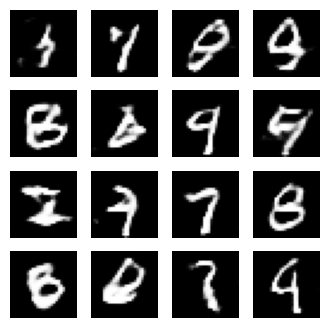
\includegraphics[width=.6\linewidth]{apendices/fig/9_IAA009_8.png}
\caption*{Fonte: O autor (2024).}
\end{figure}

%%%%%%%%%%%%%%%%%%%%%%%%%%%%%%%%%%%%%%%%%%%%%%%%%%%%%%%%%%%%%%%%%%%%%%%%%%%%%%%%%%%%%%%%%%%
\begin{adjustwidth}{1em}{}
\textbf{4 Tradutor de Textos (Transformer)}
\end{adjustwidth}


\begin{lstlisting}[language=Python, style=input]
# Instalação e importação
!pip uninstall -y tensorflow
!pip uninstall -y tf-keras
!pip install tf-keras==2.15.1
!pip install tensorflow==2.15.0 #--use-deprecated=legacy-resolver
!pip install tensorflow_datasets
!pip install -U tensorflow-text==2.15.0
pip install matplotlib

import collections
import logging
import os
import pathlib
import re
import string
import sys
import time

import numpy as np
import matplotlib.pyplot as plt

import tensorflow_datasets as tfds
import tensorflow_text as text
import tensorflow as tf

logging.getLogger('tensorflow').setLevel(logging.ERROR)  # suppress warnings

# Carregar a base de dados
examples, metadata = tfds.load('ted_hrlr_translate/pt_to_en', with_info=True, as_supervised=True)
train_examples, val_examples = examples['train'], examples['validation']

# Verificar o dataset
for pt_examples, en_examples in train_examples.batch(3).take(1):
  for pt in pt_examples.numpy():
    print(pt.decode('utf-8'))
  print()

  for en in en_examples.numpy():
    print(en.decode('utf-8'))
\end{lstlisting}

\begin{tcolorbox}[myoutputstyle]
e quando melhoramos a procura , tiramos a única vantagem da impressão , que é a serendipidade .\\
mas e se estes fatores fossem ativos ?\\
mas eles não tinham a curiosidade de me testar .\\
\\
and when you improve searchability , you actually take away the one advantage of print , which is serendipity .\\
but what if it were active ?\\
but they did n't test for curiosity .
\end{tcolorbox}


\begin{lstlisting}[language=Python, style=input]
# Tokenização e Destokenização do texto
model_name = "ted_hrlr_translate_pt_en_converter"

tf.keras.utils.get_file(f"{model_name}.zip", f"https://storage.googleapis.com/download.tensorflow.org/models/{model_name}.zip", cache_dir='.', cache_subdir='', extract=True)
# Tem 2 tokenizers: um pt outro em en tokenizers.en tokeniza e detokeniza
tokenizers = tf.saved_model.load(model_name)

# PIPELINE DE ENTRADA
# Codificar/tokenizar lotes de texto puro
def tokenize_pairs(pt, en):
  pt = tokenizers.pt.tokenize(pt)
  # Converte ragged (irregular, tam variável) para dense
  # Faz padding com zeros.
  pt = pt.to_tensor()

  en = tokenizers.en.tokenize(en)
  # ragged -> dense
  en = en.to_tensor()
  return pt, en

# Pipeline simpes: processa, embaralha, agrupa os dados, prefetch
# Datasets de entrada terminam com prefetch
BUFFER_SIZE = 20000
BATCH_SIZE = 64

def make_batches(ds):
  return (
    ds
    .cache()
    .shuffle(BUFFER_SIZE)
    .batch(BATCH_SIZE)
    .map(tokenize_pairs, num_parallel_calls=tf.data.AUTOTUNE)
    .prefetch(tf.data.AUTOTUNE)
  )

train_batches = make_batches(train_examples)
val_batches = make_batches(val_examples)

# CODIFICACAO POSICIONAL
def get_angles(pos, i, d_model):
  angle_rates = 1 / np.power(10000, (2 * (i//2)) / np.float32(d_model))
  return pos * angle_rates

def positional_encoding(position, d_model):
  angle_rads = get_angles(np.arange(position)[:, np.newaxis],np.arange(d_model)[np.newaxis, :],d_model)
  # sin em índices pares no array; 2i
  angle_rads[:, 0::2] = np.sin(angle_rads[:, 0::2])
  # cos em índices ímpares no array; 2i+1
  angle_rads[:, 1::2] = np.cos(angle_rads[:, 1::2])
  # newaxis, aumenta a dimensão [] -> [ [] ]

  pos_encoding = angle_rads[np.newaxis, ...]
  return tf.cast(pos_encoding, dtype=tf.float32)

# CODIFICACAO POSICIONAL
n, d = 2048, 512
pos_encoding = positional_encoding(n, d)
print(pos_encoding.shape)
pos_encoding = pos_encoding[0]

# Arrumar as dimensões
pos_encoding = tf.reshape(pos_encoding, (n, d//2, 2))
pos_encoding = tf.transpose(pos_encoding, (2, 1, 0))
pos_encoding = tf.reshape(pos_encoding, (d, n))

plt.pcolormesh(pos_encoding, cmap='RdBu')
plt.ylabel('Depth')
plt.xlabel('Position')
plt.colorbar()
plt.show()
\end{lstlisting}


\begin{figure}[H]
\centering
\caption{Colomesh - Transformer}
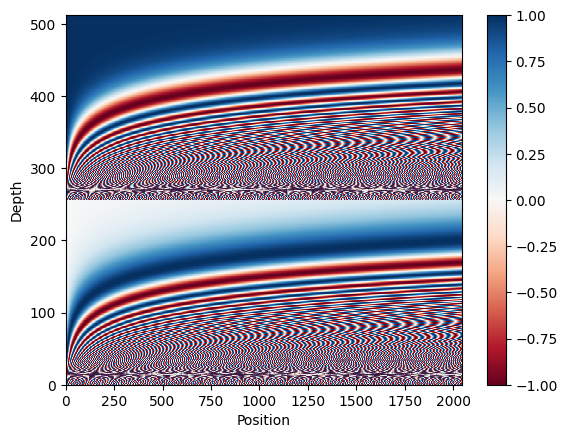
\includegraphics[width=.7\linewidth]{apendices/fig/9_IAA009_9.png}
\caption*{Fonte: O autor (2024).}
\end{figure}


\begin{lstlisting}[language=Python, style=input]
# Cria uma máscara de 0 e 1, 0 para quando há valor e 1 quando não há
def create_padding_mask(seq):
  seq = tf.cast(tf.math.equal(seq, 0), tf.float32)
  # add extra dimensions to add the padding
  # to the attention logits.
  return seq[:, tf.newaxis, tf.newaxis, :]  # (batch_size, 1, 1, seq_l)

# Máscara futura, usada no decoder
def create_look_ahead_mask(size):
  # zera o triângulo inferior
  mask = 1 - tf.linalg.band_part(tf.ones((size, size)), -1, 0)
  return mask # (seq_len, seq_len)

# Função de Atenção
def scaled_dot_product_attention(q, k, v, mask):
  # Q K^T
  matmul_qk = tf.matmul(q, k, transpose_b=True)  # (..., seq_len_q, seq_len_k)
  # converte matmul_qk para float32
  dk = tf.cast(tf.shape(k)[-1], tf.float32)

  # divide por sqrt(d_k)
  scaled_attention_logits = matmul_qk / tf.math.sqrt(dk)

  # Soma a máscara, e os valores faltantes serão um número próximo a -inf
  if mask is not None:
    scaled_attention_logits += (mask * -1e9)

  # softmax normaliza os dados, soman 1. // (..., seq_len_q, seq_len_k)
  attention_weights = tf.nn.softmax(scaled_attention_logits, axis=-1)
  output = tf.matmul(attention_weights, v)  # (..., seq_len_q, depth_v)
  return output, attention_weights

# Atenção Multi-cabeças
class MultiHeadAttention(tf.keras.layers.Layer):
  def __init__(self, d_model, num_heads):
    super(MultiHeadAttention, self).__init__()
    self.num_heads = num_heads
    self.d_model = d_model
    assert d_model % self.num_heads == 0
    self.depth = d_model // self.num_heads

    self.wq = tf.keras.layers.Dense(d_model)
    self.wk = tf.keras.layers.Dense(d_model)
    self.wv = tf.keras.layers.Dense(d_model)

    self.dense = tf.keras.layers.Dense(d_model)

  def split_heads(self, x, batch_size):
    #"Separa a última dimensão em (num_heads, depth).Transpõe o resultado para o shape (batch_size, num_heads, seq_len, depth)"
    x = tf.reshape(x, (batch_size, -1, self.num_heads, self.depth))
    return tf.transpose(x, perm=[0, 2, 1, 3])

  def call(self, v, k, q, mask):
    batch_size = tf.shape(q)[0]

    q = self.wq(q)  # (batch_size, seq_len, d_model)
    k = self.wk(k)  # (batch_size, seq_len, d_model)
    v = self.wv(v)  # (batch_size, seq_len, d_model)

    q = self.split_heads(q, batch_size)  # (batch_size, num_heads, seq_len_q, depth)
    k = self.split_heads(k, batch_size)  # (batch_size, num_heads, seq_len_k, depth)
    v = self.split_heads(v, batch_size)  # (batch_size, num_heads, seq_len_v, depth)

    # Calcula a atenção para cada cabeça (de forma matricial)
    # scaled_attention.shape == (batch_size, num_heads, seq_len_q, depth)
    # attention_weights.shape == (batch_size, num_heads, seq_len_q, seq_len_k)
    scaled_attention, attention_weights = scaled_dot_product_attention(q, k, v, mask)

    # Troca a dimensão 2 com 1, para acertar o num_heads# (batch_size, seq_len_q, num_heads, depth)
    scaled_attention = tf.transpose(scaled_attention, perm=[0, 2, 1, 3])
    # Concatena os valores em: (batch_size, seq_len_q, d_model)
    concat_attention = tf.reshape(scaled_attention, (batch_size, -1, self.d_model))
    output = self.dense(concat_attention)  # (batch_size, seq_len_q, d_model)
    return output, attention_weights

def point_wise_feed_forward_network(d_model, dff):
  return tf.keras.Sequential([
    tf.keras.layers.Dense(dff, activation='relu'),  # (batch_size, seq_len, dff)
    tf.keras.layers.Dense(d_model)  # (batch_size, seq_len, d_model)
  ])

class EncoderLayer(tf.keras.layers.Layer):
  def __init__(self, d_model, num_heads, dff, rate=0.1):
    super(EncoderLayer, self).__init__()
    self.mha = MultiHeadAttention(d_model, num_heads)
    self.ffn = point_wise_feed_forward_network(d_model, dff)

    self.layernorm1 = tf.keras.layers.LayerNormalization(epsilon=1e-6)
    self.layernorm2 = tf.keras.layers.LayerNormalization(epsilon=1e-6)

    self.dropout1 = tf.keras.layers.Dropout(rate)
    self.dropout2 = tf.keras.layers.Dropout(rate)

  def call(self, x, training, mask):
    attn_output, _ = self.mha(x, x, x, mask)
    attn_output = self.dropout1(attn_output, training=training)
    out1 = self.layernorm1(x + attn_output)
    ffn_output = self.ffn(out1)
    ffn_output = self.dropout2(ffn_output, training=training)
    out2 = self.layernorm2(out1 + ffn_output)

    return out2

class DecoderLayer(tf.keras.layers.Layer):
  def __init__(self, d_model, num_heads, dff, rate=0.1):
    super(DecoderLayer, self).__init__()

    self.mha1 = MultiHeadAttention(d_model, num_heads)
    self.mha2 = MultiHeadAttention(d_model, num_heads)
    self.ffn = point_wise_feed_forward_network(d_model, dff)

    self.layernorm1 = tf.keras.layers.LayerNormalization(epsilon=1e-6)
    self.layernorm2 = tf.keras.layers.LayerNormalization(epsilon=1e-6)
    self.layernorm3 = tf.keras.layers.LayerNormalization(epsilon=1e-6)

    self.dropout1 = tf.keras.layers.Dropout(rate)
    self.dropout2 = tf.keras.layers.Dropout(rate)
    self.dropout3 = tf.keras.layers.Dropout(rate)

  def call(self, x, enc_output, training, look_ahead_mask, padding_mask):
    # enc_output.shape == (batch_size, input_seq_len, d_model)
    # (batch_size, target_seq_len, d_model)
    attn1, attn_weights_block1 = self.mha1(x, x, x, look_ahead_mask)
    attn1 = self.dropout1(attn1, training=training)
    out1 = self.layernorm1(attn1 + x)

    # (batch_size, target_seq_len, d_model)
    attn2, attn_weights_block2 = self.mha2(enc_output, enc_output, out1, padding_mask)
    attn2 = self.dropout2(attn2, training=training)
    out2 = self.layernorm2(attn2 + out1)  # (batch_size, target_seq_len, d_model)

    ffn_output = self.ffn(out2)  # (batch_size, target_seq_len, d_model)
    ffn_output = self.dropout3(ffn_output, training=training)
    out3 = self.layernorm3(ffn_output + out2)  # (batch_size, target_seq_len, d_model)

    return out3, attn_weights_block1, attn_weights_block2

class Encoder(tf.keras.layers.Layer):
  def __init__(self, num_layers, d_model, num_heads, dff, input_vocab_size, maximum_position_encoding, rate=0.1):
    super(Encoder, self).__init__()
    self.d_model = d_model
    self.num_layers = num_layers
    self.embedding = tf.keras.layers.Embedding(input_vocab_size, d_model)
    self.pos_encoding = positional_encoding(maximum_position_encoding, self.d_model)
    self.enc_layers = [EncoderLayer(d_model, num_heads, dff, rate) for _ in range(num_layers)]
    self.dropout = tf.keras.layers.Dropout(rate)

  def call(self, x, training, mask):
    seq_len = tf.shape(x)[1]
    # adding embedding and position encoding.
    x = self.embedding(x)  # (batch_size, input_seq_len, d_model)
    x *= tf.math.sqrt(tf.cast(self.d_model, tf.float32))
    x += self.pos_encoding[:, :seq_len, :]
    x = self.dropout(x, training=training)
    for i in range(self.num_layers):
      x = self.enc_layers[i](x, training, mask)
    return x # (batch_size, input_seq_len, d_model)

class Decoder(tf.keras.layers.Layer):
  def __init__(self, num_layers, d_model, num_heads, dff, target_vocab_size,
    maximum_position_encoding, rate=0.1):
    super(Decoder, self).__init__()
    self.d_model = d_model
    self.num_layers = num_layers
    self.embedding = tf.keras.layers.Embedding(target_vocab_size, d_model)
    self.pos_encoding = positional_encoding(maximum_position_encoding, d_model)
    self.dec_layers = [DecoderLayer(d_model, num_heads, dff, rate) for _ in range(num_layers)]
    self.dropout = tf.keras.layers.Dropout(rate)

  def call(self, x, enc_output, training, look_ahead_mask, padding_mask):
    seq_len = tf.shape(x)[1]
    attention_weights = {}
    x = self.embedding(x)  # (batch_size, target_seq_len, d_model)
    x *= tf.math.sqrt(tf.cast(self.d_model, tf.float32))
    x += self.pos_encoding[:, :seq_len, :]
    x = self.dropout(x, training=training)
    for i in range(self.num_layers):
      x, block1, block2 = self.dec_layers[i](x, enc_output, training,look_ahead_mask, padding_mask)
      attention_weights[f'decoder_layer{i+1}_block1'] = block1
      attention_weights[f'decoder_layer{i+1}_block2'] = block2
    # x.shape == (batch_size, target_seq_len, d_model)
    return x, attention_weights

class Transformer(tf.keras.Model):
  def __init__(self, num_layers, d_model, num_heads, dff, input_vocab_size, target_vocab_size, pe_input, pe_target, rate=0.1):
    super().__init__()
    self.encoder = Encoder(num_layers, d_model, num_heads, dff, input_vocab_size, pe_input, rate)
    self.decoder = Decoder(num_layers, d_model, num_heads, dff, target_vocab_size, pe_target, rate)
    self.final_layer = tf.keras.layers.Dense(target_vocab_size)

  def call(self, inputs, training):
    # Keras models prefer if you pass all your inputs in the first argument
    inp, tar = inputs

    enc_padding_mask, look_ahead_mask, dec_padding_mask = self.create_masks(inp, tar)
    # (batch_size, inp_seq_len, d_model)
    enc_output = self.encoder(inp, training, enc_padding_mask)
    # dec_output.shape == (batch_size, tar_seq_len, d_model)
    dec_output, attention_weights = self.decoder(tar, enc_output, training, look_ahead_mask, dec_padding_mask)
    # (batch_size, tar_seq_len, target_vocab_size)
    final_output = self.final_layer(dec_output)

    return final_output, attention_weights

  def create_masks(self, inp, tar):
    # Encoder padding mask
    enc_padding_mask = create_padding_mask(inp)
    # Used in the 2nd attention block in the decoder.
    # This padding mask is used to mask the encoder outputs.
    dec_padding_mask = create_padding_mask(inp)
    # Used in the 1st attention block in the decoder.
    # It is used to pad and mask future tokens in the input received by
    # the decoder.
    look_ahead_mask = create_look_ahead_mask(tf.shape(tar)[1])
    dec_target_padding_mask = create_padding_mask(tar)
    look_ahead_mask = tf.maximum(dec_target_padding_mask, look_ahead_mask)
    return enc_padding_mask, look_ahead_mask, dec_padding_mask

# Hiperparâmetros
num_layers = 4
d_model = 128
dff = 512
num_heads = 8
dropout_rate = 0.1

class CustomSchedule(tf.keras.optimizers.schedules.LearningRateSchedule):
  def __init__(self, d_model, warmup_steps=4000):
    super(CustomSchedule, self).__init__()
    self.d_model = d_model
    self.d_model = tf.cast(self.d_model, tf.float32)
    self.warmup_steps = warmup_steps

  def __call__(self, step):
    step = tf.cast(step, tf.float32) # Adicionado para evitar ERRO
    arg1 = tf.math.rsqrt(step)
    arg2 = step * (self.warmup_steps ** -1.5)
    return tf.math.rsqrt(self.d_model) * tf.math.minimum(arg1, arg2)

learning_rate = CustomSchedule(d_model)
optimizer = tf.keras.optimizers.Adam(learning_rate, beta_1=0.9, beta_2=0.98, epsilon=1e-9)

loss_object = tf.keras.losses.SparseCategoricalCrossentropy(from_logits=True, reduction='none')

def loss_function(real, pred):
  mask = tf.math.logical_not(tf.math.equal(real, 0))
  loss_ = loss_object(real, pred)
  mask = tf.cast(mask, dtype=loss_.dtype)
  loss_ *= mask
  return tf.reduce_sum(loss_)/tf.reduce_sum(mask)

def accuracy_function(real, pred):
  accuracies = tf.equal(real, tf.argmax(pred, axis=2))
  mask = tf.math.logical_not(tf.math.equal(real, 0))
  accuracies = tf.math.logical_and(mask, accuracies)
  accuracies = tf.cast(accuracies, dtype=tf.float32)
  mask = tf.cast(mask, dtype=tf.float32)
  return tf.reduce_sum(accuracies)/tf.reduce_sum(mask)

train_loss = tf.keras.metrics.Mean(name='train_loss')
train_accuracy = tf.keras.metrics.Mean(name='train_accuracy')

transformer = Transformer(
  num_layers=num_layers,
  d_model=d_model,
  num_heads=num_heads,
  dff=dff,
  input_vocab_size=tokenizers.pt.get_vocab_size().numpy(),
  target_vocab_size=tokenizers.en.get_vocab_size().numpy(),
  pe_input=1000,
  pe_target=1000,
  rate=dropout_rate)

# Checkpoint
checkpoint_path = "./checkpoints/train"

ckpt = tf.train.Checkpoint(transformer=transformer, optimizer=optimizer)

ckpt_manager = tf.train.CheckpointManager(ckpt, checkpoint_path, max_to_keep=5)

# if a checkpoint exists, restore the latest checkpoint.
if ckpt_manager.latest_checkpoint:
  ckpt.restore(ckpt_manager.latest_checkpoint)
  print('Latest checkpoint restored!!')

EPOCHS = 20

train_step_signature = [
  tf.TensorSpec(shape=(None, None), dtype=tf.int64),
  tf.TensorSpec(shape=(None, None), dtype=tf.int64),
]
@tf.function(input_signature=train_step_signature)
def train_step(inp, tar):
  tar_inp = tar[:, :-1]
  tar_real = tar[:, 1:]
  with tf.GradientTape() as tape:
    predictions, _ = transformer([inp, tar_inp], training = True)
    loss = loss_function(tar_real, predictions)

  gradients = tape.gradient(loss, transformer.trainable_variables)
  optimizer.apply_gradients(zip(gradients, transformer.trainable_variables))

  train_loss(loss)
  train_accuracy(accuracy_function(tar_real, predictions))

for epoch in range(EPOCHS):
  start = time.time()
  train_loss.reset_state()
  train_accuracy.reset_state()

  # inp -> portuguese, tar -> english
  for (batch, (inp, tar)) in enumerate(train_batches):
    train_step(inp, tar)
    if batch % 50 == 0:
      print(f'Epoch {epoch + 1} Batch {batch} Loss {train_loss.result():.4f} Accuracy{train_accuracy.result():.4f}')

  if (epoch + 1) % 5 == 0:
    ckpt_save_path = ckpt_manager.save()
    print(f'Saving checkpoint for epoch {epoch+1} at {ckpt_save_path}')

  print(f'Epoch {epoch + 1} Loss {train_loss.result():.4f} Accuracy{train_accuracy.result():.4f}')
  print(f'Time taken for 1 epoch: {time.time() - start:.2f} secs\n')
\end{lstlisting}

\begin{tcolorbox}[myoutputstyle]
...\\
Epoch 20 Batch 0 Loss 1.4398 Accuracy0.6776\\
Epoch 20 Batch 50 Loss 1.4214 Accuracy0.6838\\
Epoch 20 Batch 100 Loss 1.4334 Accuracy0.6820\\
Epoch 20 Batch 150 Loss 1.4287 Accuracy0.6833\\
Epoch 20 Batch 200 Loss 1.4364 Accuracy0.6820\\
Epoch 20 Batch 250 Loss 1.4398 Accuracy0.6815\\
Epoch 20 Batch 300 Loss 1.4402 Accuracy0.6813\\
Epoch 20 Batch 350 Loss 1.4458 Accuracy0.6804\\
Epoch 20 Batch 400 Loss 1.4458 Accuracy0.6805\\
Epoch 20 Batch 450 Loss 1.4450 Accuracy0.6804\\
Epoch 20 Batch 500 Loss 1.4463 Accuracy0.6801\\
Epoch 20 Batch 550 Loss 1.4490 Accuracy0.6795\\
Epoch 20 Batch 600 Loss 1.4511 Accuracy0.6793\\
Epoch 20 Batch 650 Loss 1.4533 Accuracy0.6788\\
Epoch 20 Batch 700 Loss 1.4567 Accuracy0.6782\\
Epoch 20 Batch 750 Loss 1.4590 Accuracy0.6778\\
Epoch 20 Batch 800 Loss 1.4610 Accuracy0.6775\\
Saving checkpoint for epoch 20 at ./checkpoints/train/ckpt-4\\
Epoch 20 Loss 1.4617 Accuracy0.6774\\
Time taken for 1 epoch: 95.57 secs
\end{tcolorbox}


\begin{lstlisting}[language=Python, style=input]
class Translator(tf.Module):
  def __init__(self, tokenizers, transformer):
    self.tokenizers = tokenizers
    self.transformer = transformer
  def __call__(self, sentence, max_length=20):
    # input sentence is portuguese, hence adding the start and end token
    assert isinstance(sentence, tf.Tensor)
    if len(sentence.shape) == 0:
      sentence = sentence[tf.newaxis]
    sentence = self.tokenizers.pt.tokenize(sentence).to_tensor()
    encoder_input = sentence
    # as the target is english, the first token to the transformer should be the
    # english start token.
    start_end = self.tokenizers.en.tokenize([''])[0]
    start = start_end[0][tf.newaxis]
    end = start_end[1][tf.newaxis]
    output_array = tf.TensorArray(dtype=tf.int64, size=0, dynamic_size=True)
    output_array = output_array.write(0, start)
    for i in tf.range(max_length):
      output = tf.transpose(output_array.stack())
      predictions, _ = self.transformer([encoder_input, output], training=False)
      predictions = predictions[:, -1:, :]  # (batch_size, 1, vocab_size)
      predicted_id = tf.argmax(predictions, axis=-1)
      output_array = output_array.write(i+1, predicted_id[0])
      if predicted_id == end:
        break

    output = tf.transpose(output_array.stack())
    # output.shape (1, tokens)
    text = tokenizers.en.detokenize(output)[0]
    tokens = tokenizers.en.lookup(output)[0]
    _, attention_weights = self.transformer([encoder_input, output[:,:-1]], training=False)
    return text, tokens, attention_weights

translator = Translator(tokenizers, transformer)

sentence = "Eu li sobre triceratops na enciclopédia."

translated_text, translated_tokens, attention_weights = translator(tf.constant(sentence))

print(f'{"Prediction":15s}: {translated_text}')
\end{lstlisting}

\begin{tcolorbox}[myoutputstyle]
Prediction     : b'i read about tribucis in egypt .'
\end{tcolorbox}
\label{ap:ap10}
\chapter{Big data}
\section*{\textbf{A - ENUNCIADO}}

\textcolor{black}{Enviar um arquivo PDF contendo uma descrição breve (2 páginas) sobre a implementação de uma aplicação
ou estudo de caso envolvendo Big Data e suas ferramentas (NoSQL e NewSQL). Caracterize os dados e Vs envolvidos, além
da modelagem necessária dependendo dos modelos de dados empregados.}

%%%%%%%%%%%%%%%%%%%%%%%%%%%%%%%%%%%%%%%%%%%%%%%%%%%%%%%%%%%%%%%%%%%%%%%%%%%%%%%%%%%%%%%%%%%%%
\section*{\textbf{B - RESOLUÇÃO}}
\lipsum[30]
\label{ap:ap11}
\chapter{Visão computacional}
\section*{\textbf{A - ENUNCIADO}}

\subsection{Extração de Características }

\textcolor{black}{Os bancos de imagens fornecidos são conjuntos de imagens de 250x250 pixels de imuno-histoquímica
(biópsia) de câncer de mama. No total são 4 classes (0, 1+, 2+ e 3+) que estão divididas em diretórios.  O objetivo é
classificar as imagens nas categorias correspondentes. Uma base de imagens será utilizada para o treinamento e outra
para o teste do treino.}\textcolor{black}{ }

\textcolor{black}{As imagens fornecidas são recortes de uma imagem maior do tipo WSI }\textit{\textcolor{black}{(Whole
Slide Imaging}}\textcolor{black}{) disponibilizada pela Universidade de Warwick
(}\underline{\href{https://pubmed.ncbi.nlm.nih.gov/28771788/}{\textcolor{black}{link}}}\textcolor{black}{)}\textit{\textcolor{black}{.}}\textcolor{black}{ A nomenclatura das imagens
segue o padrão XX\_HER\_YYYY.png, onde XX é o número do paciente e YYYY é o número da imagem recortada. Separe a base
de treino em 80\% para treino e 20\% para validação. }\textbf{\textcolor{black}{Separe por pacientes (XX), não utilize
a separação randômica! Pois, imagens do mesmo paciente não podem estar na base de treino e de validação, pois isso pode
gerar um viés.}}\textcolor{black}{ No caso da CNN VGG16 remova a última camada de classificação e armazene os valores
da penúltima camada como um vetor de características. Após o treinamento, os modelos treinados devem ser validados na
base de teste.}\textcolor{black}{ }

\textcolor{black}{ }

%\textcolor{black}{Tarefas:}\textcolor{black}{ }
\subsubsection*{Tarefas:}

\begin{enumerate}[series=listWWNumxxiv,label=\alph*),ref=\alph*]
\item \textcolor{black}{Carregue a base de dados de }\textbf{\textcolor{black}{Treino.}}\textcolor{black}{ }
\item \textcolor{black}{Crie partições contendo 80\% para treino e 20\% para validação (atenção aos
pacientes).}\textcolor{black}{ }
\item \textcolor{black}{Extraia características utilizando LBP e a CNN VGG16 (gerando um csv para cada
extrator).}\textcolor{black}{ }
\item \textcolor{black}{Treine modelos Random Forest, SVM e RNA para predição dos dados extraídos.}\textcolor{black}{ }
\item \textcolor{black}{Carregue a base de }\textbf{\textcolor{black}{Teste}}\textcolor{black}{ e execute a tarefa 3
nesta base.}\textcolor{black}{ }
\item \textcolor{black}{Aplique os modelos treinados nos dados de treino}\textcolor{black}{ }
\item \textcolor{black}{Calcule as métricas de Sensibilidade, Especificidade e F1-Score com base em suas matrizes de
confusão.}\textcolor{black}{ }
\item \textcolor{black}{Indique qual modelo dá o melhor o resultado e a métrica utilizada}\textcolor{black}{ }
\end{enumerate}
\textcolor{black}{ }

\subsection{Redes Neurais}

\textcolor{black}{Utilize as duas bases do exercício anterior para treinar as Redes Neurais Convolucionais VGG16 e a
Resnet50. Utilize os pesos pré-treinados (}\textit{\textcolor{black}{Transfer Learning}}\textcolor{black}{), refaça as
camadas }\textit{\textcolor{black}{Fully Connected}}\textcolor{black}{ para o problema de 4 classes. Compare os treinos
de 15 épocas com e sem }\textit{\textcolor{black}{Data Augmentation}}\textcolor{black}{. Tanto a VGG16 quanto a
Resnet50 têm como camada de entrada uma imagem 224x224x3, ou seja, uma imagem de 224x224 pixels coloridos (3 canais de
cores). Portanto, será necessário fazer uma transformação de 250x250x3 para 224x224x3. Ao fazer o
}\textit{\textcolor{black}{Data Augmentation }}\textbf{\textit{\textcolor{black}{
}}}\textbf{\textcolor{black}{ cuidado }}\textcolor{black}{ para não alterar demais as cores das imagens e atrapalhar na
classificação.}\textcolor{black}{ }

\textcolor{black}{ }

%\textcolor{black}{Tarefas:}\textcolor{black}{ }
\subsubsection*{Tarefas:}

\begin{enumerate}[series=listWWNumxxv,label=\alph*),ref=\alph*]
\item \textcolor{black}{Utilize a base de dados de }\textbf{\textcolor{black}{Treino}}\textcolor{black}{ já separadas em
treino e validação do exercício anterior}\textcolor{black}{ }
\item \textcolor{black}{Treine modelos VGG16 e Resnet50 adaptadas com e sem }\textit{\textcolor{black}{Data
Augmentation}}\textcolor{black}{ }
\item \textcolor{black}{Aplique os modelos treinados nas imagens da base de
}\textbf{\textcolor{black}{Teste}}\textcolor{black}{ }
\item \textcolor{black}{Calcule as métricas de Sensibilidade, Especificidade e F1-Score com base em suas matrizes de
confusão.}\textcolor{black}{ }
\item \textcolor{black}{Indique qual modelo dá o melhor o resultado e a métrica utilizada}\textcolor{black}{ }
\end{enumerate}
\textcolor{black}{ }

%%%%%%%%%%%%%%%%%%%%%%%%%%%%%%%%%%%%%%%%%%%%%%%%%%%%%%%%%%%%%%%%%%%%%%%%%%%%%%%%%%%%%%%%%%%%%
\section*{\textbf{B - RESOLUÇÃO}}
\lipsum[30]

\end{apendicesenv}
}{}

% Anexos
% ----------------------------------------------------------
\ifthenelse{\equal{\terAnexo}{Sim}}{
\begin{anexosenv}

        % Numeração arábica para os apêndices
        % --------------------------------------------------
        \renewcommand{\thechapter}{\arabic{chapter}}
        % 
        % Numeração Alfabética para os anexos
        % --------------------------------------------------
        % \renewcommand{\thechapter}{\Alph{chapter}} %capitulos  com indicação Alfabética
        % --- Imprime uma página indicando o início dos anexos
        % \partanexos

        % Existem várias formas de se colocar anexos.
        % O exemplo abaixo coloca 2 anexos denominados de 
        % TABELA DE VALORES e GRÁFICOS DE BALANCEMANTO:
        % ---
        % --- insere um capítulo que é tratado como um anexo
        %\chapter{TABELAS DE VALORES}
        % 
        %\lipsum[31] % gera um parágrafo
        %
        % --- insere um capítulo que é tratado como um anexo
        %\chapter{GRÁFICOS DE BALANCEAMENTO}
        % 
        %\lipsum[32] % gera um parágrafo

        % --- Insere o texto do arquivo ax01.tex
        % 
        % --- O conteúdo do arquivo pode ser vários anexos ou um único anexo.
        %     A vantagem de se utilizar este procedimento é de suprimi-lo
        %     das compilações enquanto se processa o resto do documento.

         \input{ax01} 
\end{anexosenv}
}{}

% INDICE REMISSIVO
%---------------------------------------------------------------------
\ifthenelse{\equal{\terIndiceR}{Sim}}{
\phantompart
\printindex
}{}

\end{document}
